% Options for packages loaded elsewhere
\PassOptionsToPackage{unicode}{hyperref}
\PassOptionsToPackage{hyphens}{url}
%
\documentclass[
]{book}
\title{Econ5/Poli5D}
\author{David Arnold}
\date{2022-01-21}

\usepackage{amsmath,amssymb}
\usepackage{lmodern}
\usepackage{iftex}
\ifPDFTeX
  \usepackage[T1]{fontenc}
  \usepackage[utf8]{inputenc}
  \usepackage{textcomp} % provide euro and other symbols
\else % if luatex or xetex
  \usepackage{unicode-math}
  \defaultfontfeatures{Scale=MatchLowercase}
  \defaultfontfeatures[\rmfamily]{Ligatures=TeX,Scale=1}
\fi
% Use upquote if available, for straight quotes in verbatim environments
\IfFileExists{upquote.sty}{\usepackage{upquote}}{}
\IfFileExists{microtype.sty}{% use microtype if available
  \usepackage[]{microtype}
  \UseMicrotypeSet[protrusion]{basicmath} % disable protrusion for tt fonts
}{}
\makeatletter
\@ifundefined{KOMAClassName}{% if non-KOMA class
  \IfFileExists{parskip.sty}{%
    \usepackage{parskip}
  }{% else
    \setlength{\parindent}{0pt}
    \setlength{\parskip}{6pt plus 2pt minus 1pt}}
}{% if KOMA class
  \KOMAoptions{parskip=half}}
\makeatother
\usepackage{xcolor}
\IfFileExists{xurl.sty}{\usepackage{xurl}}{} % add URL line breaks if available
\IfFileExists{bookmark.sty}{\usepackage{bookmark}}{\usepackage{hyperref}}
\hypersetup{
  pdftitle={Econ5/Poli5D},
  pdfauthor={David Arnold},
  hidelinks,
  pdfcreator={LaTeX via pandoc}}
\urlstyle{same} % disable monospaced font for URLs
\usepackage{longtable,booktabs,array}
\usepackage{calc} % for calculating minipage widths
% Correct order of tables after \paragraph or \subparagraph
\usepackage{etoolbox}
\makeatletter
\patchcmd\longtable{\par}{\if@noskipsec\mbox{}\fi\par}{}{}
\makeatother
% Allow footnotes in longtable head/foot
\IfFileExists{footnotehyper.sty}{\usepackage{footnotehyper}}{\usepackage{footnote}}
\makesavenoteenv{longtable}
\usepackage{graphicx}
\makeatletter
\def\maxwidth{\ifdim\Gin@nat@width>\linewidth\linewidth\else\Gin@nat@width\fi}
\def\maxheight{\ifdim\Gin@nat@height>\textheight\textheight\else\Gin@nat@height\fi}
\makeatother
% Scale images if necessary, so that they will not overflow the page
% margins by default, and it is still possible to overwrite the defaults
% using explicit options in \includegraphics[width, height, ...]{}
\setkeys{Gin}{width=\maxwidth,height=\maxheight,keepaspectratio}
% Set default figure placement to htbp
\makeatletter
\def\fps@figure{htbp}
\makeatother
\setlength{\emergencystretch}{3em} % prevent overfull lines
\providecommand{\tightlist}{%
  \setlength{\itemsep}{0pt}\setlength{\parskip}{0pt}}
\setcounter{secnumdepth}{5}
\usepackage{booktabs}
\ifLuaTeX
  \usepackage{selnolig}  % disable illegal ligatures
\fi
\usepackage[]{natbib}
\bibliographystyle{apalike}

\begin{document}
\maketitle

{
\setcounter{tocdepth}{1}
\tableofcontents
}
\hypertarget{introduction}{%
\chapter*{Introduction}\label{introduction}}

This is an online book for ECON 5/ POLI 5D: Introduction to Social Data Analytics.

As data about individuals, organizations, and governments become increasingly available, social data analytics are transforming the way we think about the economy, politics and society. This course will teach skills necessary to navigate the world of social data. Each week we will cover an empirical application, often highlighting research by the faculty at UCSD. These applications will cover a wide variety of topics, including intergenerational mobility, voting, labor-market discrimination, among others.

To study these topics, we need to learn how to analyze data. In this class, we will learn about three softwares that are popular in social science: Excel, Stata, and R. While learning coding fundamentals, we will shed light on big social science questions.

{[}Other important course information here{]}

\hypertarget{financial-incentives-and-student-performance-excel}{%
\chapter{Financial Incentives and Student Performance (Excel)}\label{financial-incentives-and-student-performance-excel}}

\hypertarget{introduction-to-experiments}{%
\section{Introduction to Experiments}\label{introduction-to-experiments}}

Did you know that countries with higher consumption of chocolate per capita tend to win more Nobel prizes?

\begin{figure}

{\centering 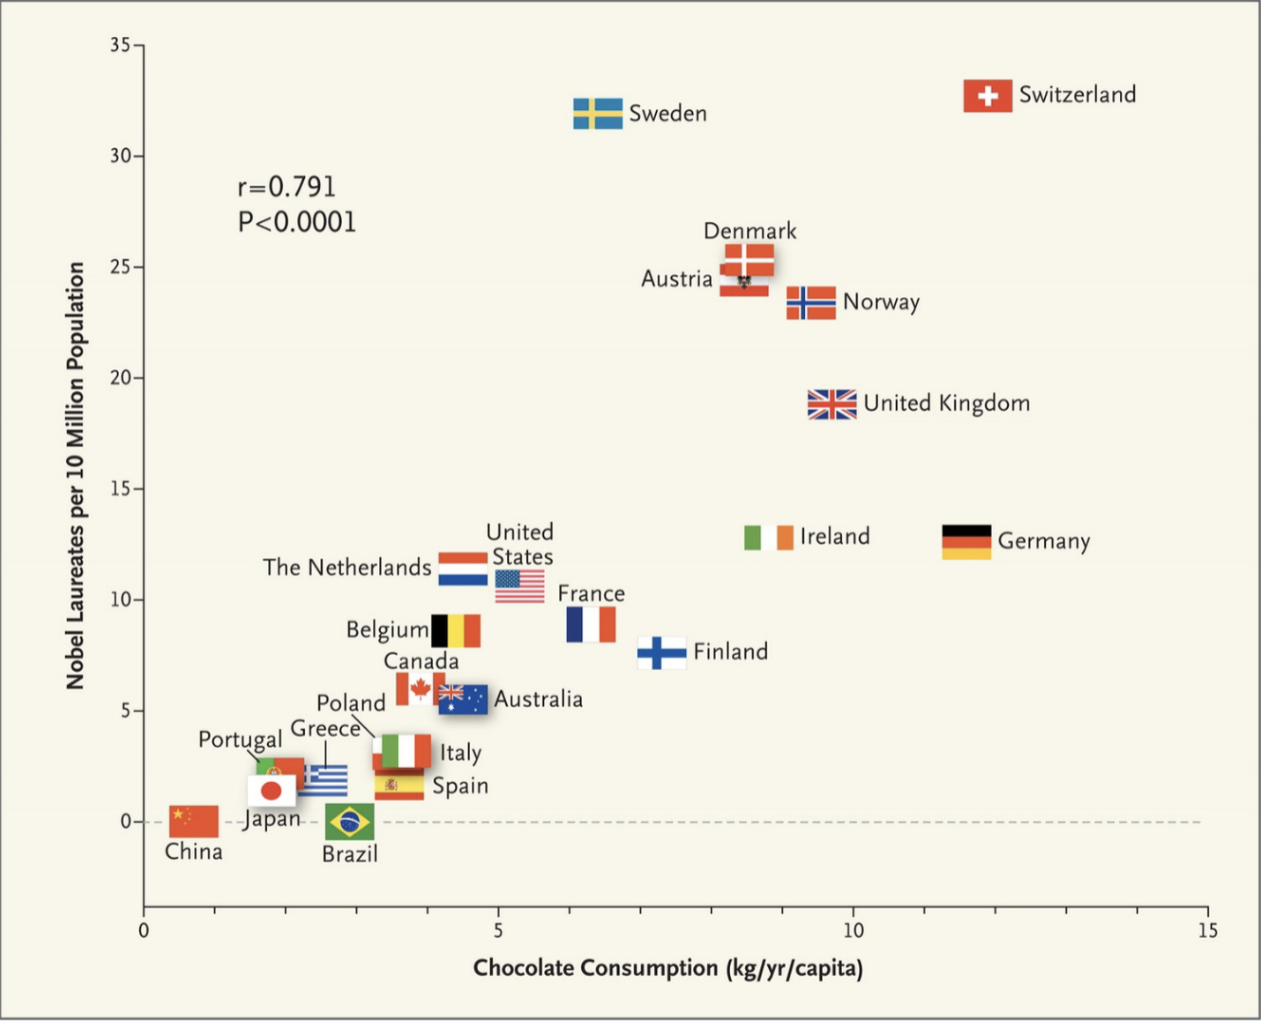
\includegraphics[width=0.75\linewidth]{images/01_chocolate} 

}

\caption{Chocolate Consumption and Nobel Prizes}\label{fig:chocolate}
\end{figure}

In Figure \ref{fig:chocolate}, the number of Nobel laureates per 10 million of the population (vertical axis) is plotted against the chocolate consumption in kilograms per capita in a given year (horizontal axis). As is clear in this graph, countries with higher rates of chocolate consumption also tend to have higher rates of Nobel laureates is an example of a \textbf{correlation}. A correlation is any statistical is any relationship between two variables.

Correlations can be very interesting. In many cases they can lead to new research questions. But they don't often answer the questions social scientists are actually interested in. We are generally interested in understanding \textbf{causal relationships} between variables.

To understand causal relationships, let's again consider the relationship between chocolate consumption and Nobel prizes. Do you think that if the U.S. wanted to increase the number of Nobel laureates, they should invest in chocolate and include chocolate in lunch meals for students? Probably not! It's unlikely that increased chocolate consumption \textbf{causes} an individual to win a Nobel prize. In this case, it is more likely that this correlation in the data just arose due to chance. Therefore, we have uncovered a \textbf{spurious correlation}, or a correlation that arose due to chance. There are many interesting spurious correlations. If you are interested in looking through some fun spurious correlations, just follow this \href{https://www.tylervigen.com/spurious-correlations}{link}. For example, you probably would not guess that consumption of mozzarella cheese is correlated with civil engineering doctorates awarded, but see Figure \ref{fig:spurious} for this surprising correlation.

\begin{figure}

{\centering 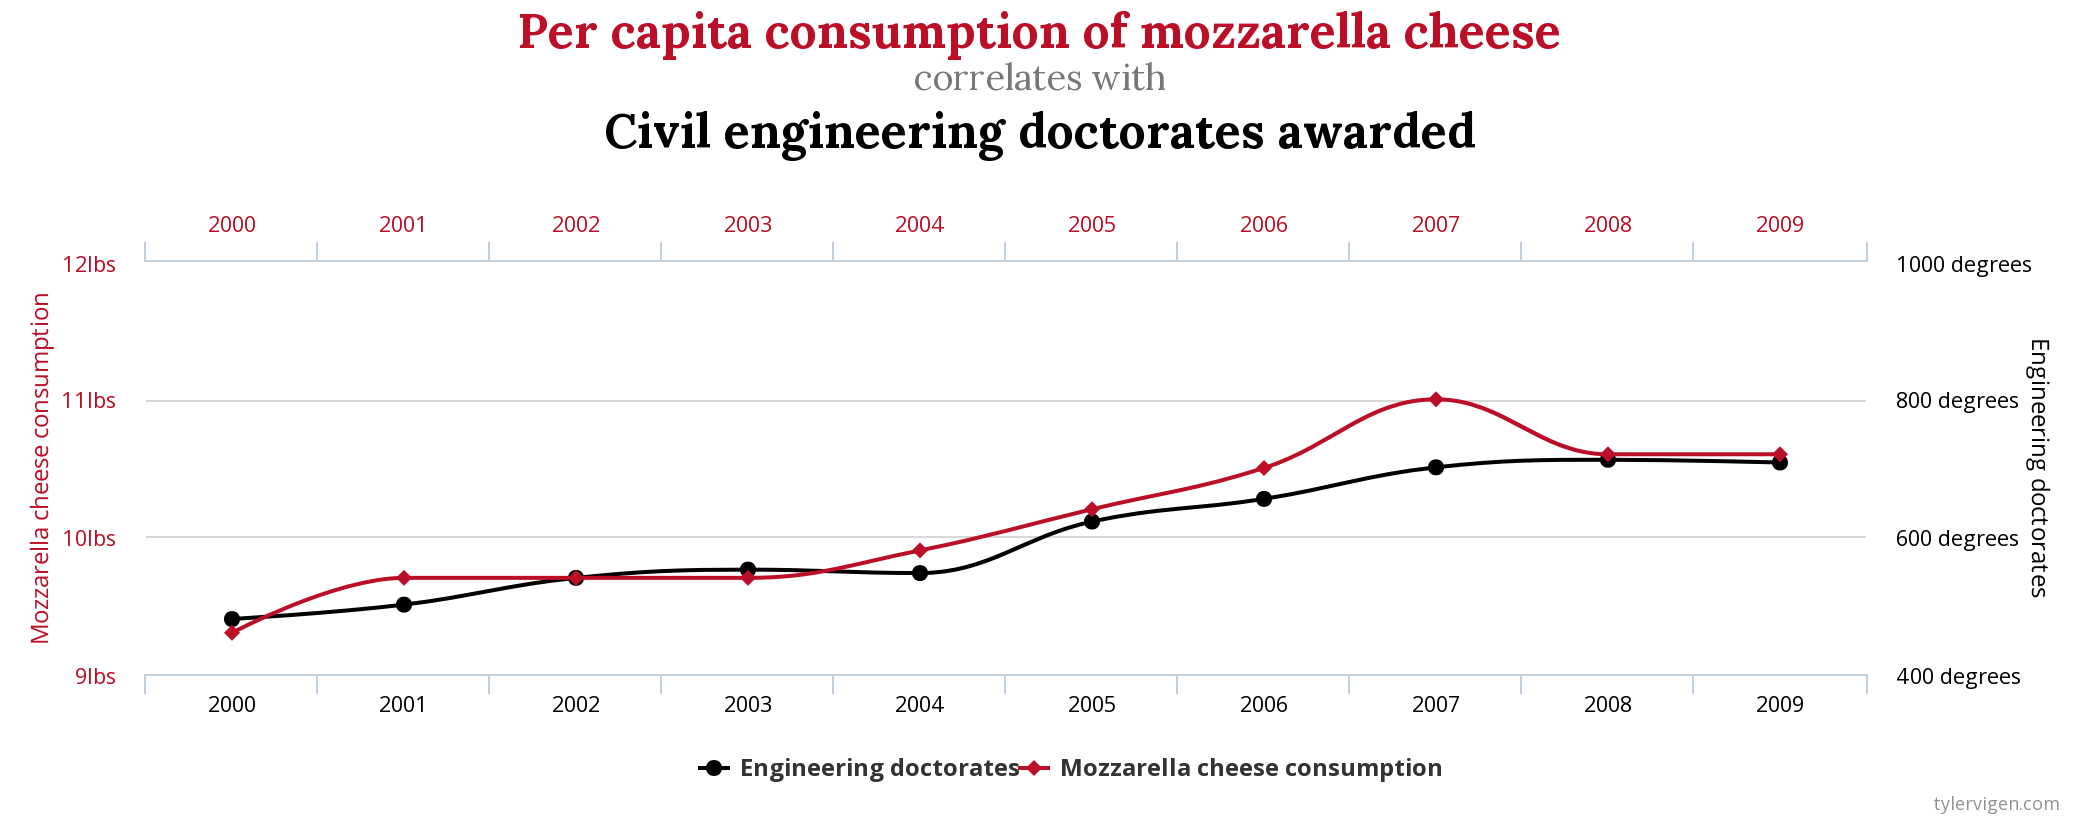
\includegraphics[width=1\linewidth]{images/01_spurious} 

}

\caption{Example of a Spurious Correlation from tylervigen.com}\label{fig:spurious}
\end{figure}

If we need to decide whether a given policy is worth it or not, we need to understand how it causally impacts individual's outcomes. To see why, let's imagine a high school is trying to decide whether to invest in a new after-school program designed to help students with SAT prep. Currently, they do not have such a program on campus, but they know some of their students attend programs offered outside the school. In order to try and understand the benefits of the program, the school decides to use data on past students to see if those who attended SAT prep programs outperformed students that did not.

The school finds those who attended SAT test prep programs score much higher on the SAT than those who did not. Does this mean the SAT test prep program works and the school should invest in one? Maybe, maybe not. There are two stories that could potentially rationalize this finding. Story 1 is that the programs are effective ways for students to learn the material they need to perform well on the SAT. That is, the program has a causal impact on SAT scores. Story 2 is that the programs are not actually effective. However, students that self-select into SAT programs also tend to be more motivated overall. They could, in theory, vary along many dimensions: academic ability, interest in college, parental background. It could be that any of these differences are actually driving the differences in SAT scores.

With only \textbf{observational data} it is difficult to tell which story is true. However, there is along-established way to identify causal relationship in medicine: the randomized control trial (RCT). To understand RCTs, imagine we are testing whether a given drug reduces blood pressure. To study the effectiveness we recruit a group of participants. Half of the participants are randomly placed into the \textbf{treatment} group and given the drug. The other half are placed into the \textbf{control} or \textbf{placebo} group and given a placebo drug. Now we can just compare outcomes for the two groups over time to understand the impact of the drug.

The key to a well-done experiment is \textbf{randomization}. If who receives the treatment is completely random, then on average, the two groups will be very similar. For example, in our test prep example, if we could randomly split students into two groups: test prep vs.~no test prep, then we could evaluate the impacts of the program. Since students are no longer self-selecting into the program, there should be little difference in the two groups in terms of academic ability, college interest, parental background.

Not all questions in social science can be answered with an experiment. In certain cases it may be prohibitively expensive or unethical to run an experiment. However, if an experiment can be done, it is hard to find more convincing evidence. Experiments have been widely influential in many social sciences. For example, in the field of development economics, a large number of experiments have been undertaken in order to develop policies aimed at alleviating global povery. In 2019, Abhijit Banerjee, Esther Duflo, and Michael Kremer won the Nobel Prize in Economics ``for their experimental approach to alleviating global poverty.''

In this course, we will be studying a number of social science experiments. Our first experiment comes from Brownback and Sadoff (2020). The motivation for this experiment is a startling statistic. Only 40 percent of community college students earn a college degree within 6 years (Shapiro et al.~2017). Given these poor outcomes, it is important to consider tools to improve performance. In Brownback and Sadoff (2020) the researchers explore one potential tool that has been previously unexplored: financial incentives to instructors. This is often referred to as a pay-for-performance model. Instructors are paid for how well their students perform. While prior experiments have studied this model in some settings, no prior work has explored how this would function in the community college setting.

Brownback and Sadoff (2020) run the following experiment at a community college in Indiana (Ivy Tech):

\begin{itemize}
\tightlist
\item
  Some instructors (the treatment group) received \$50 for each student that passes an externally-administered test
\item
  Other instructors (the control group) did not receive such an incentive.
\end{itemize}

The key in their design is that the instructors that are chosen to receive the incentives are randomly selected. Therefore, they are not, on average, better teachers than instructors in the control group. Therefore, if we observe any difference in student performance between the treatment and control, then it must be due to the financial incentives for instructors.

\textbf{Summary}: Social scientists are often interested in causal relationships. One way to study causal relationships is through an experiment. The key aspect in an experiment that allows us to study causal relationships is that \textbf{treatment is randomized}.

\hypertarget{data-from-brownback-and-sadoff-2020}{%
\section{Data from Brownback and Sadoff (2020)}\label{data-from-brownback-and-sadoff-2020}}

In many disciplines, there has been a push toward transparency and replication. Past work has shown that some very influential studies have failed to replicate (See \href{https://en.wikipedia.org/wiki/Replication_crisis\#In_economics}{replication crisis}). A common way to provide transparency is to have authors make the data from their research publicly available. That means we will get to use the actual data from the experiments we are studying in this class.

Table \ref{fig:bsdata} shows a selection of the data from Brownstone and Sadoff (2020). The actual data is much larger, but only a subset of the variables will be relevant for our analysis. This is referred to as a \textbf{data table}. Each \textbf{row} in a data table is an \underline{observation}, while each \textbf{column} is a variable.

\begin{figure}

{\centering 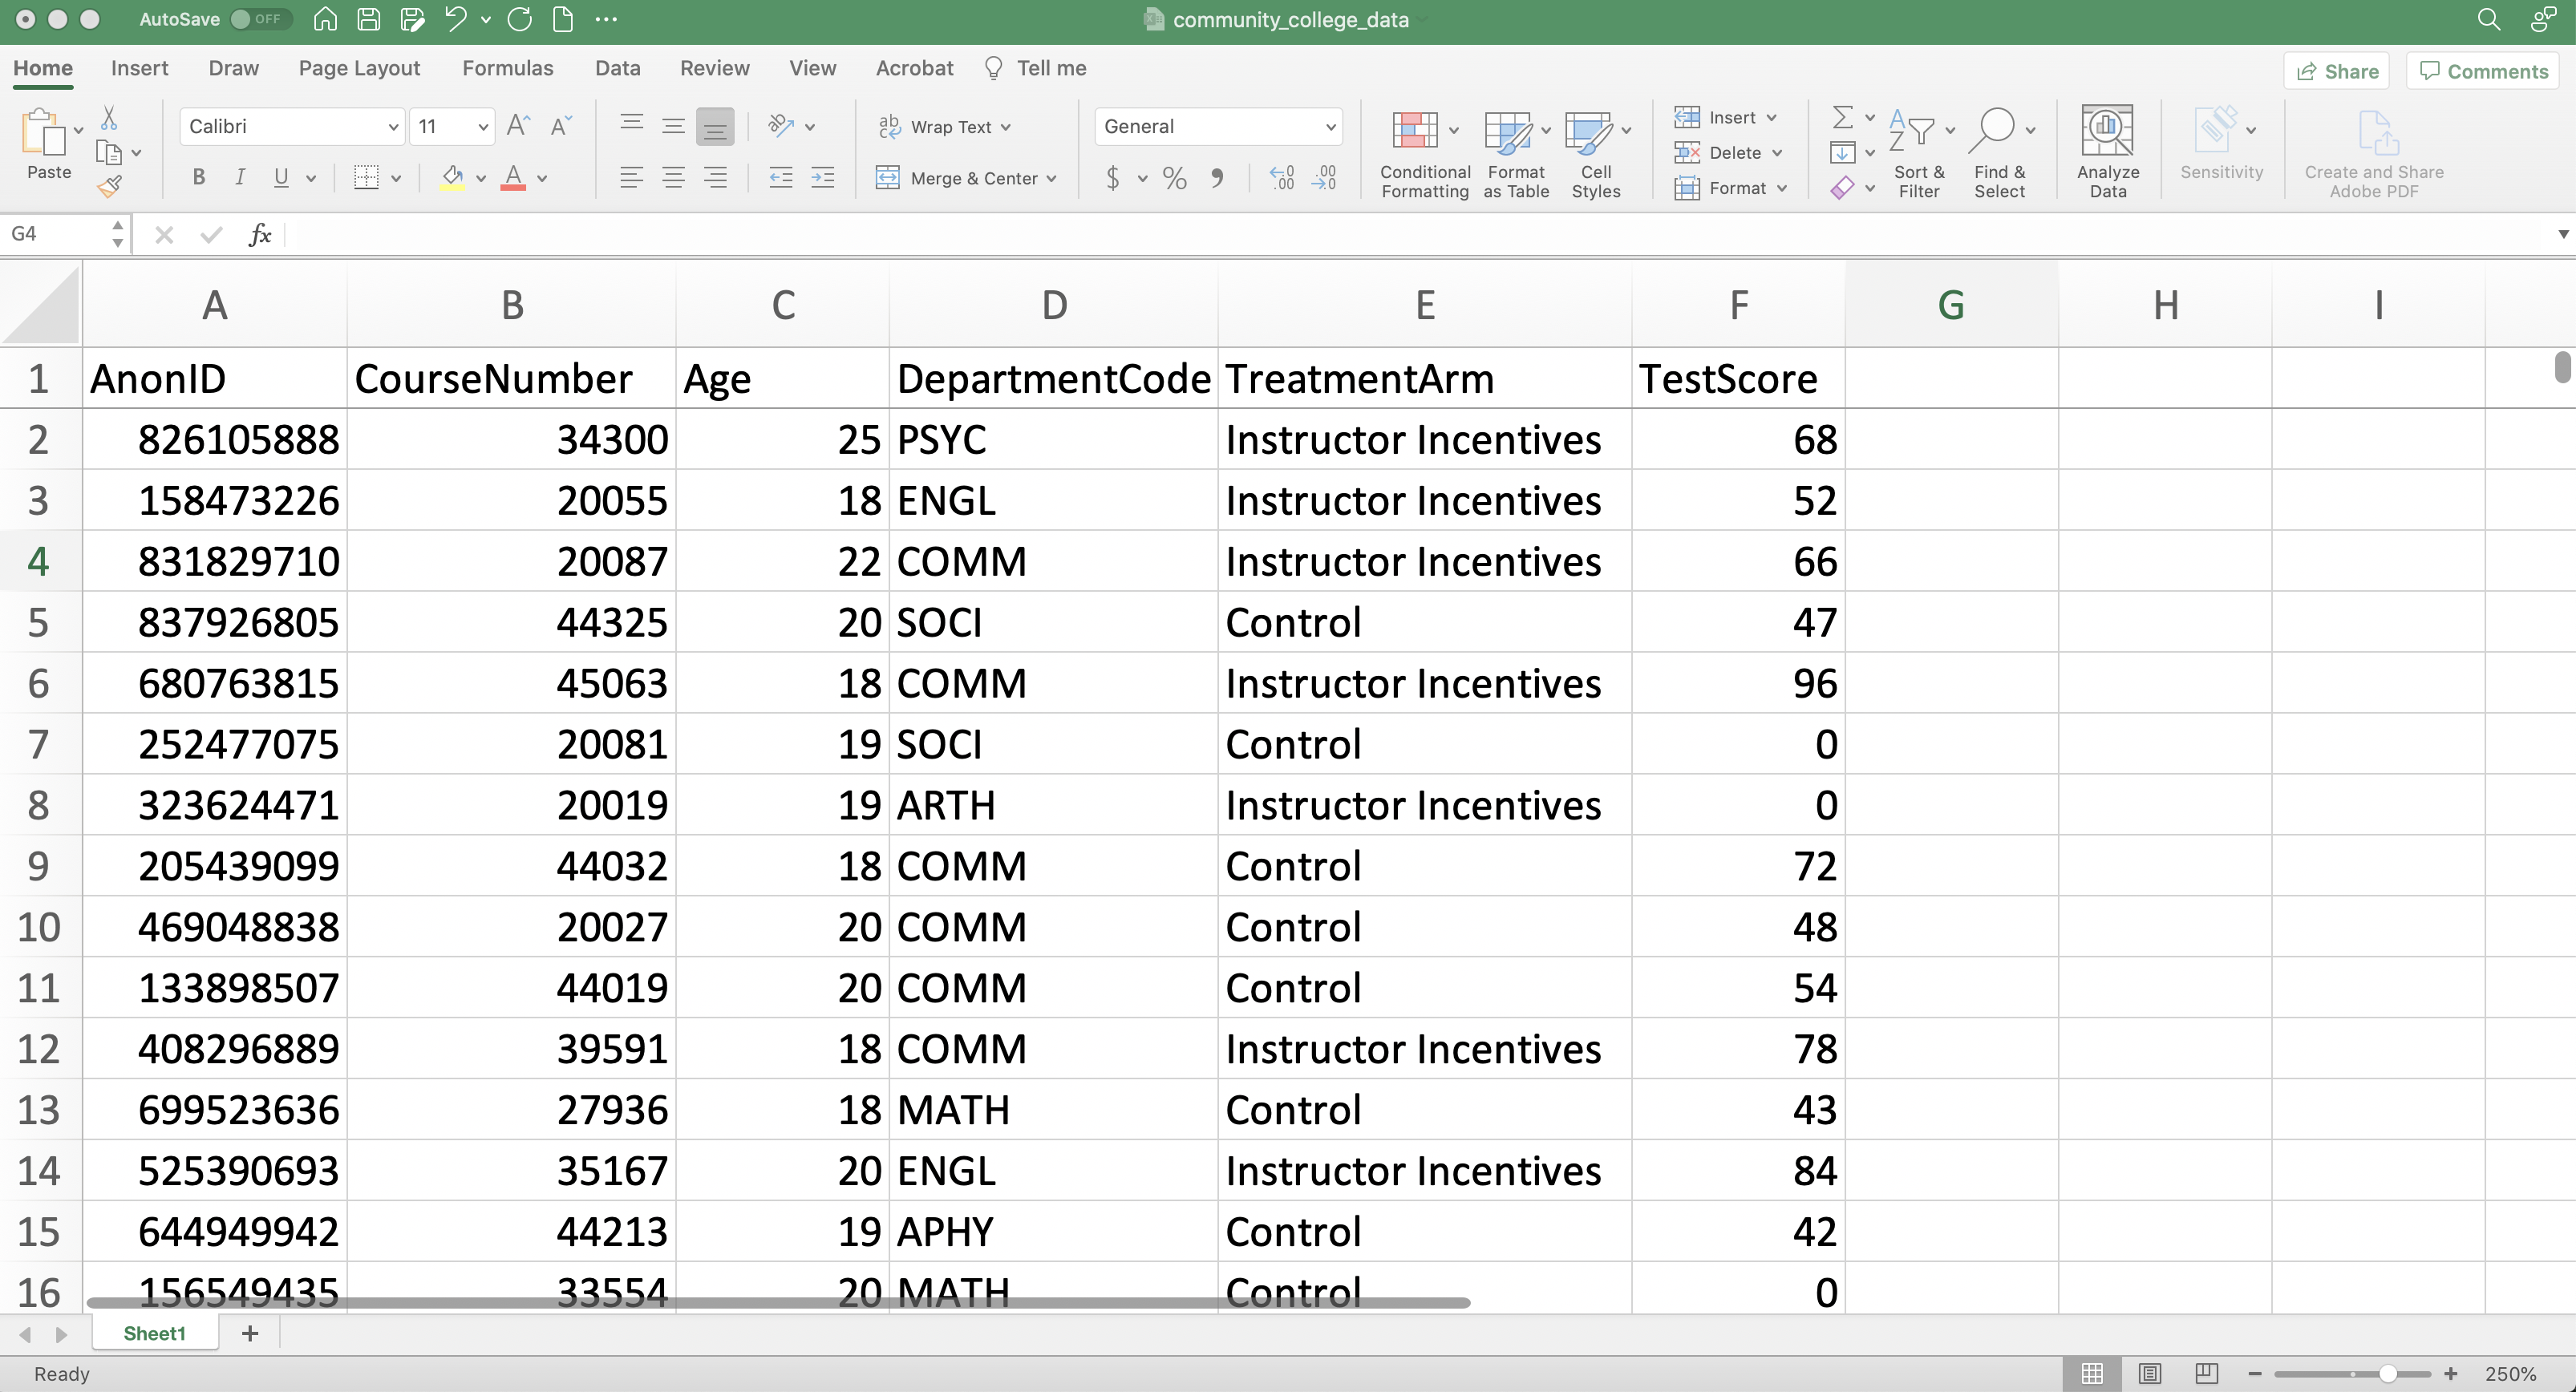
\includegraphics[width=0.75\linewidth]{images/01_data} 

}

\caption{Data From Brownstone and Sadoff (2020)}\label{fig:bsdata}
\end{figure}

It is always important to understand the structure of your data before proceeding with any data analysis. One of the most important components of understanding the structure is to discern the \textbf{unit of observation}. The unit of observation is the level at which the data is reported. To discern it for yourself, just think about what each row of the dataset represent. Is each row an individual, a neighborhood, a country, a state? To practice, let's go through a few examples.

What is the unit of observation in Table \ref{fig:student}?

\begin{figure}

{\centering 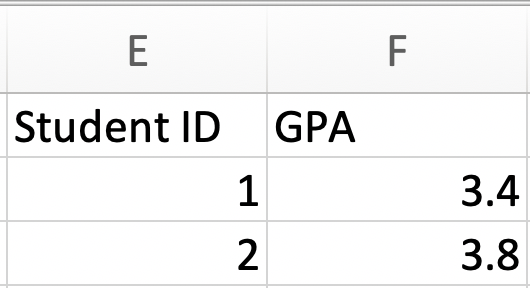
\includegraphics[width=0.5\linewidth]{images/01_student} 

}

\caption{Unit of Observation Example 1}\label{fig:student}
\end{figure}

To answer this question, we need to decide what a row represents. In this case, each row corresponds to a different student. Therefore the observation level is a student.

What is the unit of observation in Table \ref{fig:studentterm}?

\begin{figure}

{\centering 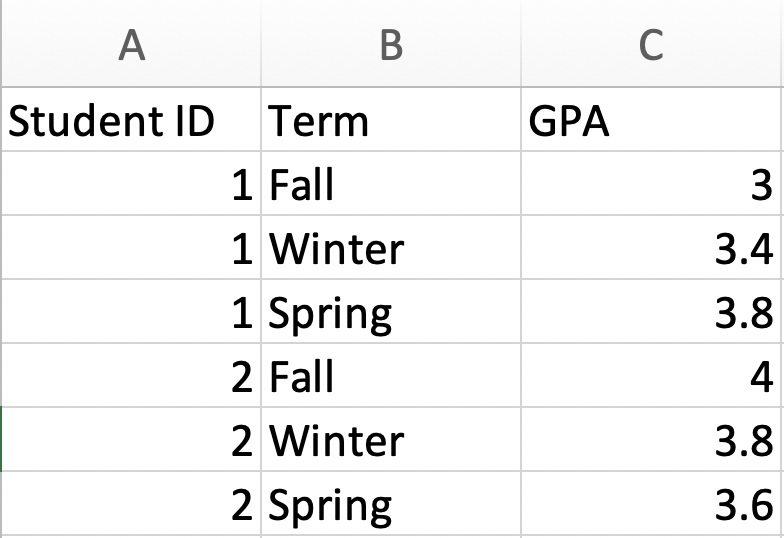
\includegraphics[width=0.55\linewidth]{images/01_student_term} 

}

\caption{Unit of Observation Example 2}\label{fig:studentterm}
\end{figure}

Again, we need to decide what a row represents. In this case, each row corresponds to a different student in a different term. Therefore the observation level is a student-term.

Now let's think about what the unit of observation is in the Brownstone and Sadoff (2020) data. The variable \textbf{AnonID} is the identifier for a student. The variable \textbf{CourseNumber} is the identifier for a course. This dataset seems to be giving us the information for a student in a given course. Therefore the observation level is a student-course.

Before we get to analyzing the data, let's actually learn about our first feature in Excel. When browsing an excel file, it is often convenient to \textbf{freeze} the first row so that it is always visible. In our case, the first row holds variable names. Therefore, if we freeze the first row we can scroll through the data without having to remember what each column corresponds to.

To freeze the first row go to the \textbf{View} and then click \textbf{Freeze Top Row} (See \ref{fig:freeze}).

\begin{figure}

{\centering 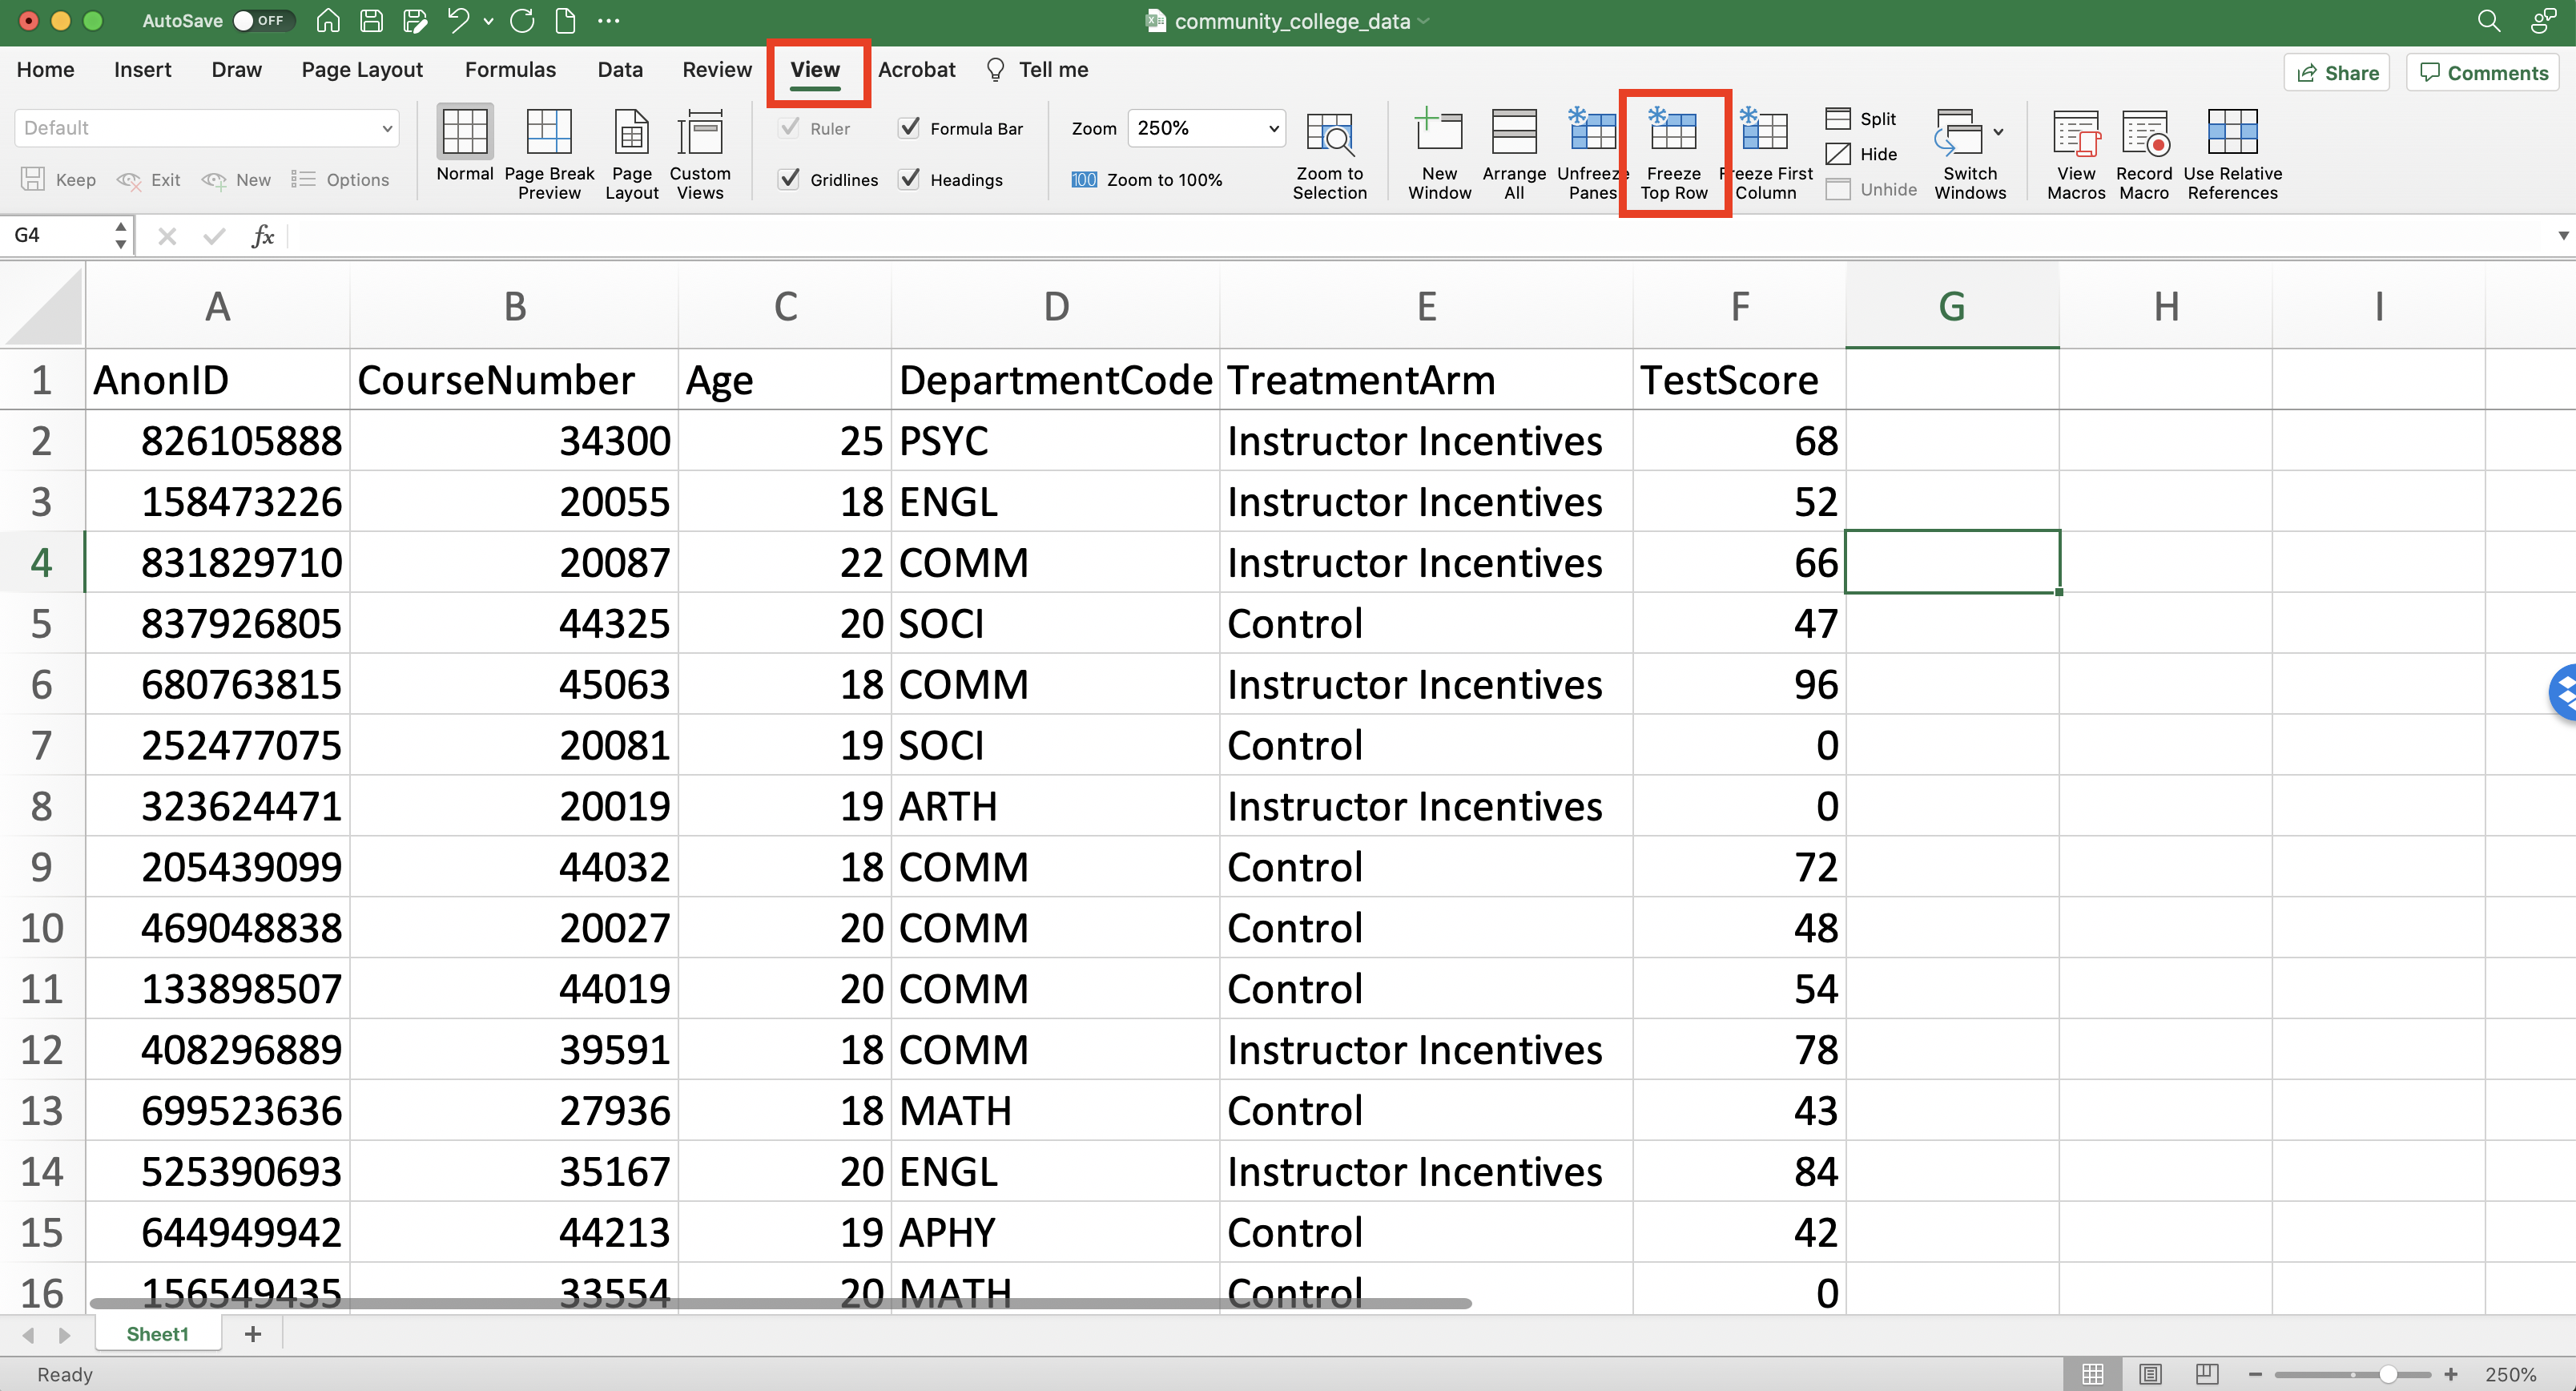
\includegraphics[width=1\linewidth]{images/01_freeze} 

}

\caption{Freezing the First Row}\label{fig:freeze}
\end{figure}

Let's talk a little bit about our goal with this dataset. Our goal is to determine if providing financial incentives to teachers impacts student performance. The variable \textbf{Treatment Arm} details whether a student has an instructor that received incentives or is in the control group. Therefore, we can see if test scores improve based on the Treatment Arm of the student. To perform this analysis, we need to learn how to use \textbf{functions} in Excel.

\hypertarget{statistical-functions}{%
\section{Statistical Functions}\label{statistical-functions}}

A function is something that takes in an input and produces an output. For example, you can think of taking the average as a function. The input is a list of numbers, and the output is the average of that list of numbers. When the inputs and outputs of a function are numbers (as it is in this example), then it is a \textbf{statistical function}.

In Excel, statistical functions are extremely important to understand. If you are doing research, it is common to start out with a list of summary statistics. If you are in business, it might be important to know some summary statistics about your products, sales, costs, etc. To create summary statistics these summary statistics, we use statistical functions.

In order to illustrate the use of statistical functions, let's consider the following dataset that has information on Gross Domestic Product (GDP) for ten countries

\begin{figure}

{\centering 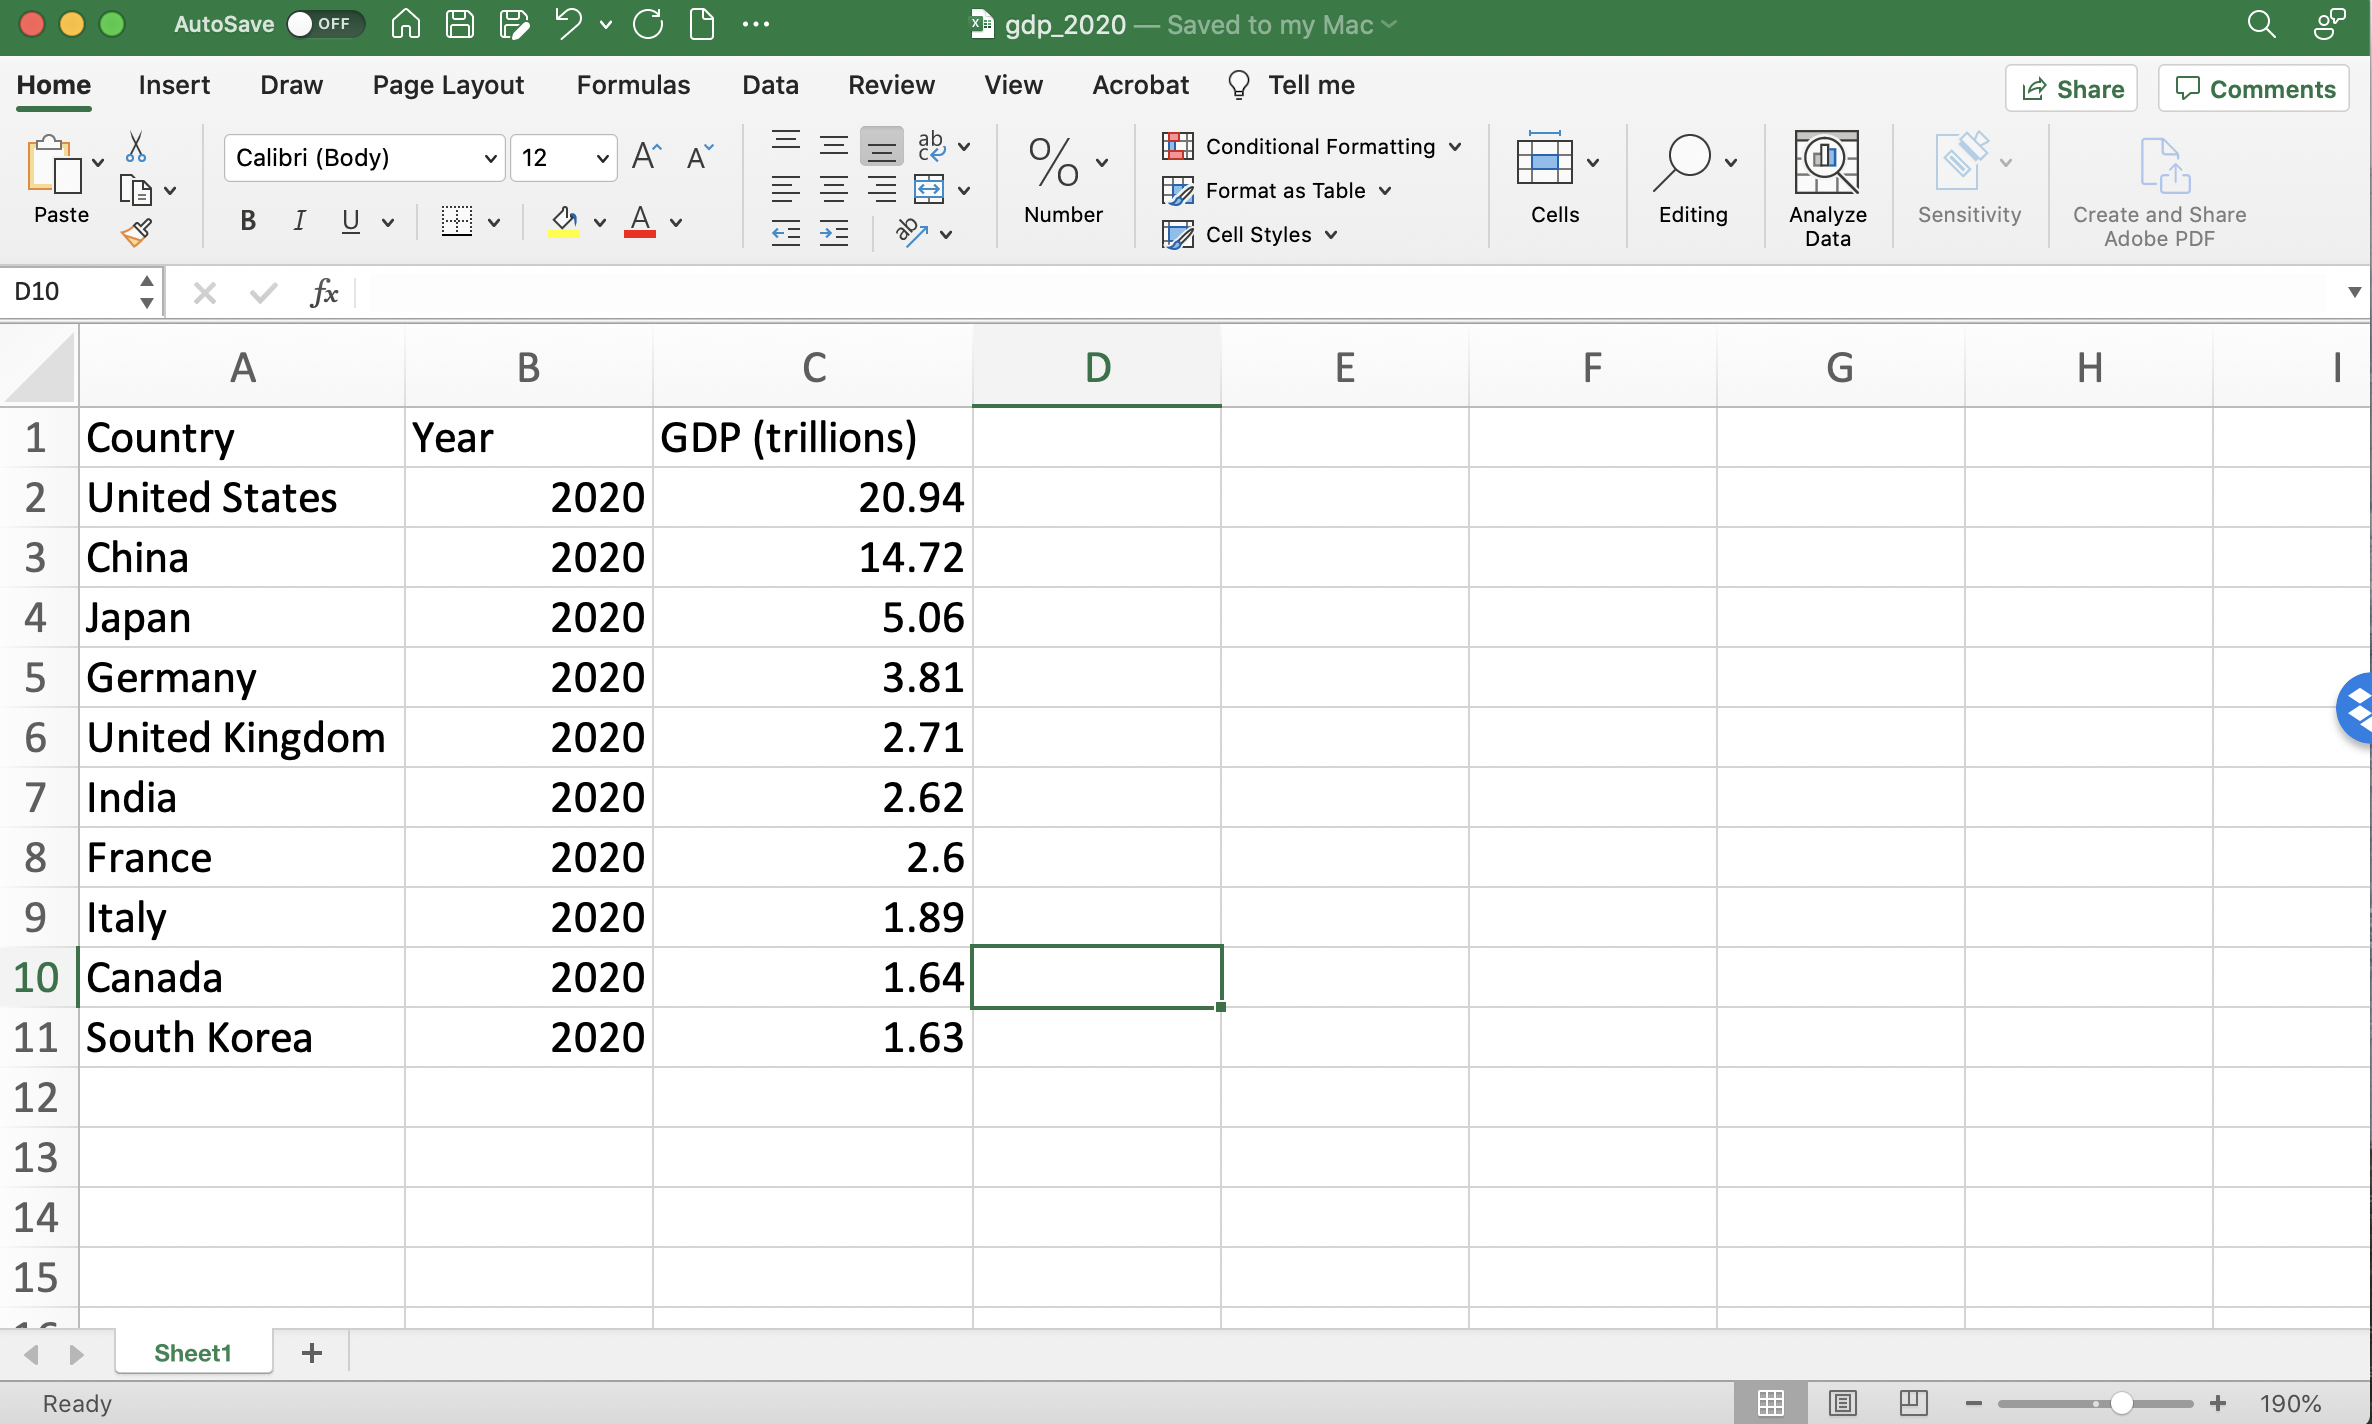
\includegraphics[width=1\linewidth]{images/01_gdp2020} 

}

\caption{GDP in 2020}\label{fig:gdp2020}
\end{figure}

Let's introduce our first statistical function: the \texttt{AVERAGE} function. This function will take in a list of numbers and output the average of all those numbers. There are many statistical functions in Excel, including:

\begin{itemize}
\item
  \texttt{COUNT} -- counts the number of numbers
\item
  \texttt{SUM} -- adds up the numbers
\item
  \texttt{AVERAGE} -- averages the numbers
\item
  \texttt{MEDIAN} -- retrieves the median of all numbers
\item
  \texttt{MAX}, \texttt{MIN} -- retrieves the maximum and minimum of all numbers
  respectively
\item
  \texttt{MODE} -- retrieves the mode of all numbers
\end{itemize}

In order to make use of statistical functions, we first need to learn how to reference cells. In Excel, every cell is identified by a column letter and a row number. For example, in \ref{fig:japan} I have clicked on the cell that holds the word ``Japan''. This entry is in column A of row 4. Therefore, this is cell A4.

\begin{figure}

{\centering 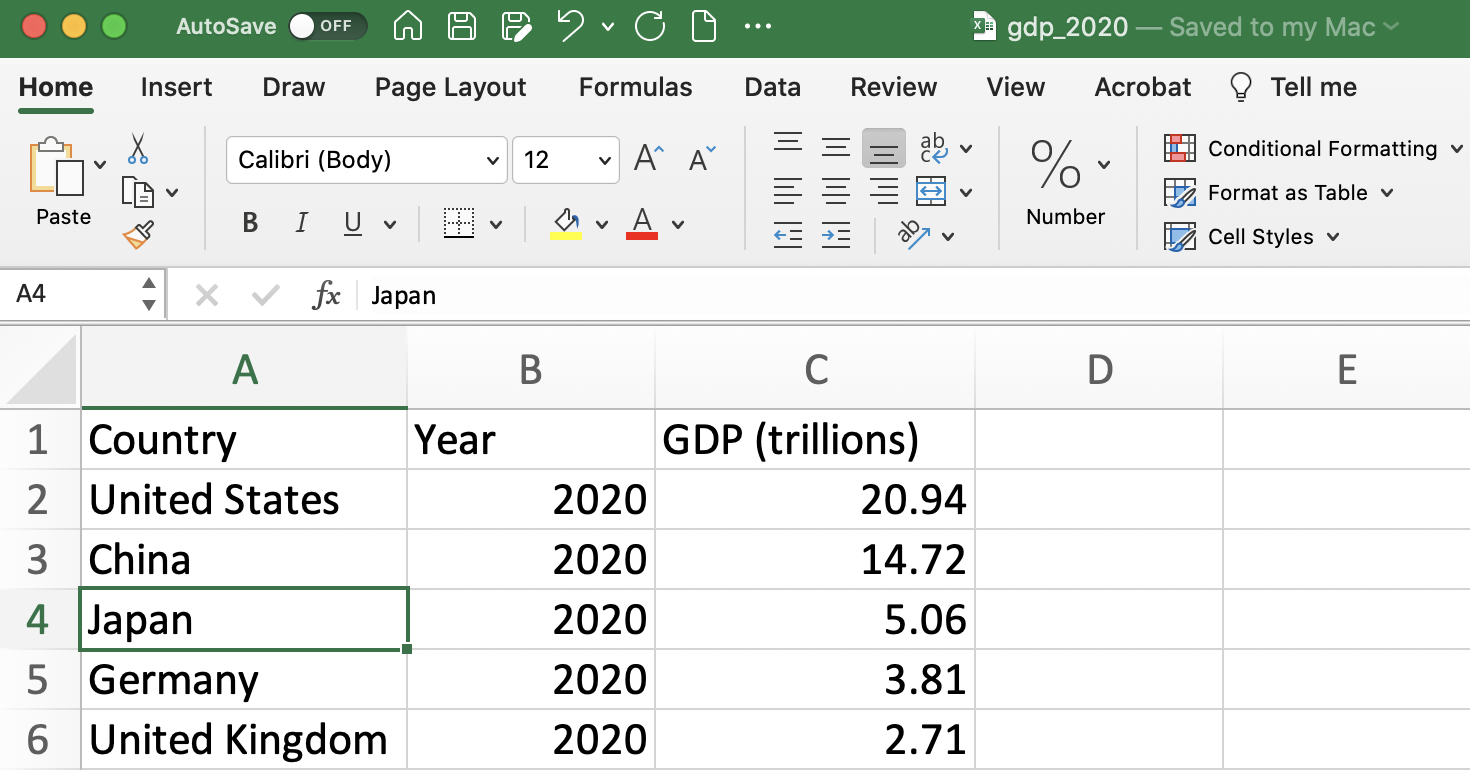
\includegraphics[width=1\linewidth]{images/01_japan} 

}

\caption{How to Reference a Cell}\label{fig:japan}
\end{figure}

You can also reference a range of cells (this will be useful when taking averages). For example, to reference rows 2-6 of column C we could type \texttt{C2:C6} (See \ref{fig:cells}). Whenever you read a colon in Excel, you should read it as ``through''. Therefore, the text \texttt{C2:C6} can be read as ``cells C2 through C6''.

\begin{figure}

{\centering 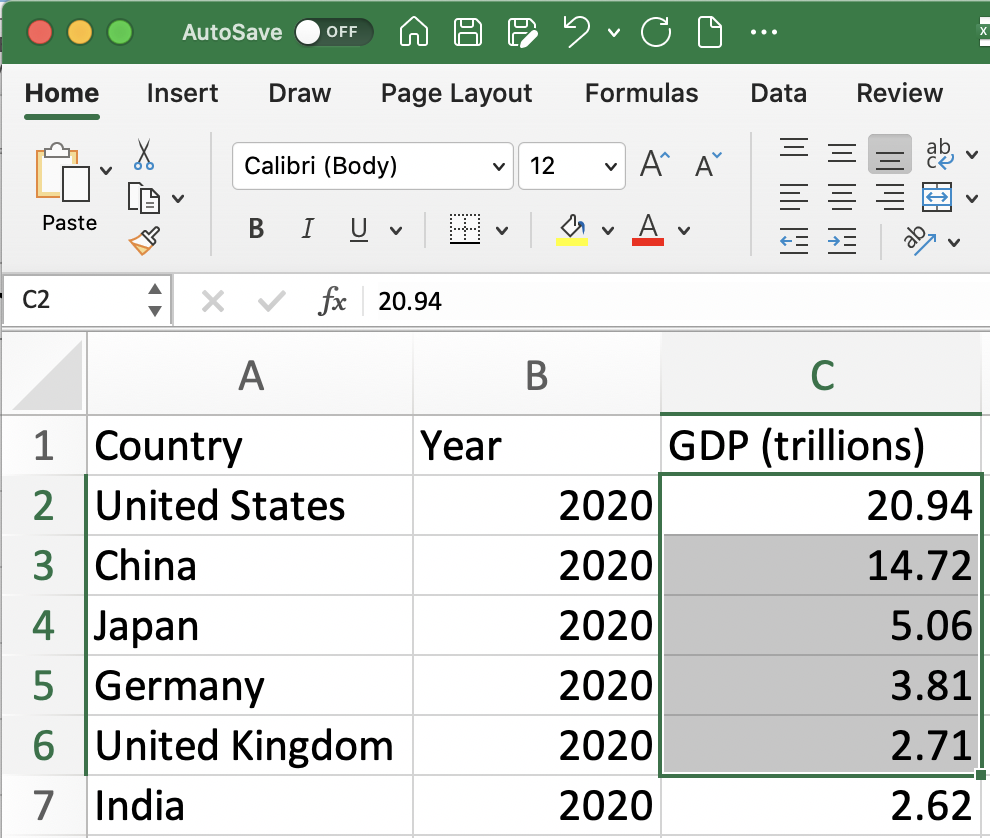
\includegraphics[width=0.7\linewidth]{images/01_cells} 

}

\caption{Referencing a Range of Cells}\label{fig:cells}
\end{figure}

Sometimes, it is helpful to reference an entire column. For example, later we will open an Excel spreadsheet that has thousands of students. In some cases, it will be helpful to reference an entire column when using statistical functions. For example, if we are interested in the average of a variable in column C, we can type \texttt{C:C} to reference the entire column.

Now that we understand how to reference cells, we can begin to apply functions. We will begin with the \texttt{AVERAGE} functions which can compute an average of a list of numbers. In our spreadsheet, we are interested in computing the average GDP across these ten countries. To do so, we can first click in an unpopulated cell and type:

\begin{center}
\colorbox{gray!20}{\texttt{=AVERAGE(C:C)}}
\end{center}

Note the \texttt{=} sign in the text above. This tells Excel to evaluate the function. If you omit the \texttt{=} you will find that the cell is just populated with the text \texttt{AVERAGE(C:C)} and not the average value of column C.

Figure \ref{fig:average1} depicts an example where we have set up a Summary Statistics table for this dataset. In cell F3, we have written the function that calculates the average GDP across these ten countries.

\begin{figure}

{\centering 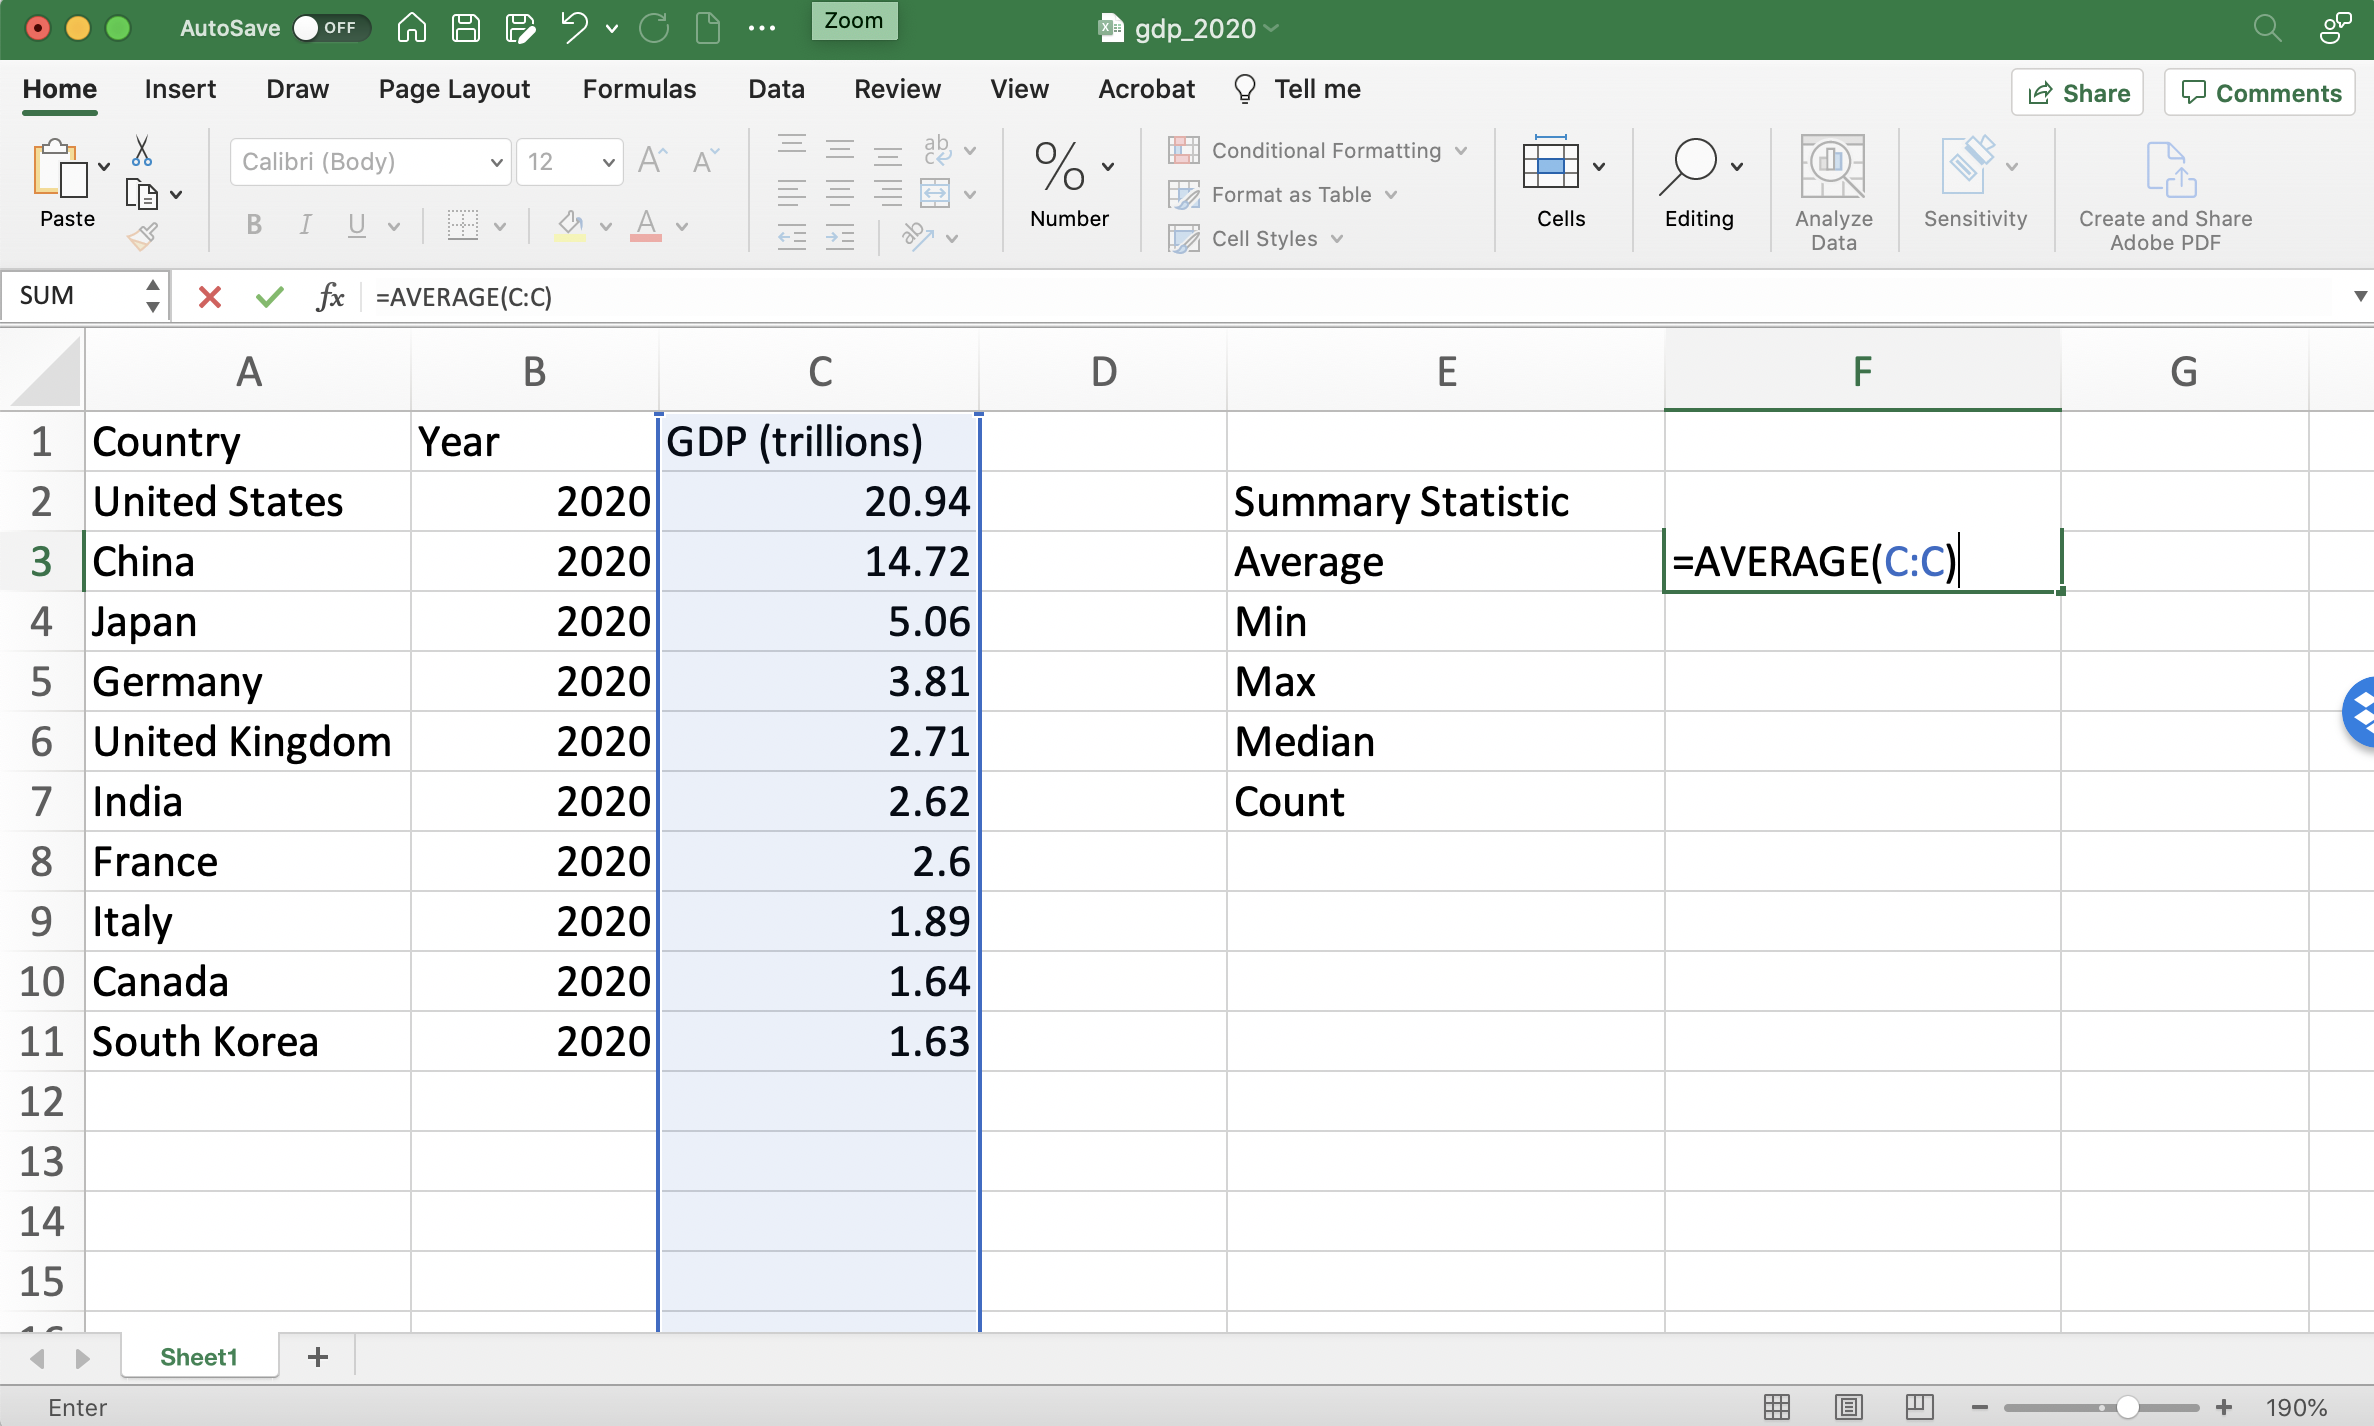
\includegraphics[width=0.8\linewidth]{images/01_average1} 

}

\caption{Computing Average GDP in 2020 (Before Pressing Enter)}\label{fig:average1}
\end{figure}

As soon as we present enter, the function will be evaluated and the average will appear in cell F3 (see Figure \ref{fig:average2}).

\begin{figure}

{\centering 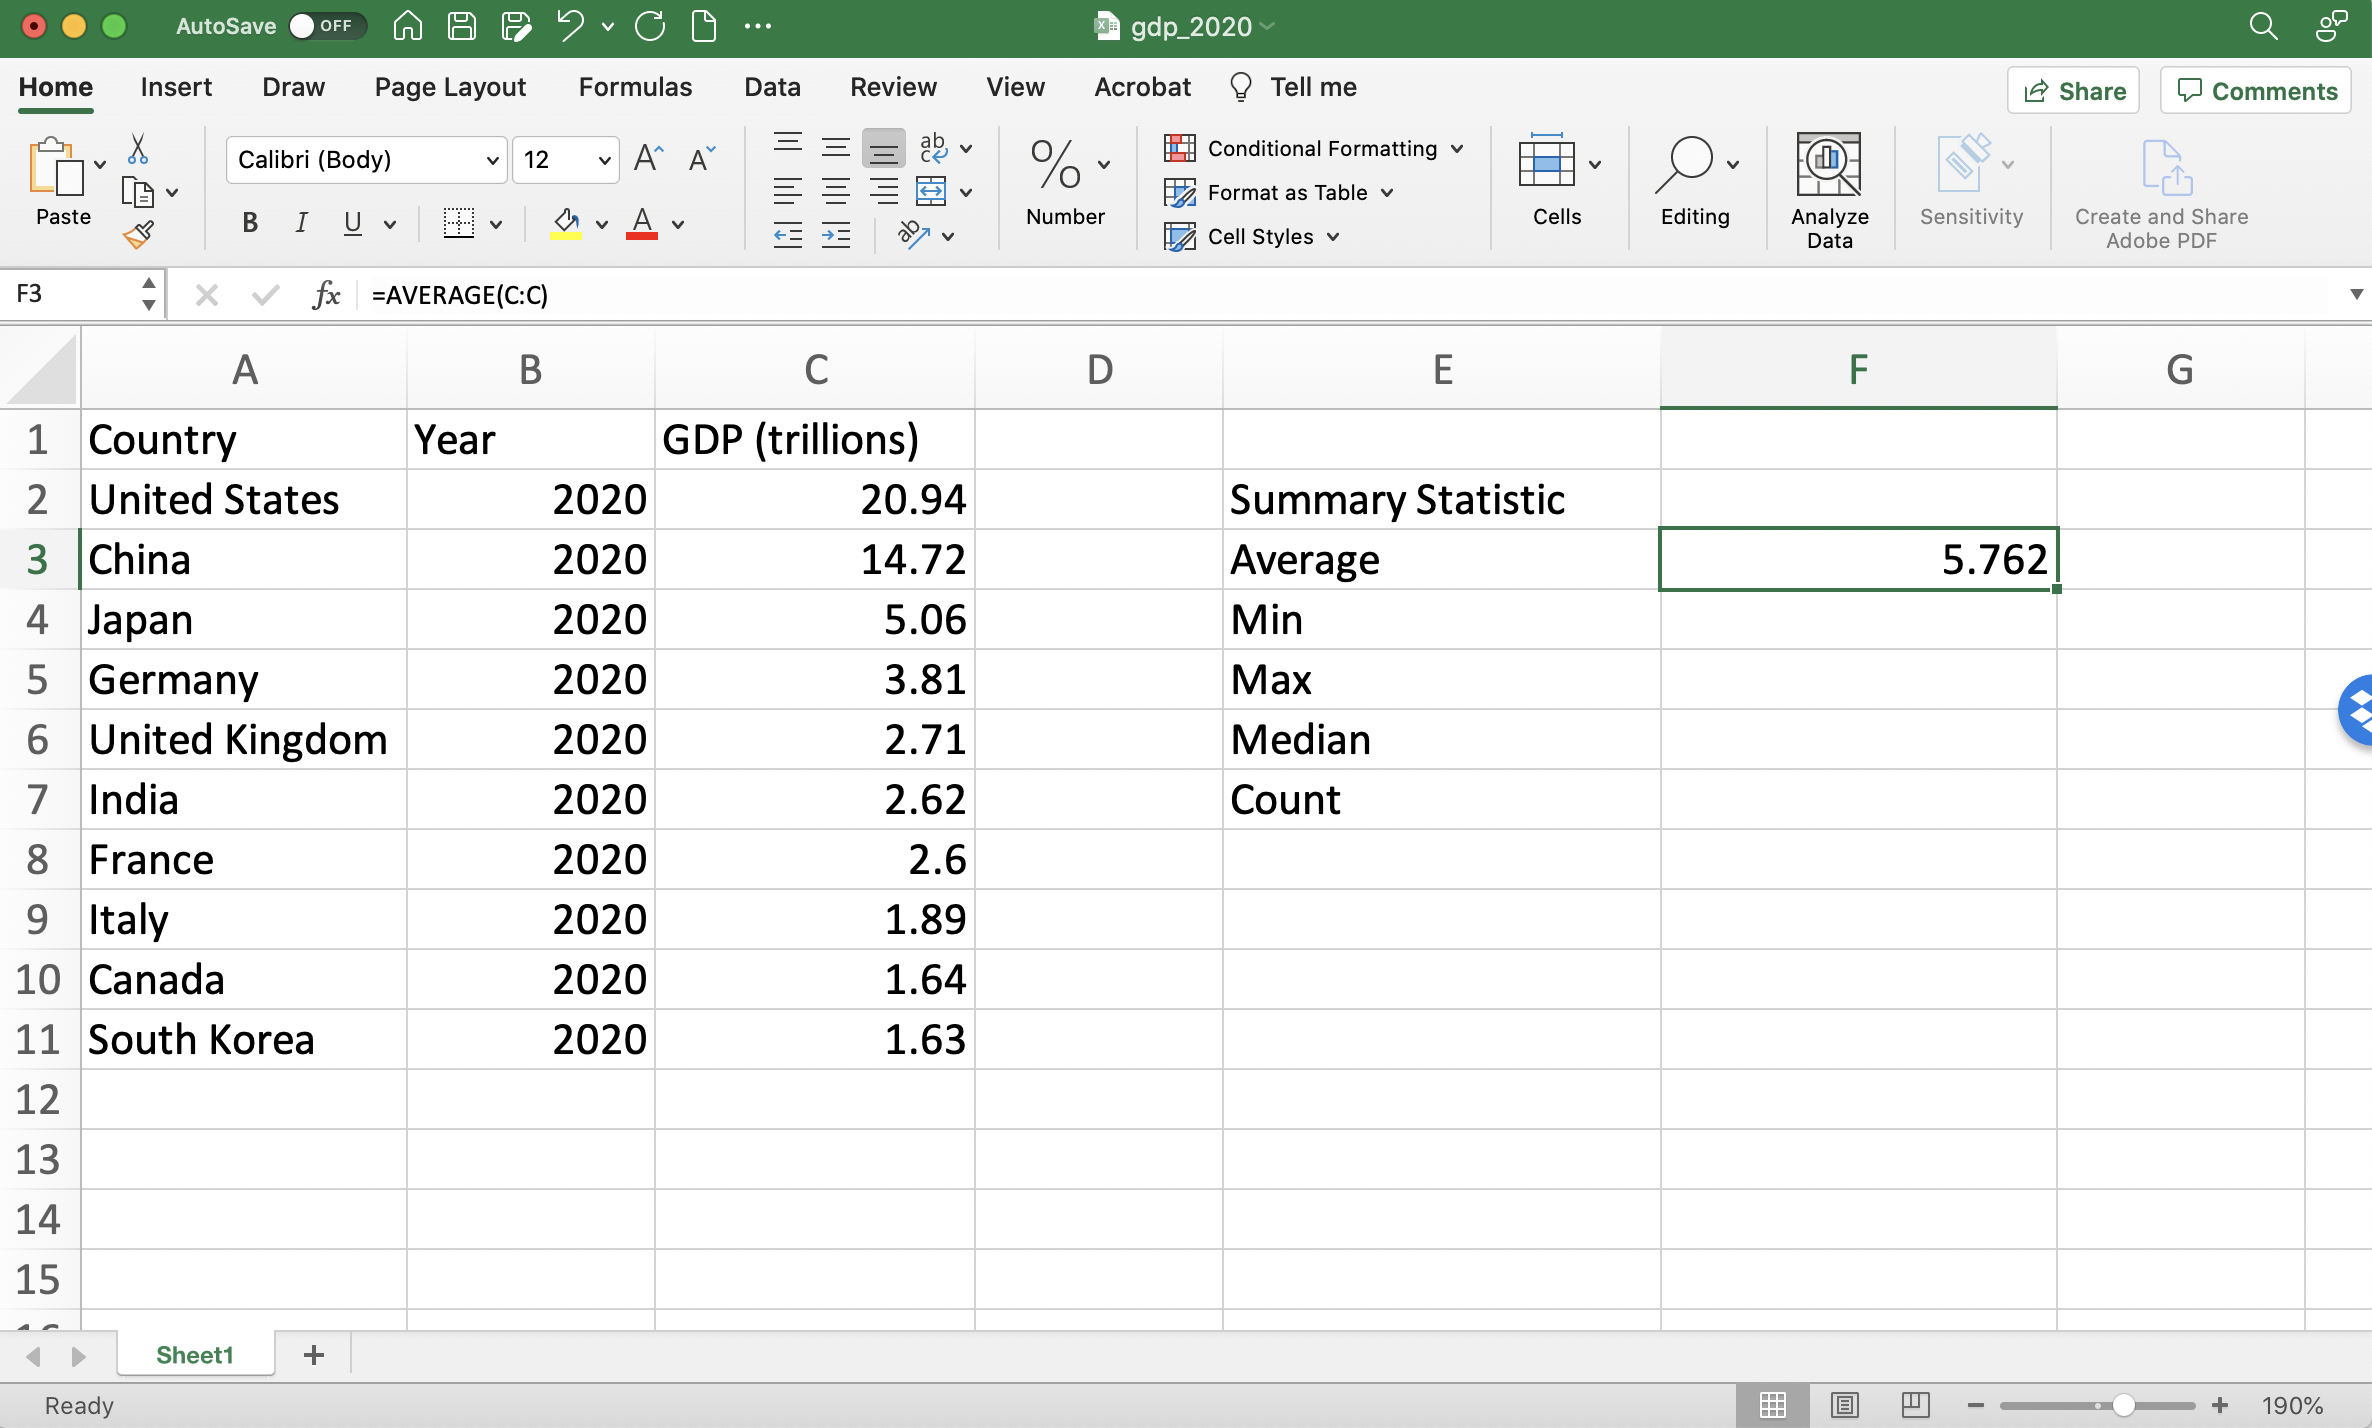
\includegraphics[width=0.8\linewidth]{images/01_average2} 

}

\caption{Computing Average GDP in 2020 (After Pressing Enter)}\label{fig:average2}
\end{figure}

The rest of the summary statistics are completely analogous, replacing \texttt{AVERAGE} with the relevant function. See Figure \ref{fig:gdpsumstats} for the output of the rest of the Summary Statistics table.

\begin{figure}

{\centering 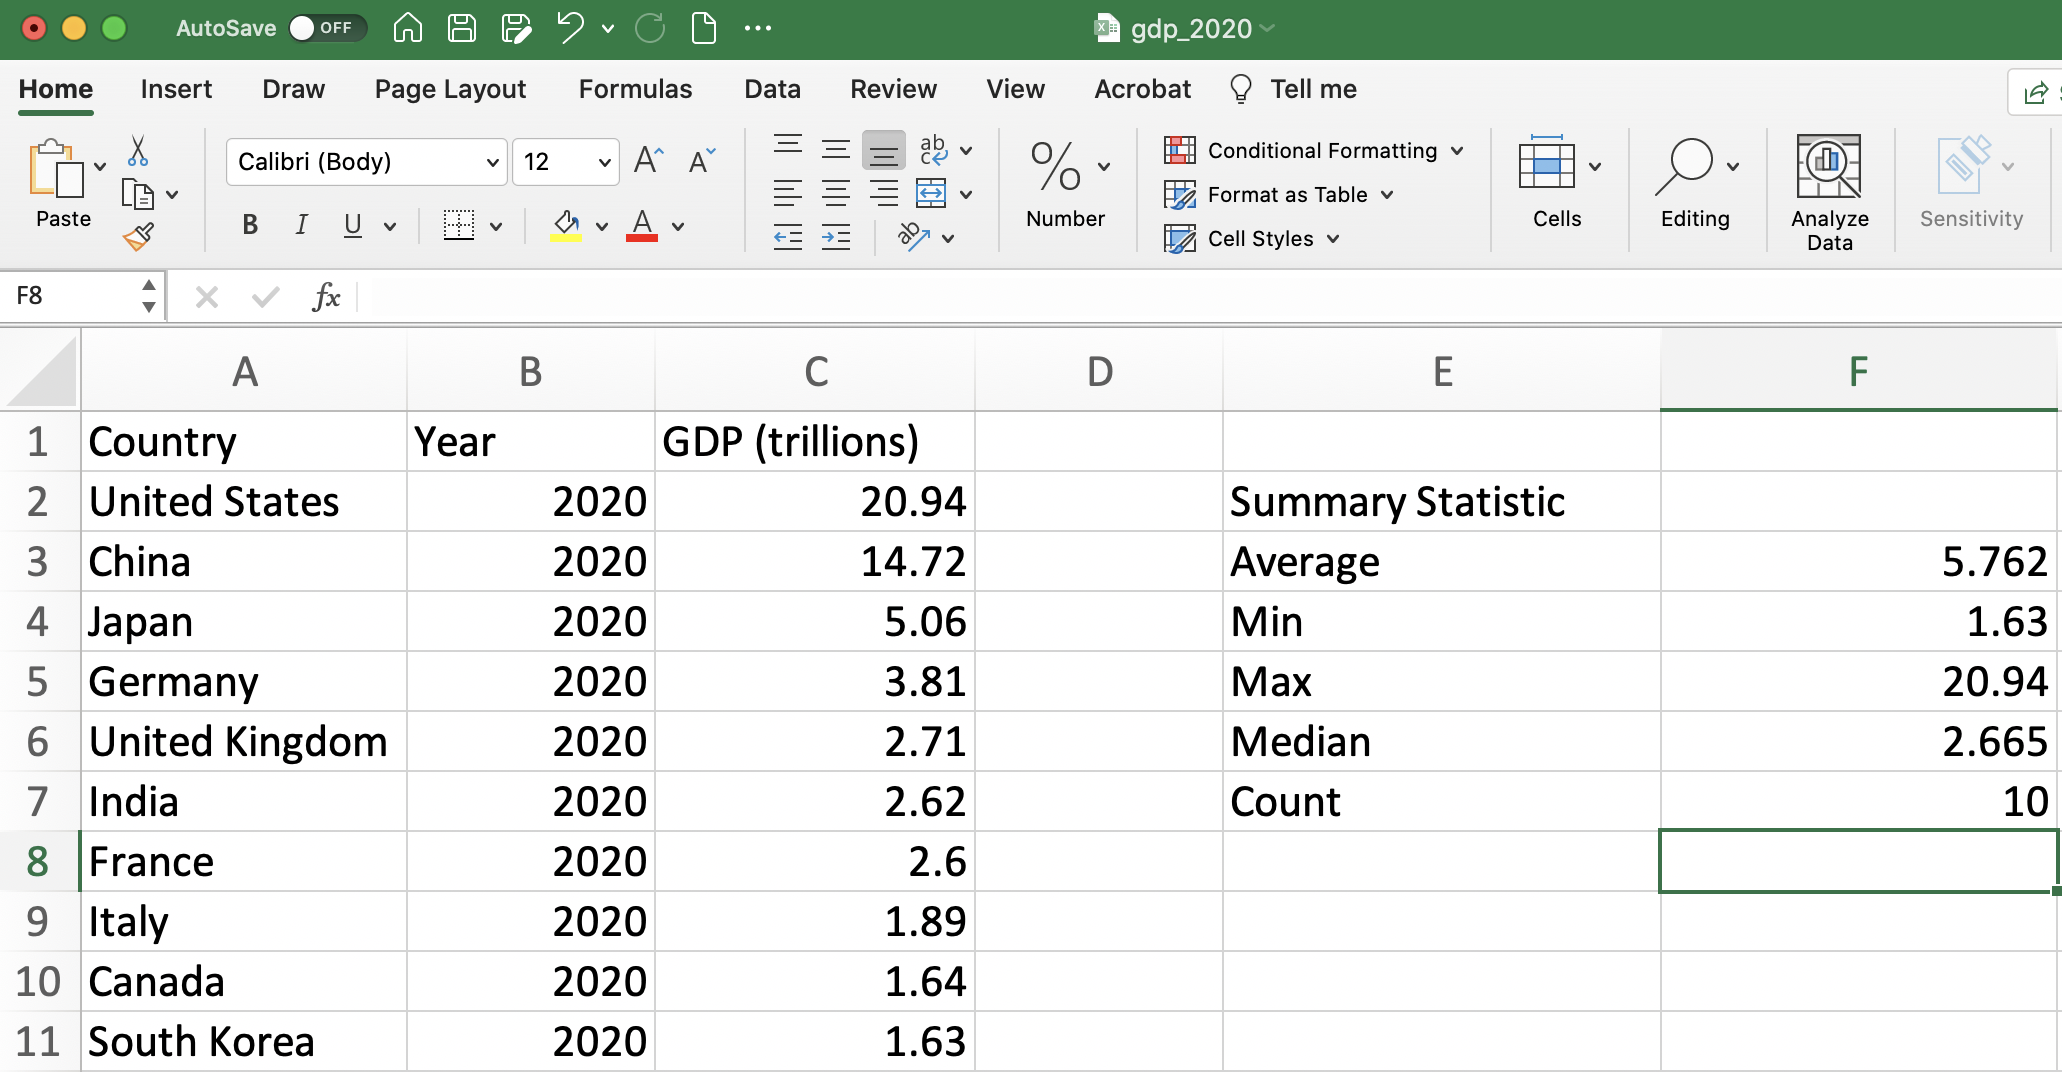
\includegraphics[width=0.8\linewidth]{images/01_gdp_sum_stats} 

}

\caption{Summary Statistics Table}\label{fig:gdpsumstats}
\end{figure}

\hypertarget{logical-functions}{%
\section{Logical Functions}\label{logical-functions}}

Another type of function in Excel is called a \textbf{logical function}. Before learning about \textbf{logical functions} we need to learn more about logical statements in general. A logical statement is a statement that is either true or false. For example, all of the following statements are either true or false.

\begin{itemize}
\item
  ``The student passed the class''
\item
  ``The participant is in the treatment group''
\item
  ``The temperature is below freezing''
\end{itemize}

These statements are all either true or false. This type of binary logic is incredibly important in certain areas of mathematics as well as the development of computers. An entire branch of mathematics, termed \textbf{Boolean algebra}, deals with variables that take on binary values.

In Excel, we can type logical statements and Excel will evaluate whether the statement is True or False. The key is you need to type the statement in the correct format so that Excel understands what you are trying to ask.

For example, in our dataset on GDP in 2020, one example of a logical statement is: ``GDP is greater than 10 trillion dollars.'' But how do we type the statement ``GDP is greater than 10 trillion dollars.''

Figure \ref{fig:tf1} depicts how we would type this statement for the first observation in the dataset (the U.S.). To evaluate whether GDP is greater than 10 trillion for the U.S. we type \texttt{=(C2\textgreater{}10)}. The equals sign tells Excel to evaluate the logical statement that follows. The logical statement that follows \texttt{C2\textgreater{}10} is simply asking whether the value in cell C2 (i.e.~U.S.'s GDP) is greater than 10.

\begin{figure}

{\centering 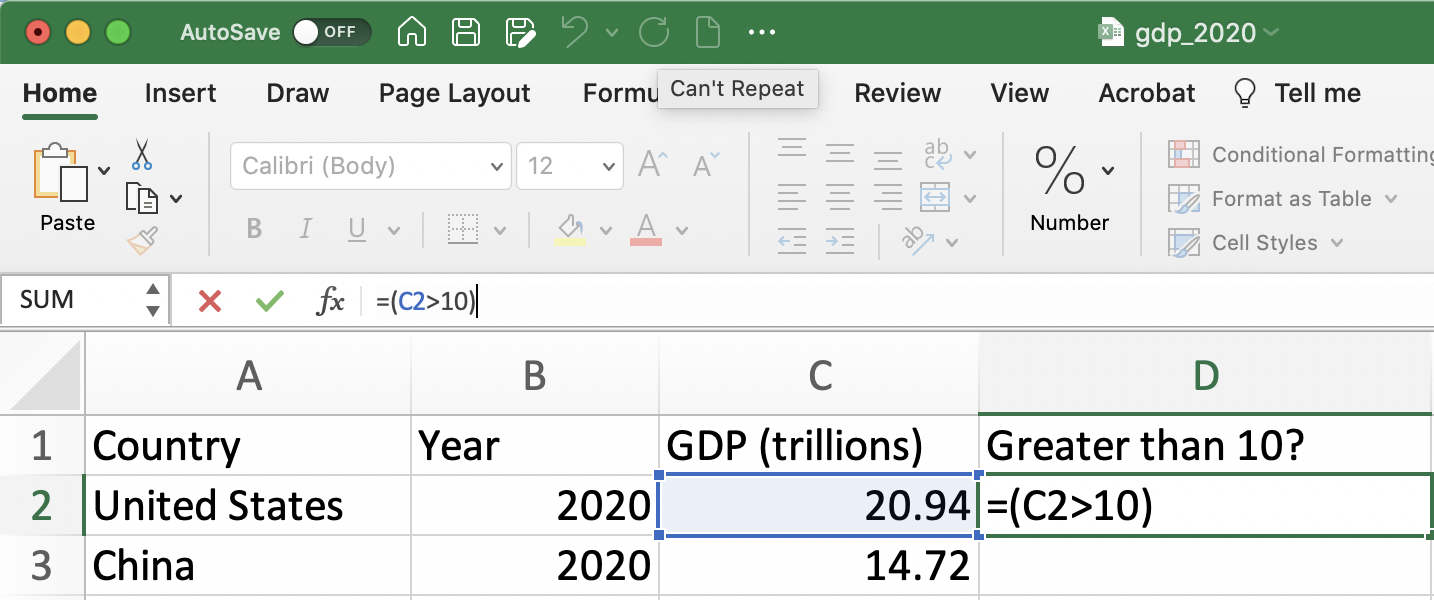
\includegraphics[width=1\linewidth]{images/01_tf1} 

}

\caption{Is GDP Greater than 10 in the U.S. Part 1}\label{fig:tf1}
\end{figure}

Once we press enter, we will get the result. In this case, we can see GDP in the U.S. is indeed greater than 10 trillion dollars. Therefore, when the function in cell D2 is evaluated it returns the answer \texttt{TRUE} as can be seen in Figure \ref{fig:tf2}.

\begin{figure}

{\centering 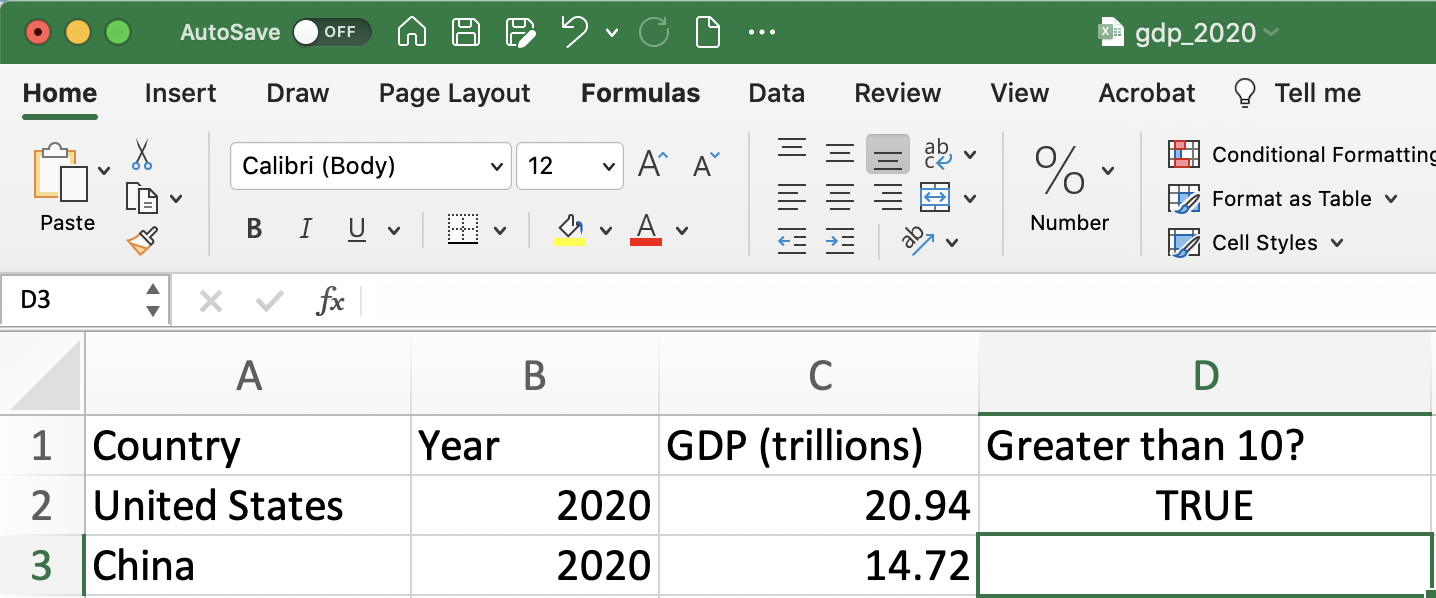
\includegraphics[width=1\linewidth]{images/01_tf2} 

}

\caption{Is GDP Greater than 10 in the U.S. Part 2}\label{fig:tf2}
\end{figure}

Once we have filled in the formula for one cell, we can also apply it to the remaining observations. In our example, this would mean testing whether each country's GDP is more than 10, not just the U.S. There are a couple of ways to do this efficiently in Excel.

One way to fill in the formula is to click the bottom right corner of cell D2 and then drag down. This allows you to apply to as many observations as you would like. However, we often want to apply the logical statement to all observations. Therefore, continuously dragging will be inefficient if there are thousands of observations in the data. To quickly apply a formula to all cells in a column, we can simply double click the bottom right corner of a cell. In our example, this would mean double clicking the bottom right corner of the D2 cell.

\begin{figure}

{\centering 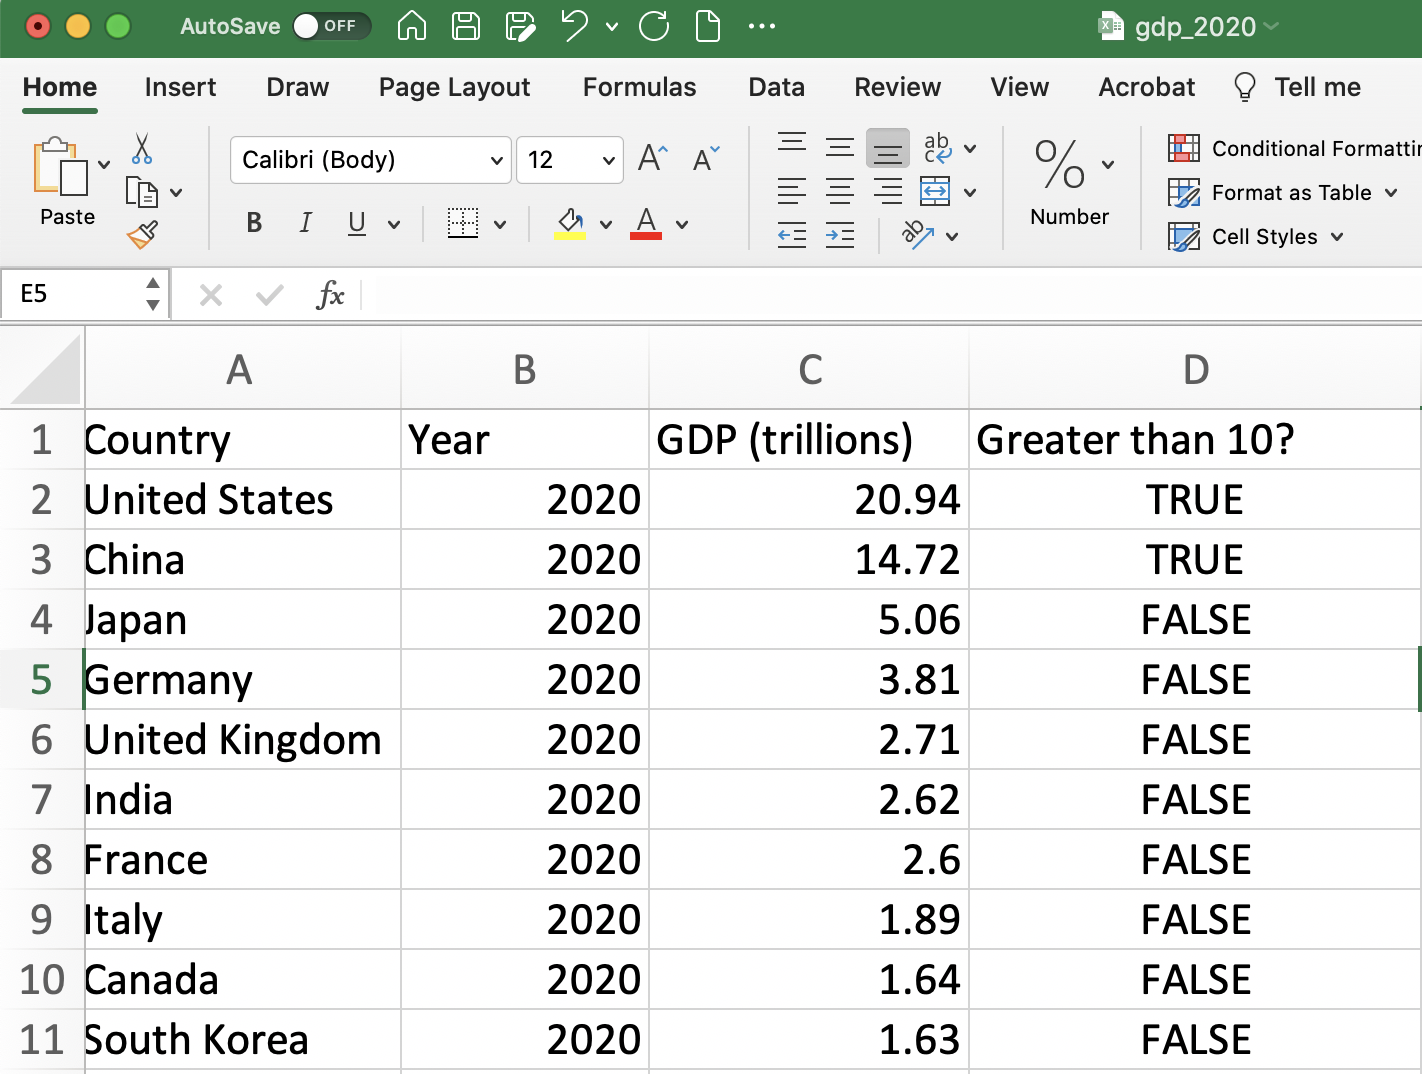
\includegraphics[width=1\linewidth]{images/01_fill} 

}

\caption{Filling in the Formula}\label{fig:fill}
\end{figure}

Oftentimes, instead of returning ``TRUE'' or ``FALSE'', it is convenient to have Excel return the value in another form. For example, a common way to represent ``TRUE'' is with the number 1 and ``FALSE'' with the number 0. To accomplish this in Excel we will use the \texttt{IF} function.

The basic format for the \texttt{IF} function is:

\begin{center}
\colorbox{gray!20}{\texttt{=IF(logical test,value if TRUE, value if FALSE)}}
\end{center}

For example, in our dataset, if we want to return the value of 1 if GDP is greater than 10 and 0 if otherwise, we can type:

\begin{center}
\colorbox{gray!20}{\texttt{=IF(C2>10,1,0)}}
\end{center}

\begin{figure}

{\centering 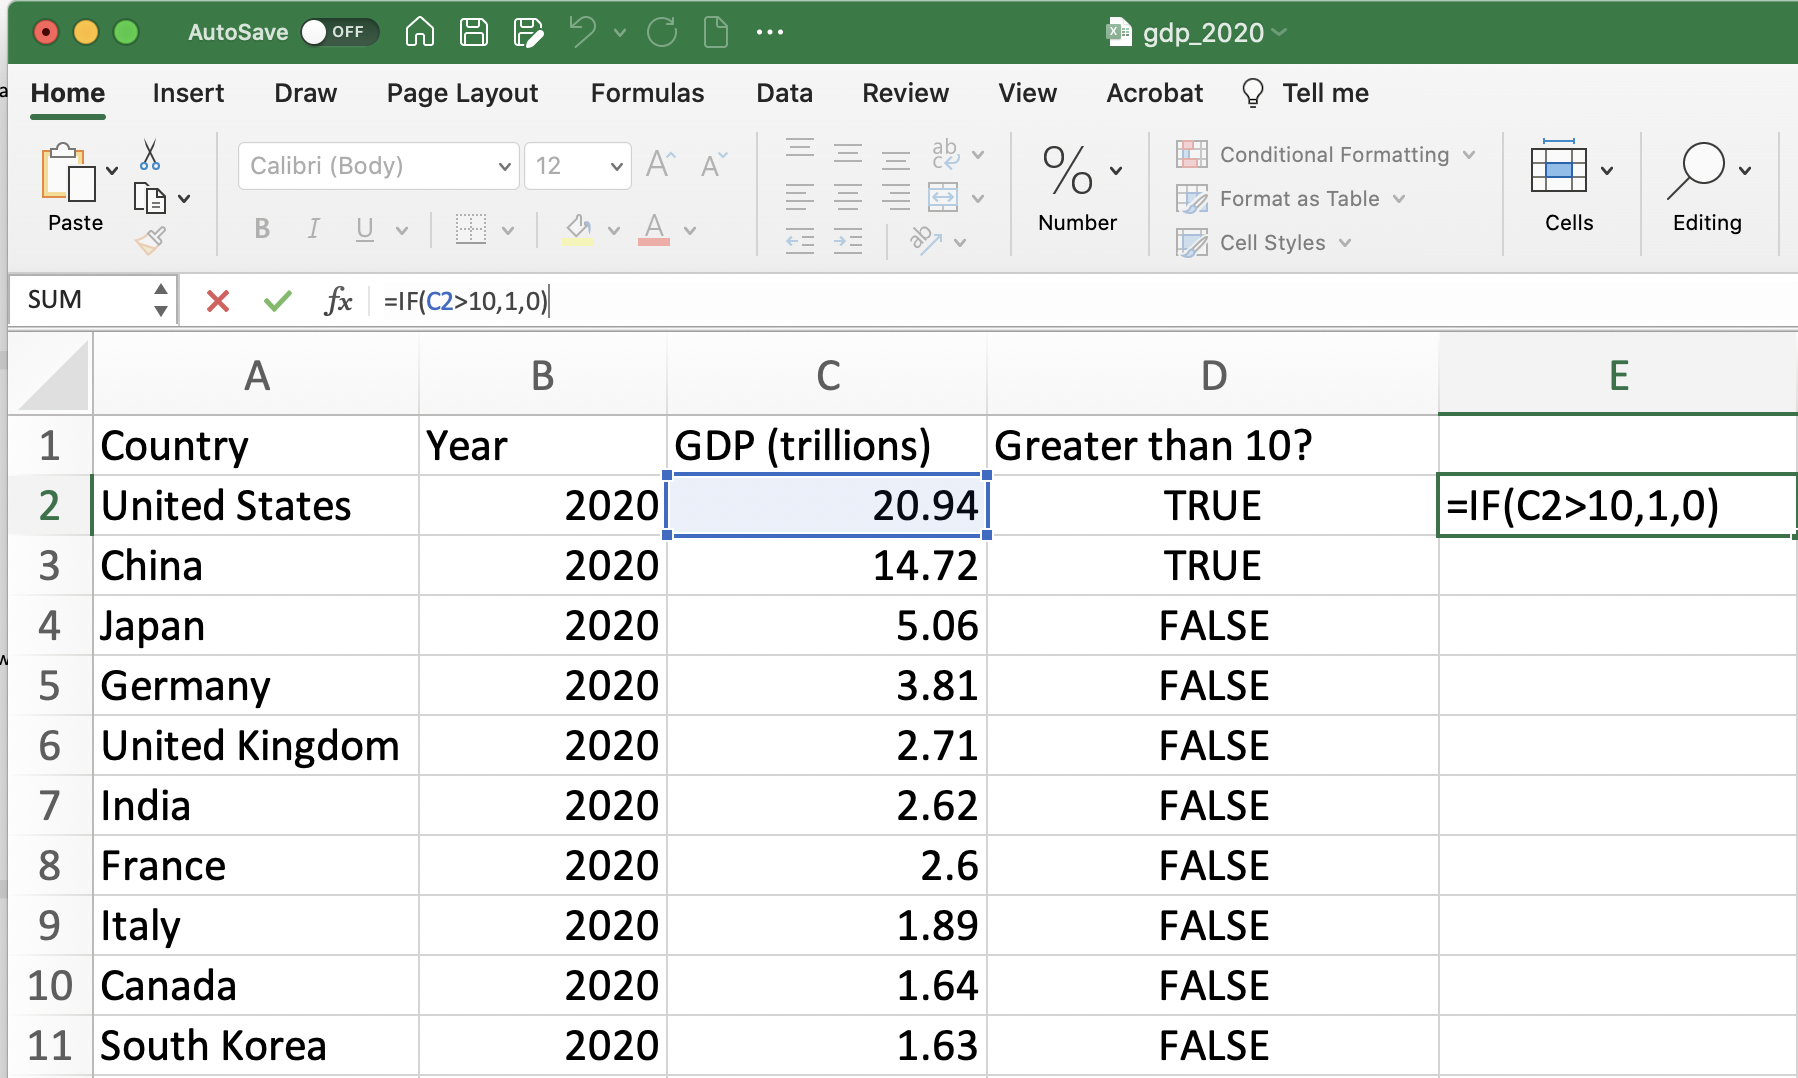
\includegraphics[width=1\linewidth]{images/01_if1} 

}

\caption{Using the IF function (Before Pressing Enter)}\label{fig:ifex1}
\end{figure}

Once we press enter, the function is evaluated. To fill in the formula for the rest of the observations you can follow the same steps as above.

\begin{figure}

{\centering 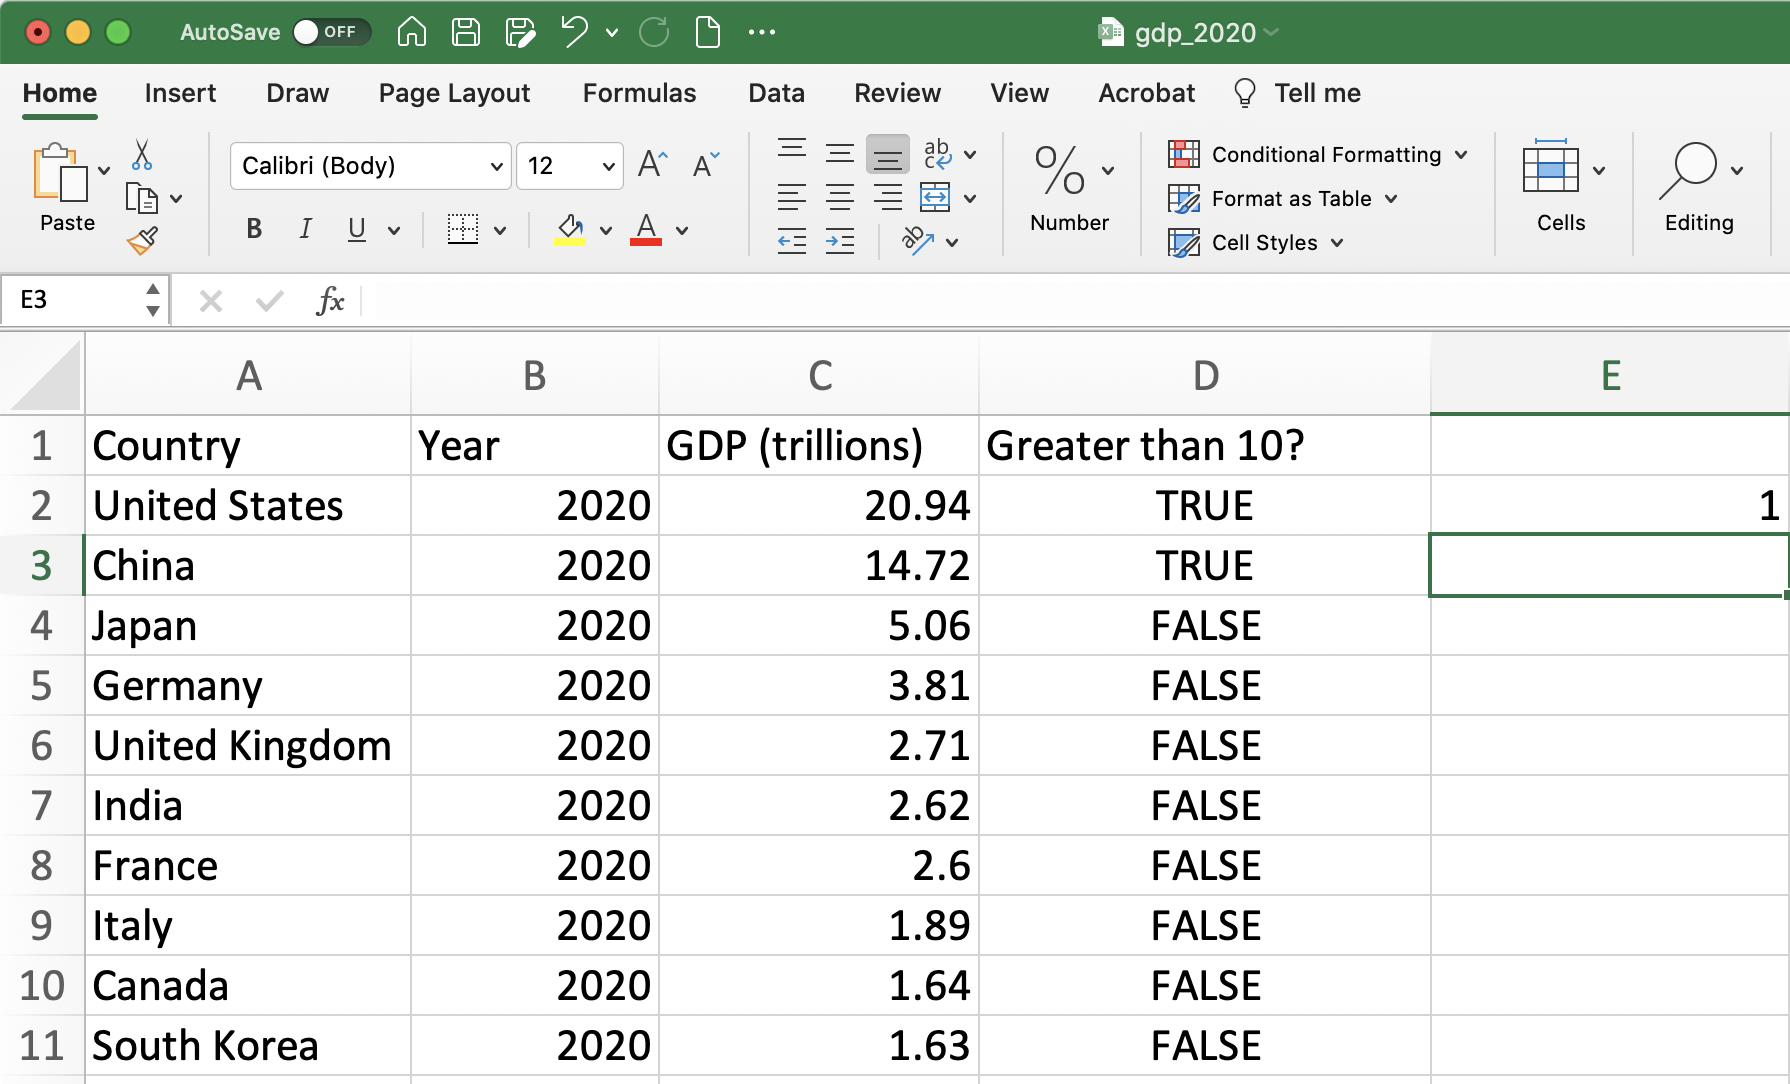
\includegraphics[width=1\linewidth]{images/01_if2} 

}

\caption{Using the IF function (After Pressing Enter)}\label{fig:ifex2}
\end{figure}

\hypertarget{summary-statistics}{%
\section{Summary Statistics}\label{summary-statistics}}

Now let's return to our data from Brownback and Sadoff (2020). Our goal is to create a table of basic summary statistics. However, a key variable in the Brownback and Sadoff (2020) experiment is whether a given student passed the test or not. This financial compensation of an instructor (in the treatment group) directly depends on how many students pass the test. This currently does not appear in our dataset, so we will have to create it.

To create this variable we need to take three steps:

\begin{itemize}
\item
  \textbf{First Step:} Title the column with the variable name ``Passed''
\item
  \textbf{Second Step:} Use the \texttt{IF} function to fill in this variable for the first observation
\item
  \textbf{Third Step:} Double click bottom right of cell in step 2 to fill in the variable for all observations
\end{itemize}

Figure \ref{fig:passed1} presents steps 1 and 2 in Excel.

\begin{figure}

{\centering 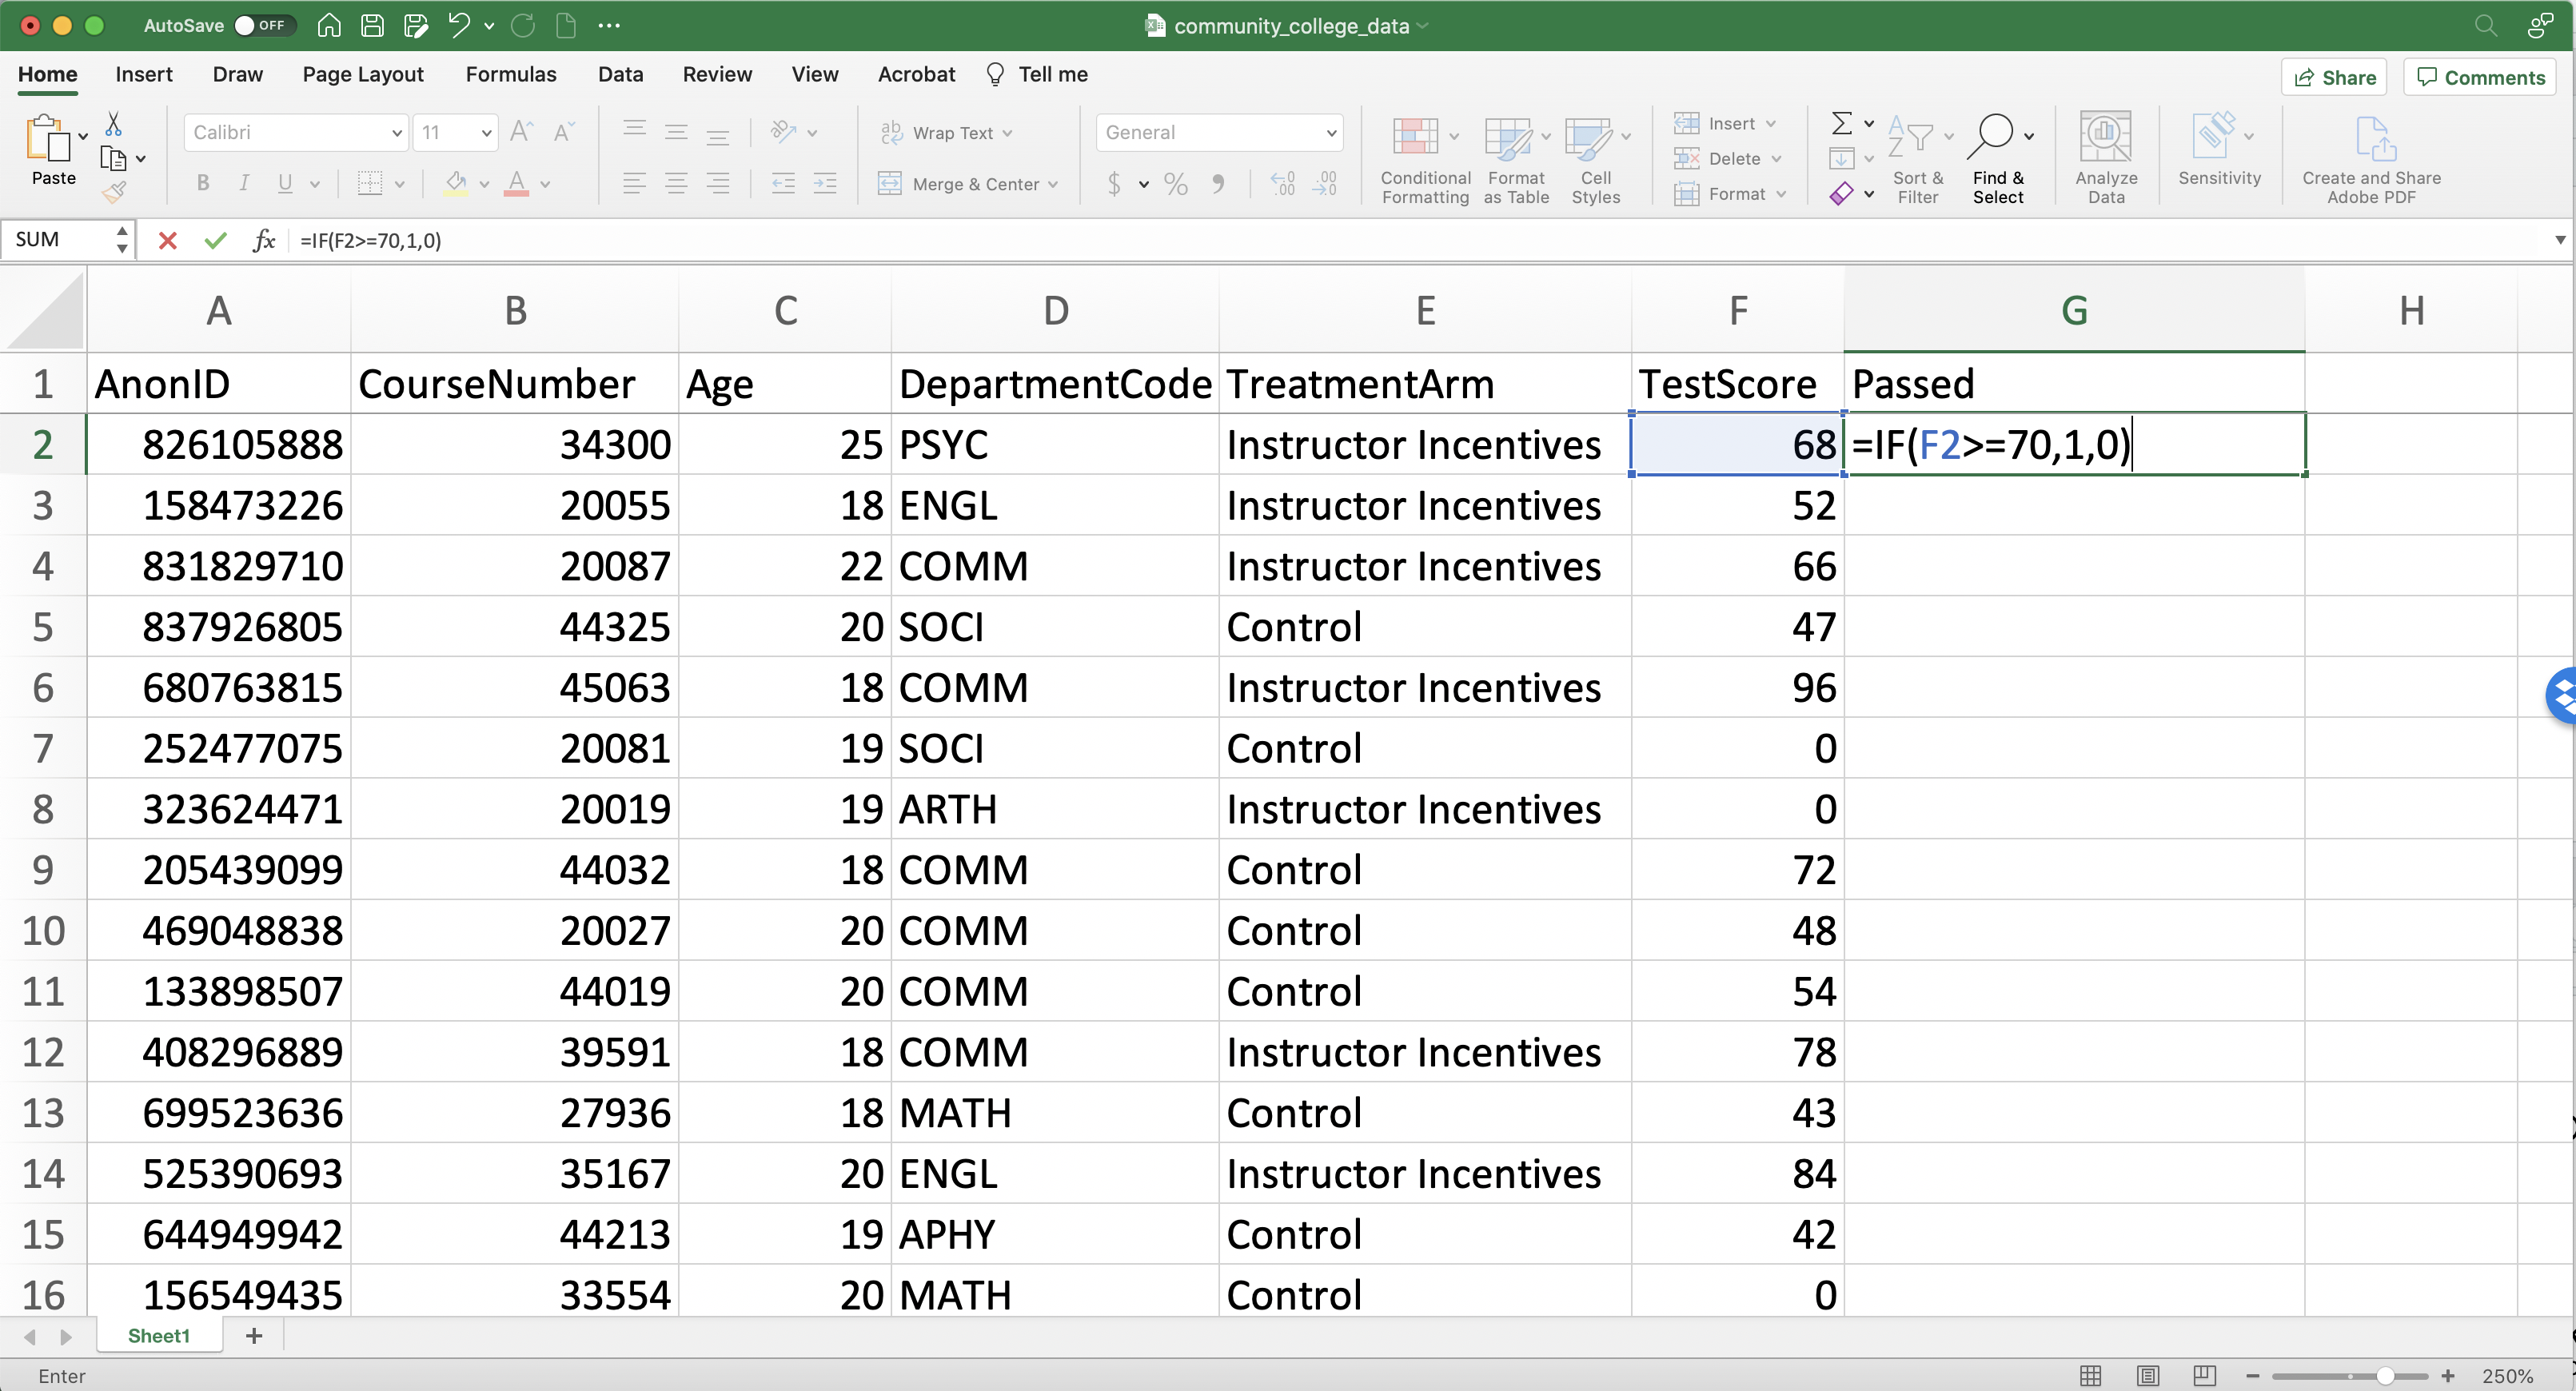
\includegraphics[width=1\linewidth]{images/01_passed1} 

}

\caption{Generating a Passed Variable (Steps 1 and 2)}\label{fig:passed1}
\end{figure}

We simply can double click the bottom right of G2 to fill in the rest of the observations (as seen in Figure \ref{fig:passed2}).

\begin{figure}

{\centering 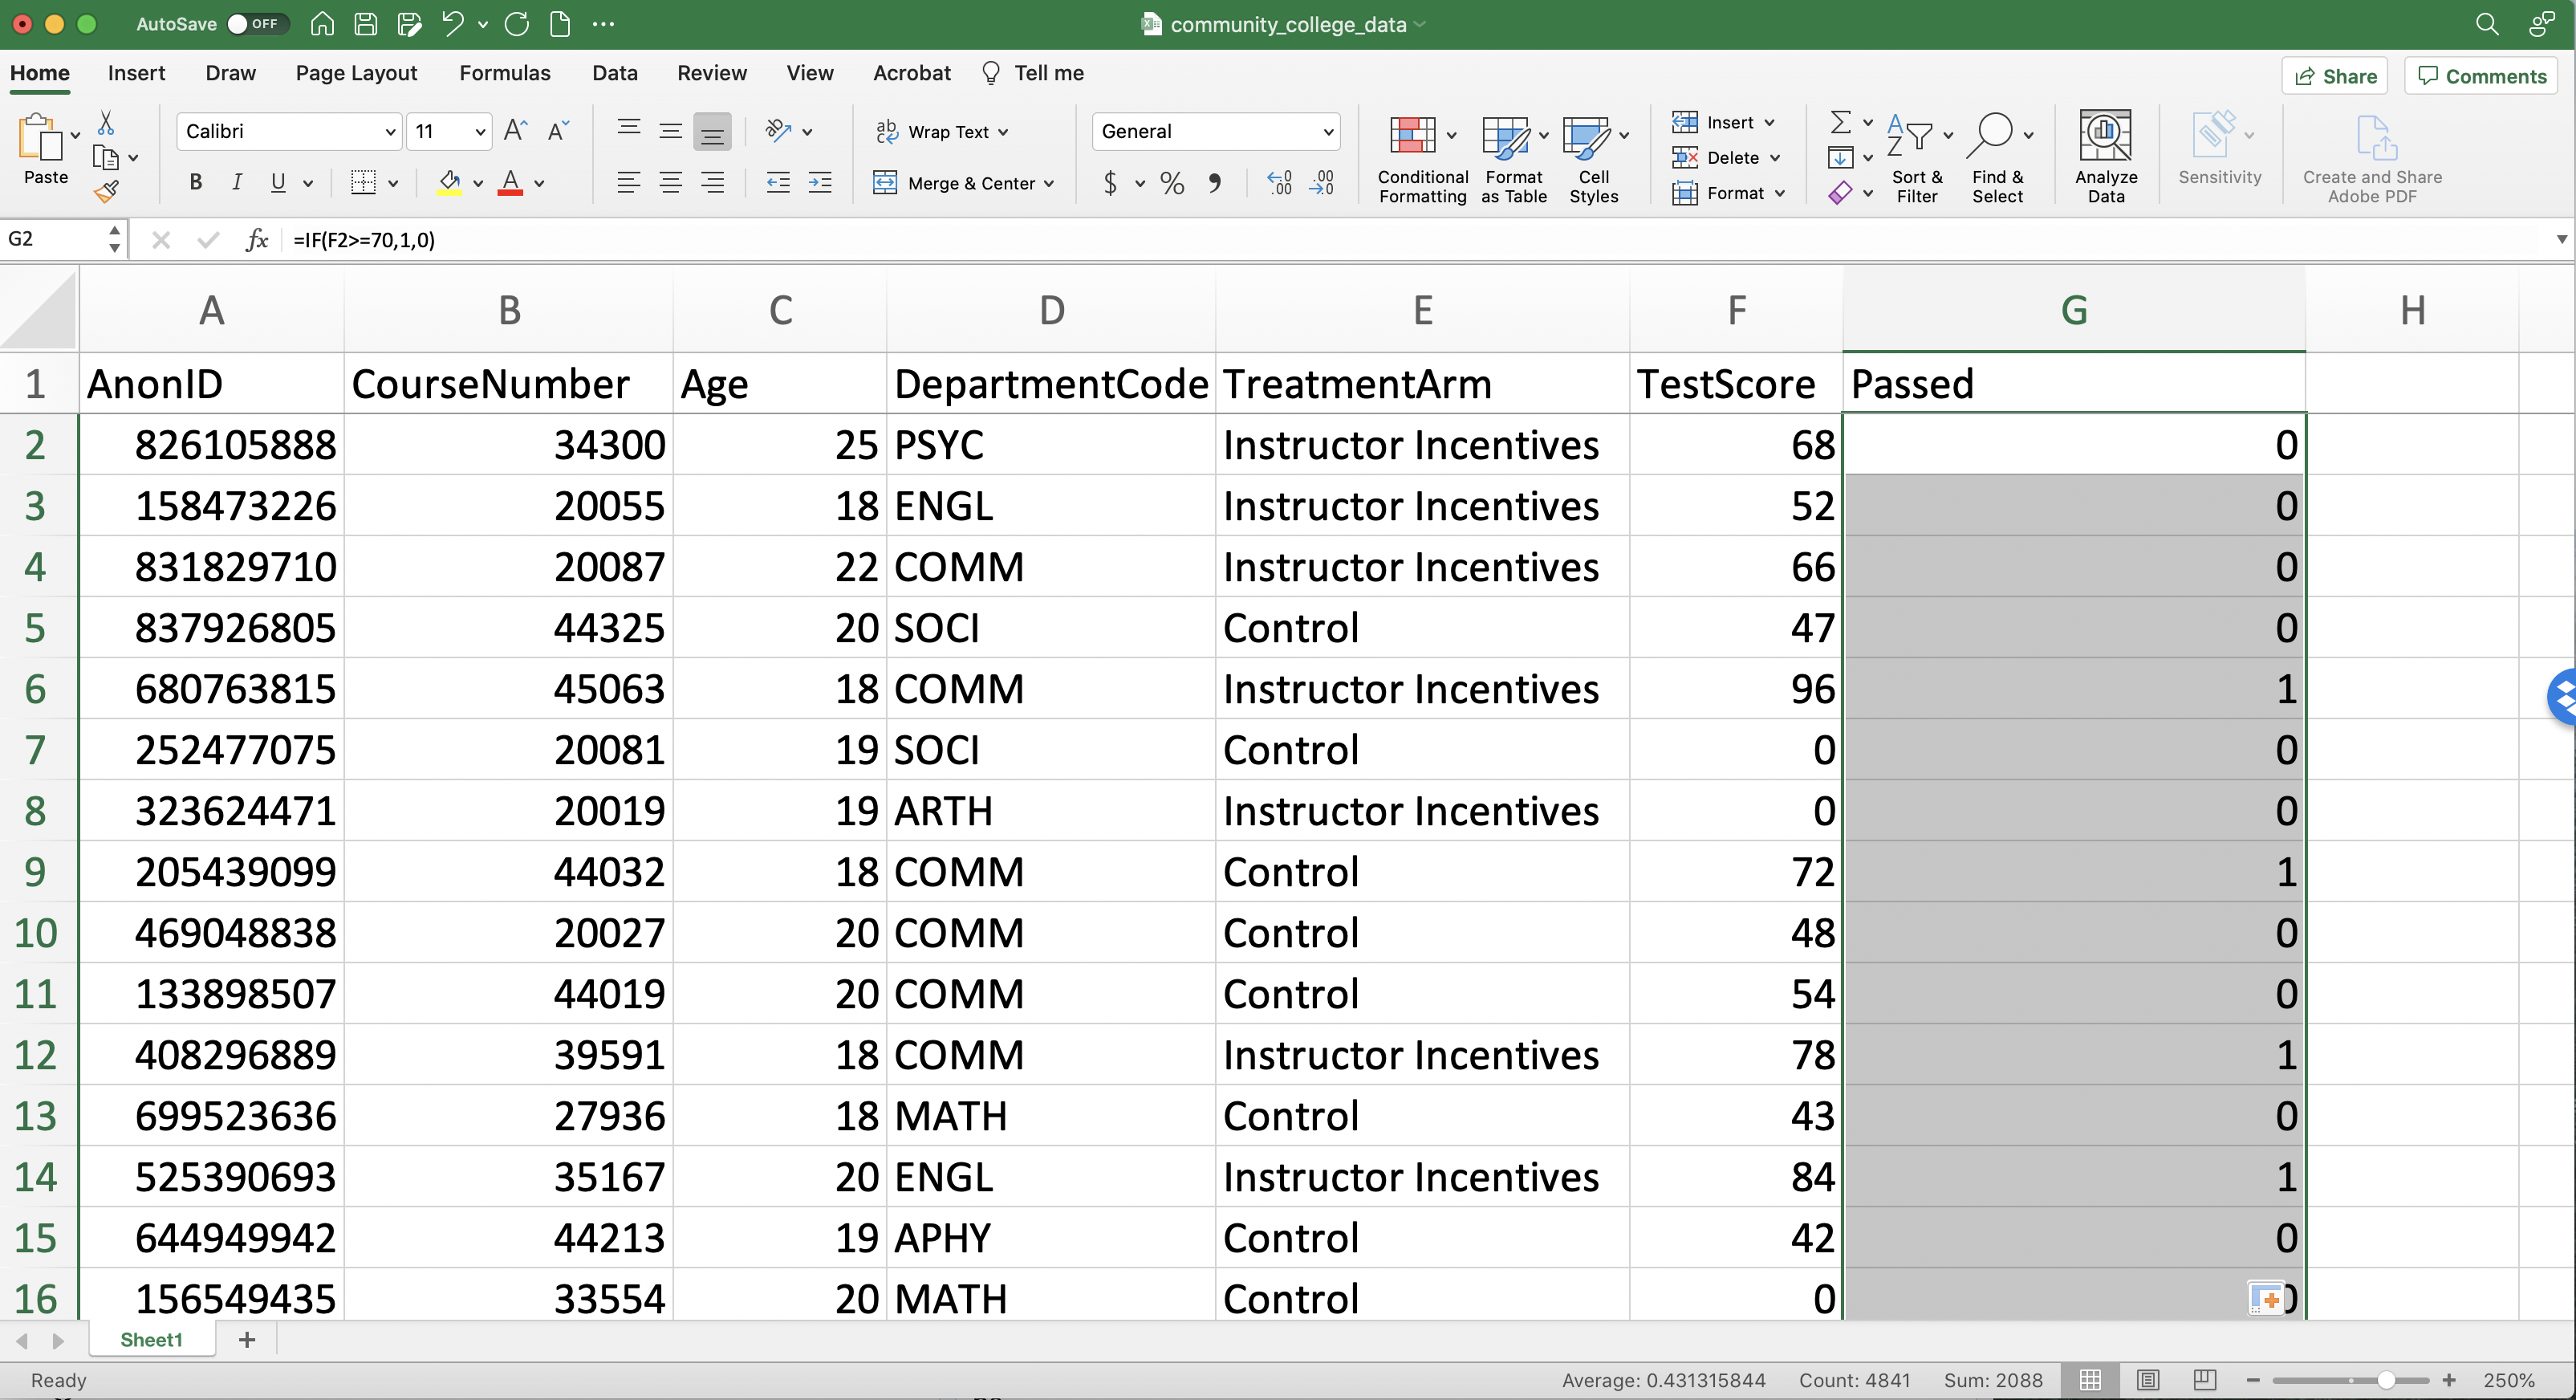
\includegraphics[width=1\linewidth]{images/01_passed2} 

}

\caption{Generating a Passed Variable (Step 3)}\label{fig:passed2}
\end{figure}

Now that we've generated the variables we need let's fill in some summary statistics displayed on the right side of the datasheet in Figure \ref{fig:sumstats1}

\begin{figure}

{\centering 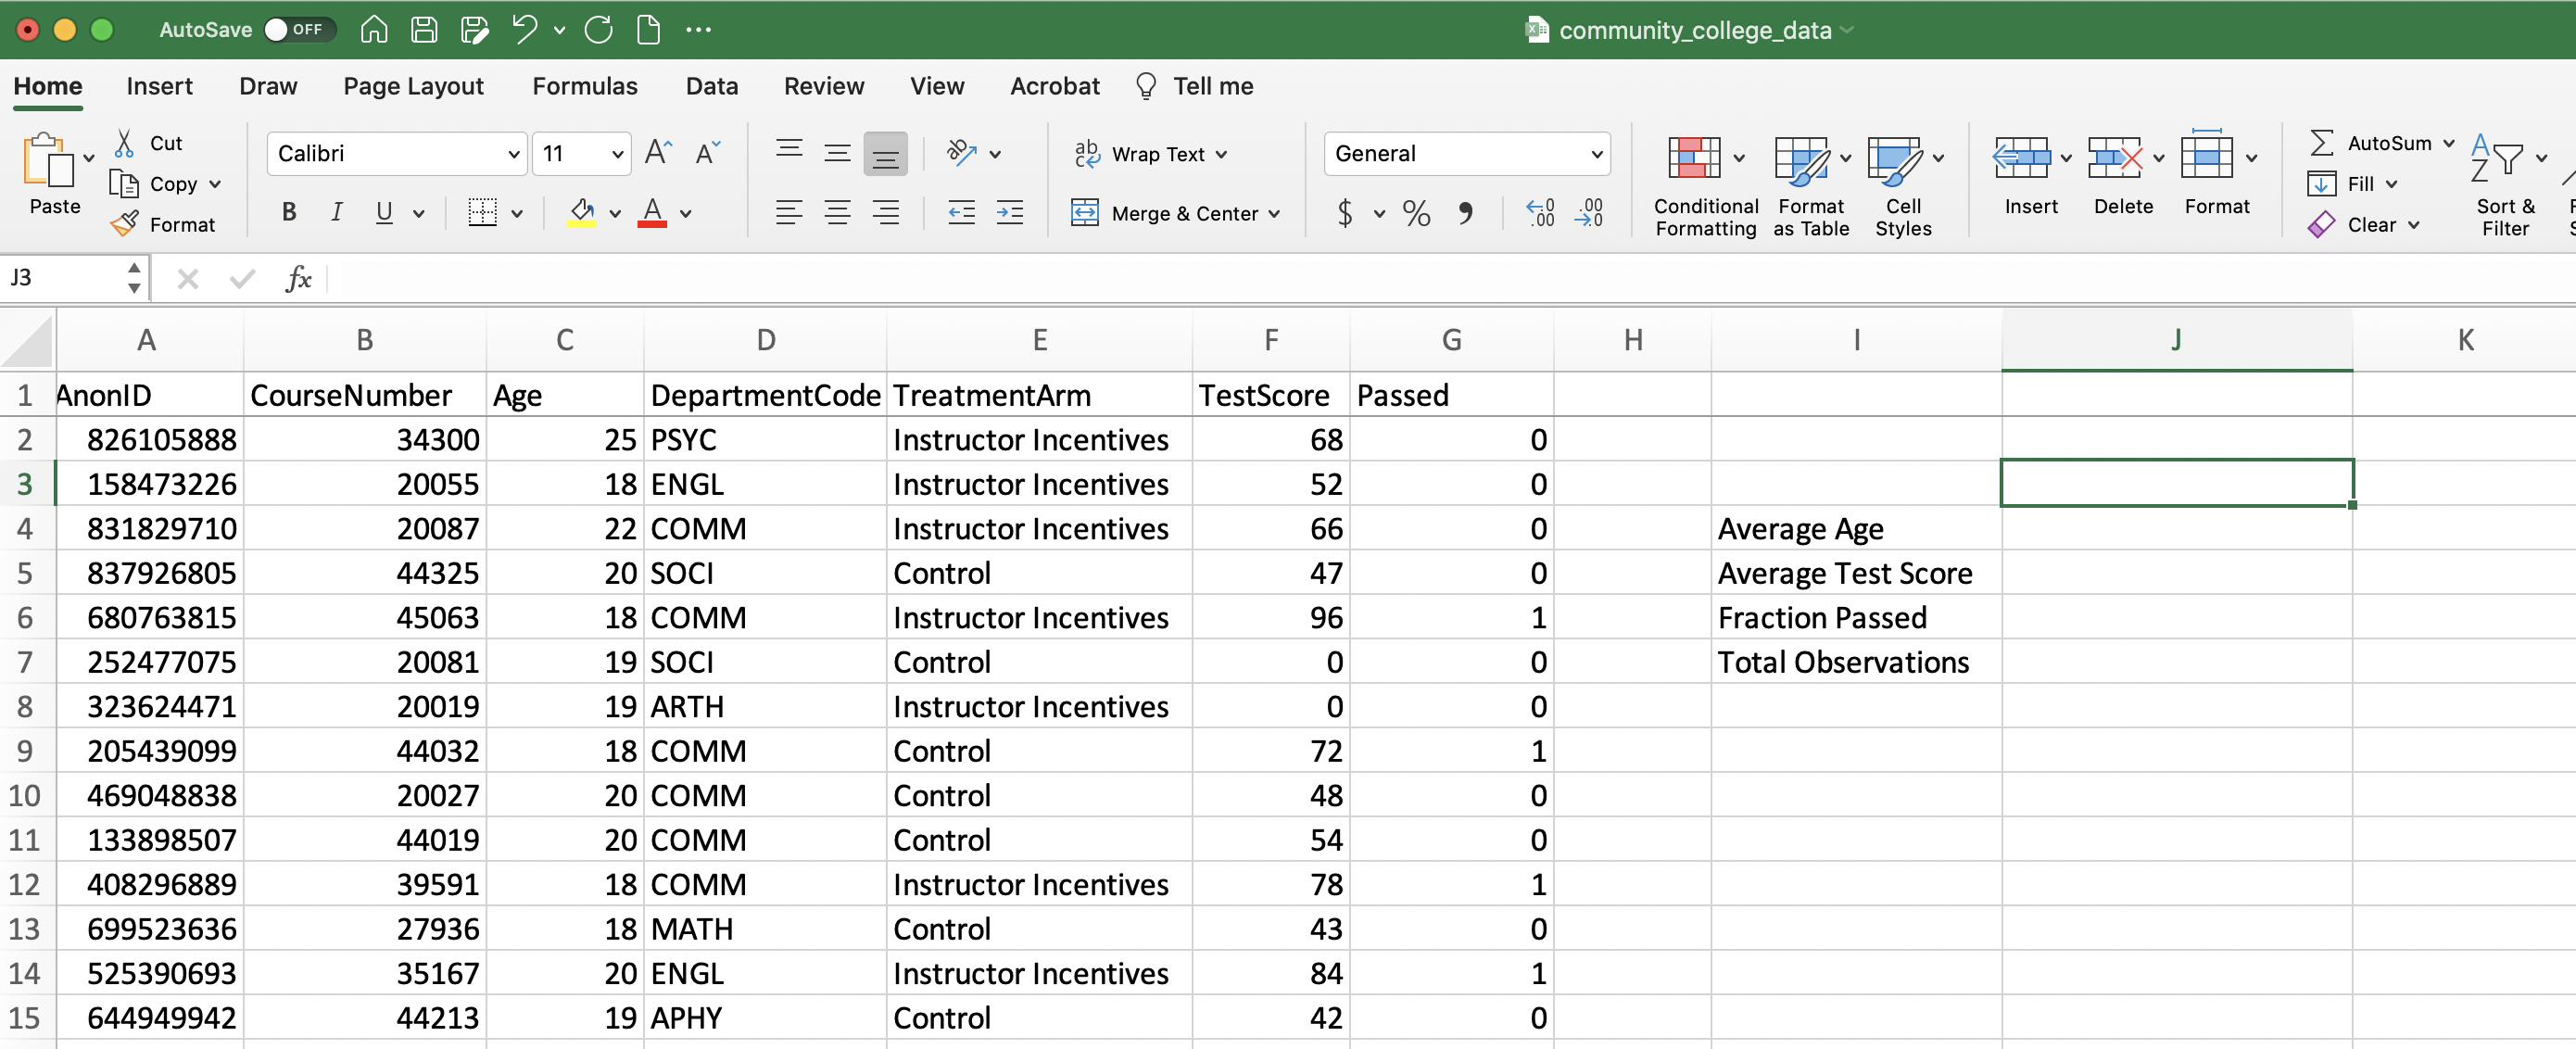
\includegraphics[width=1\linewidth]{images/01_sumstats1} 

}

\caption{Blank Summary Statistics Table}\label{fig:sumstats1}
\end{figure}

To compute average age in the dataset we just need to use the \texttt{AVERAGE} function and reference column C.

\begin{figure}

{\centering 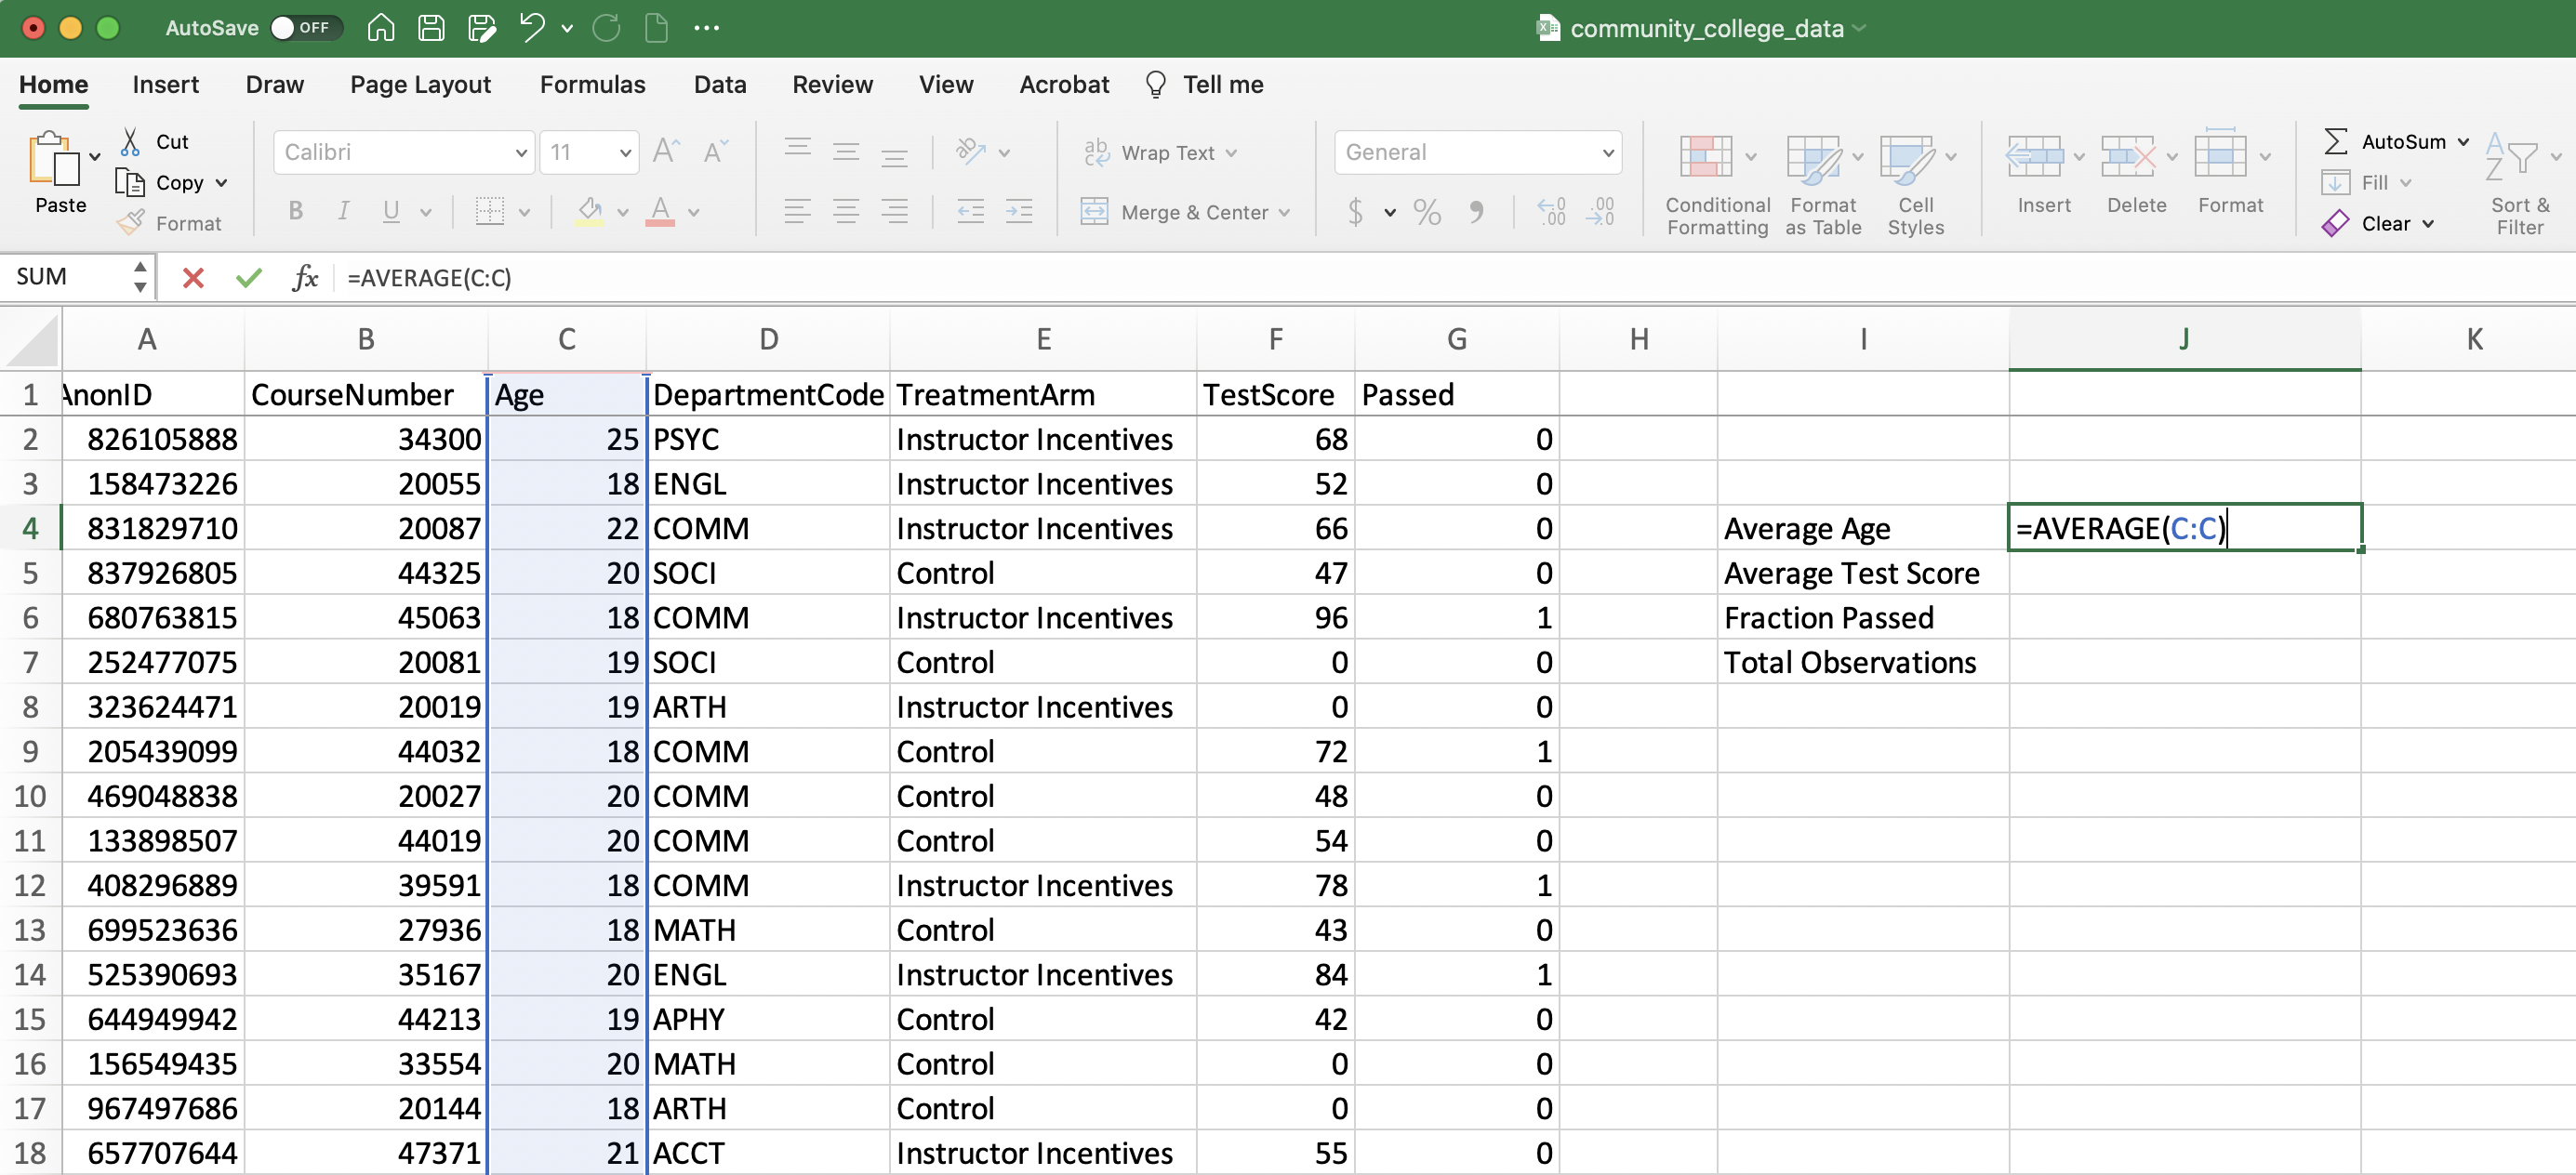
\includegraphics[width=1\linewidth]{images/01_sumstats2} 

}

\caption{Average Age}\label{fig:sumstats2}
\end{figure}

Average test score is completely analogous to age, but we now reference column F.

\begin{figure}

{\centering 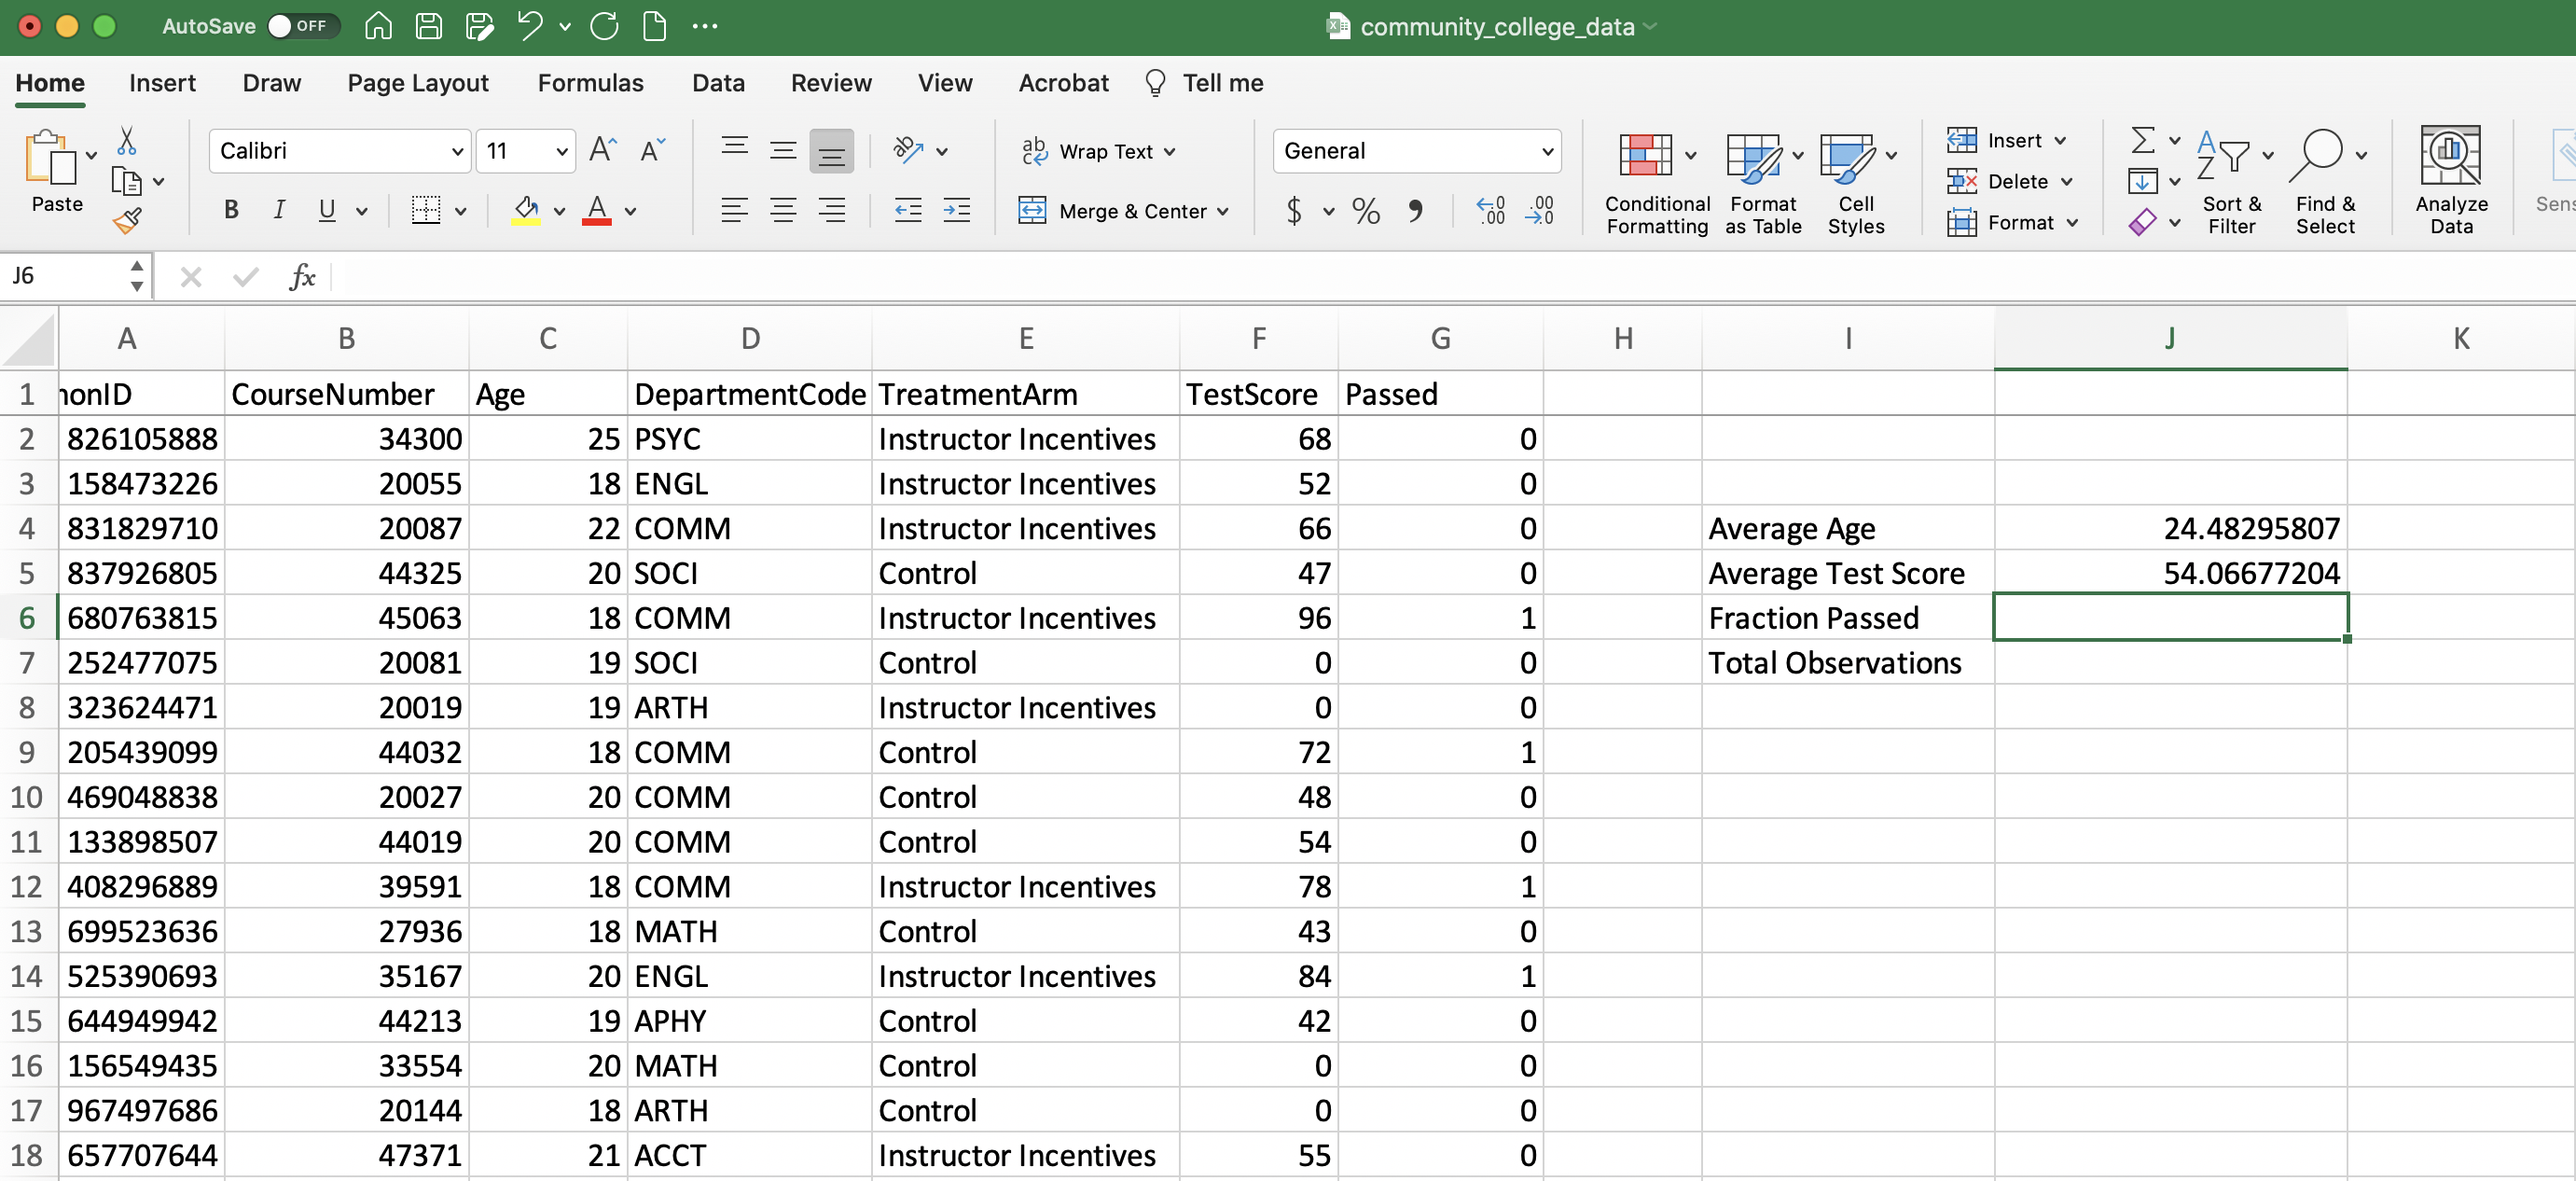
\includegraphics[width=1\linewidth]{images/01_sumstats3} 

}

\caption{Average Test Score}\label{fig:sumstats3}
\end{figure}

In order to compute fraction that passed the test, we are going to make a small digression, one that will clarify one reason it was convenient to store the variable Passed with a 1 if the individual passed and a zero otherwise. Because we have stored the variable in this way, we can simply take the average value of Passed and this will be equal to the fraction that passed the test.

To see why this is true, let's first write out the equation for the average of a generic variable \(X\)

\[
  \bar{X} = \frac{X_1 + ... + X_N}{N} 
\]

Where \(N\) is the number of observations, \(X_1\) is the first observation and \(X_N\) is the \(N^{th}\) observation. If \(X\) is a binary variable that is equal to 1 or zero, then the average will be the fraction of individual's with a 1
\[
  \bar{X} = \frac{X_1 + ... + X_N}{N}=\frac{\text{Number of observations =1 }}{\text{Total Observations}} 
\]
Since our variable ``Passed'' is equal to 1 if passed and zero otherwise, the fraction who passed is the average of our ``Passed'' variable. Therefore, in Excel we simply need to compute the average of the G column

\begin{figure}

{\centering 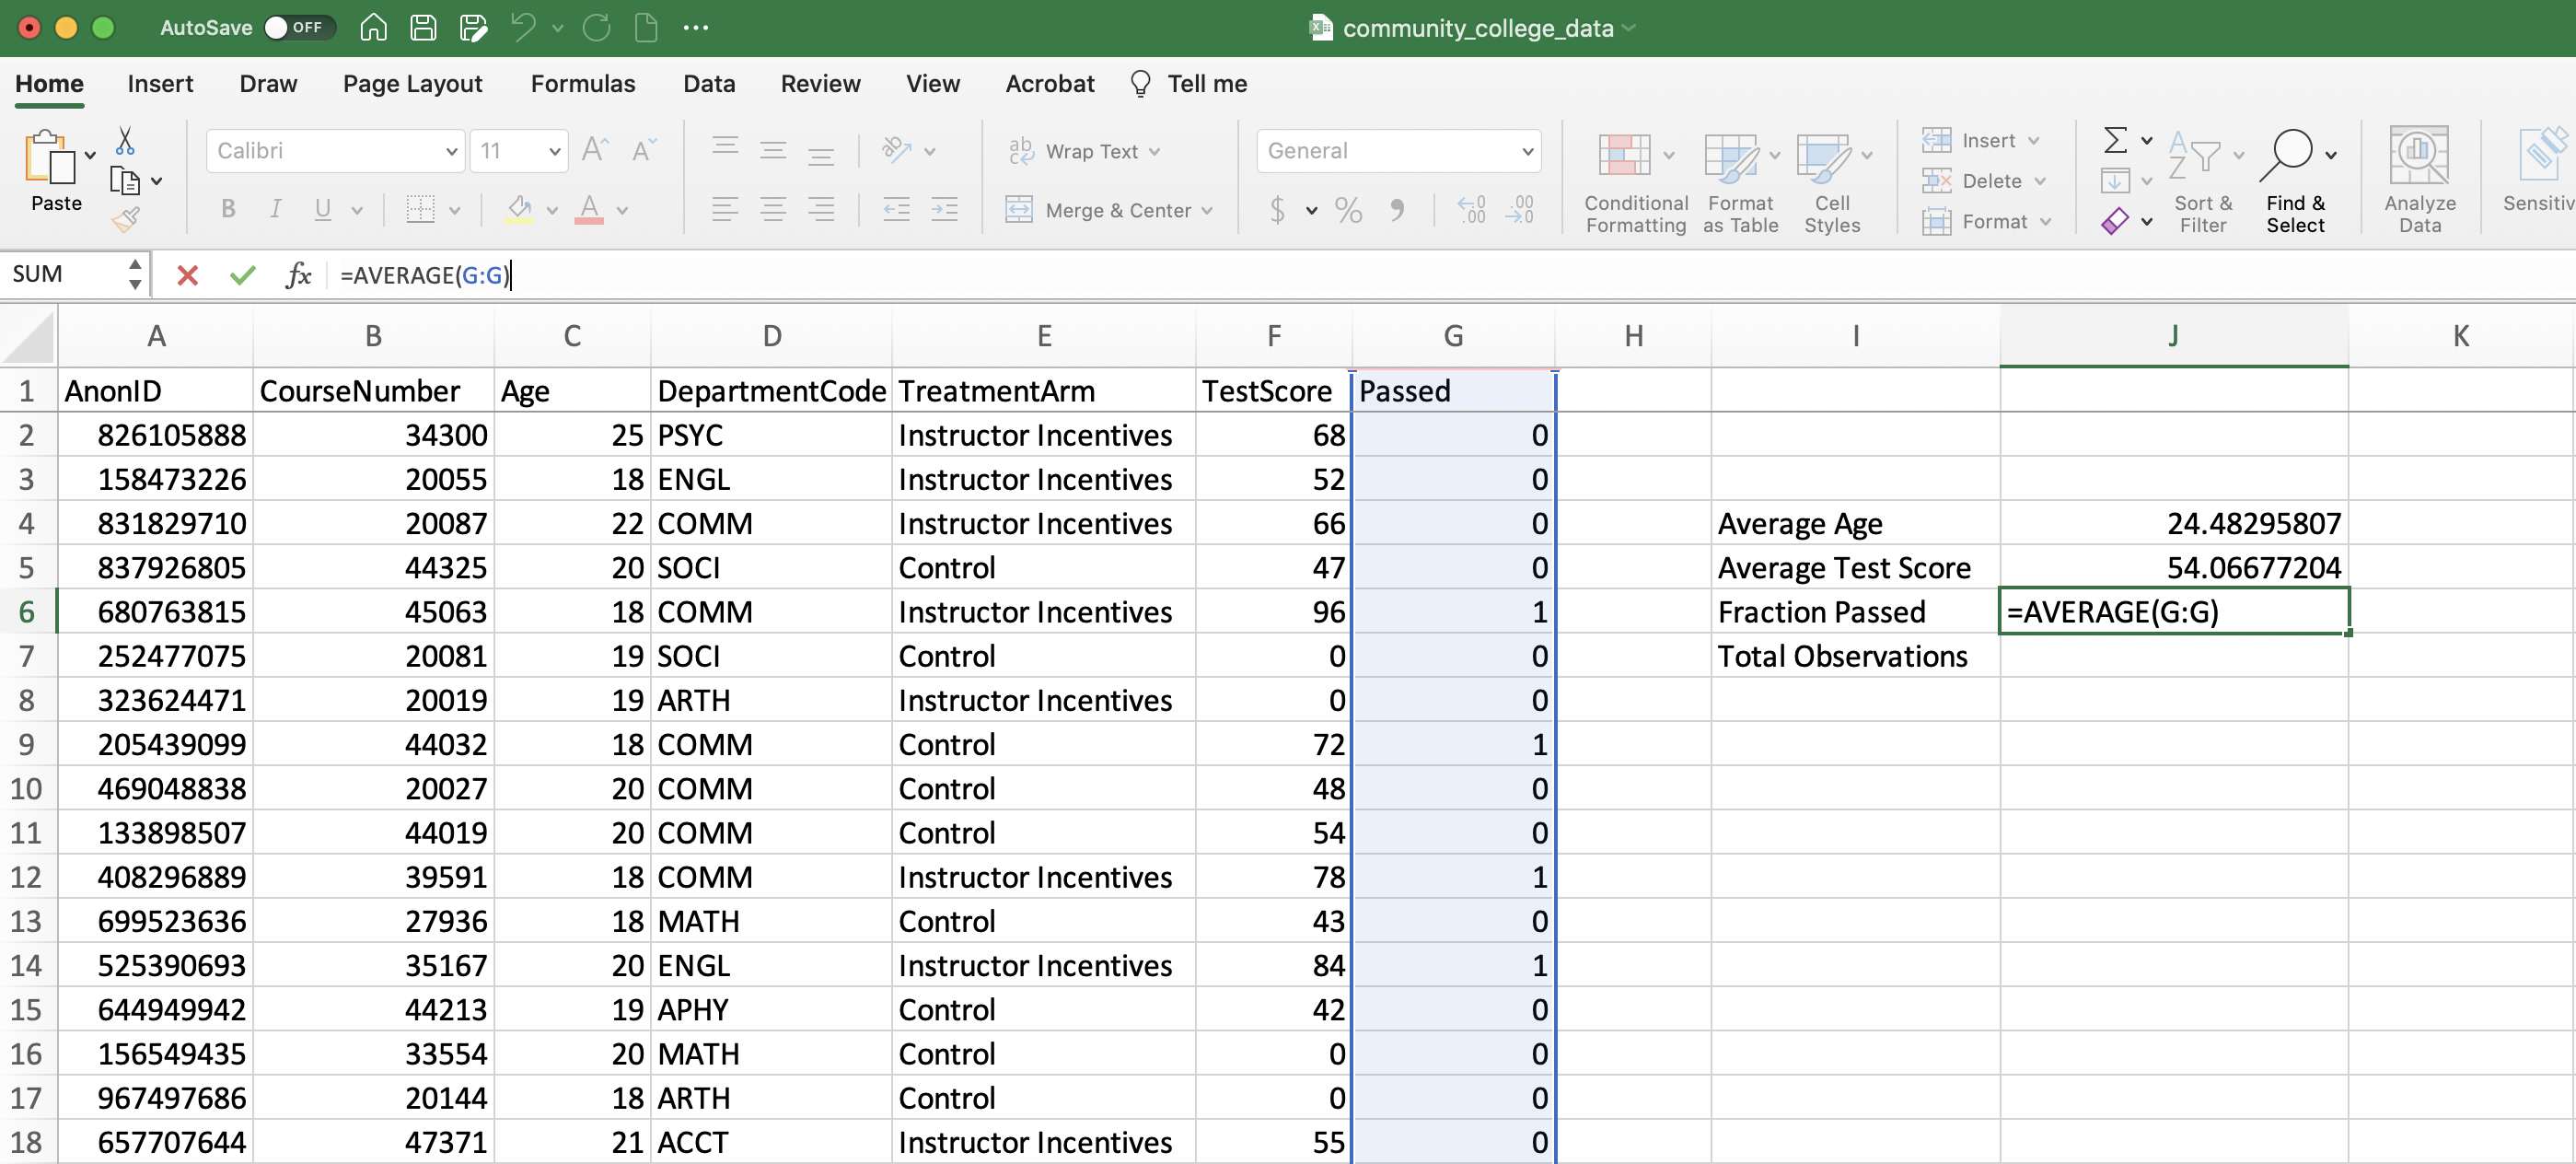
\includegraphics[width=1\linewidth]{images/01_frac_passed} 

}

\caption{Computing the Fraction Passed}\label{fig:fracpassed}
\end{figure}

Finally, to finish our summary statistics table, we need to fill in the total number of observations. To do this, we can use the \texttt{COUNT} function, which will count the total number of numbers in a column. While Figure \ref{fig:count} uses Column G to compute total observations, this could be replaced with any column that has non-missing numeric data.

\begin{figure}

{\centering 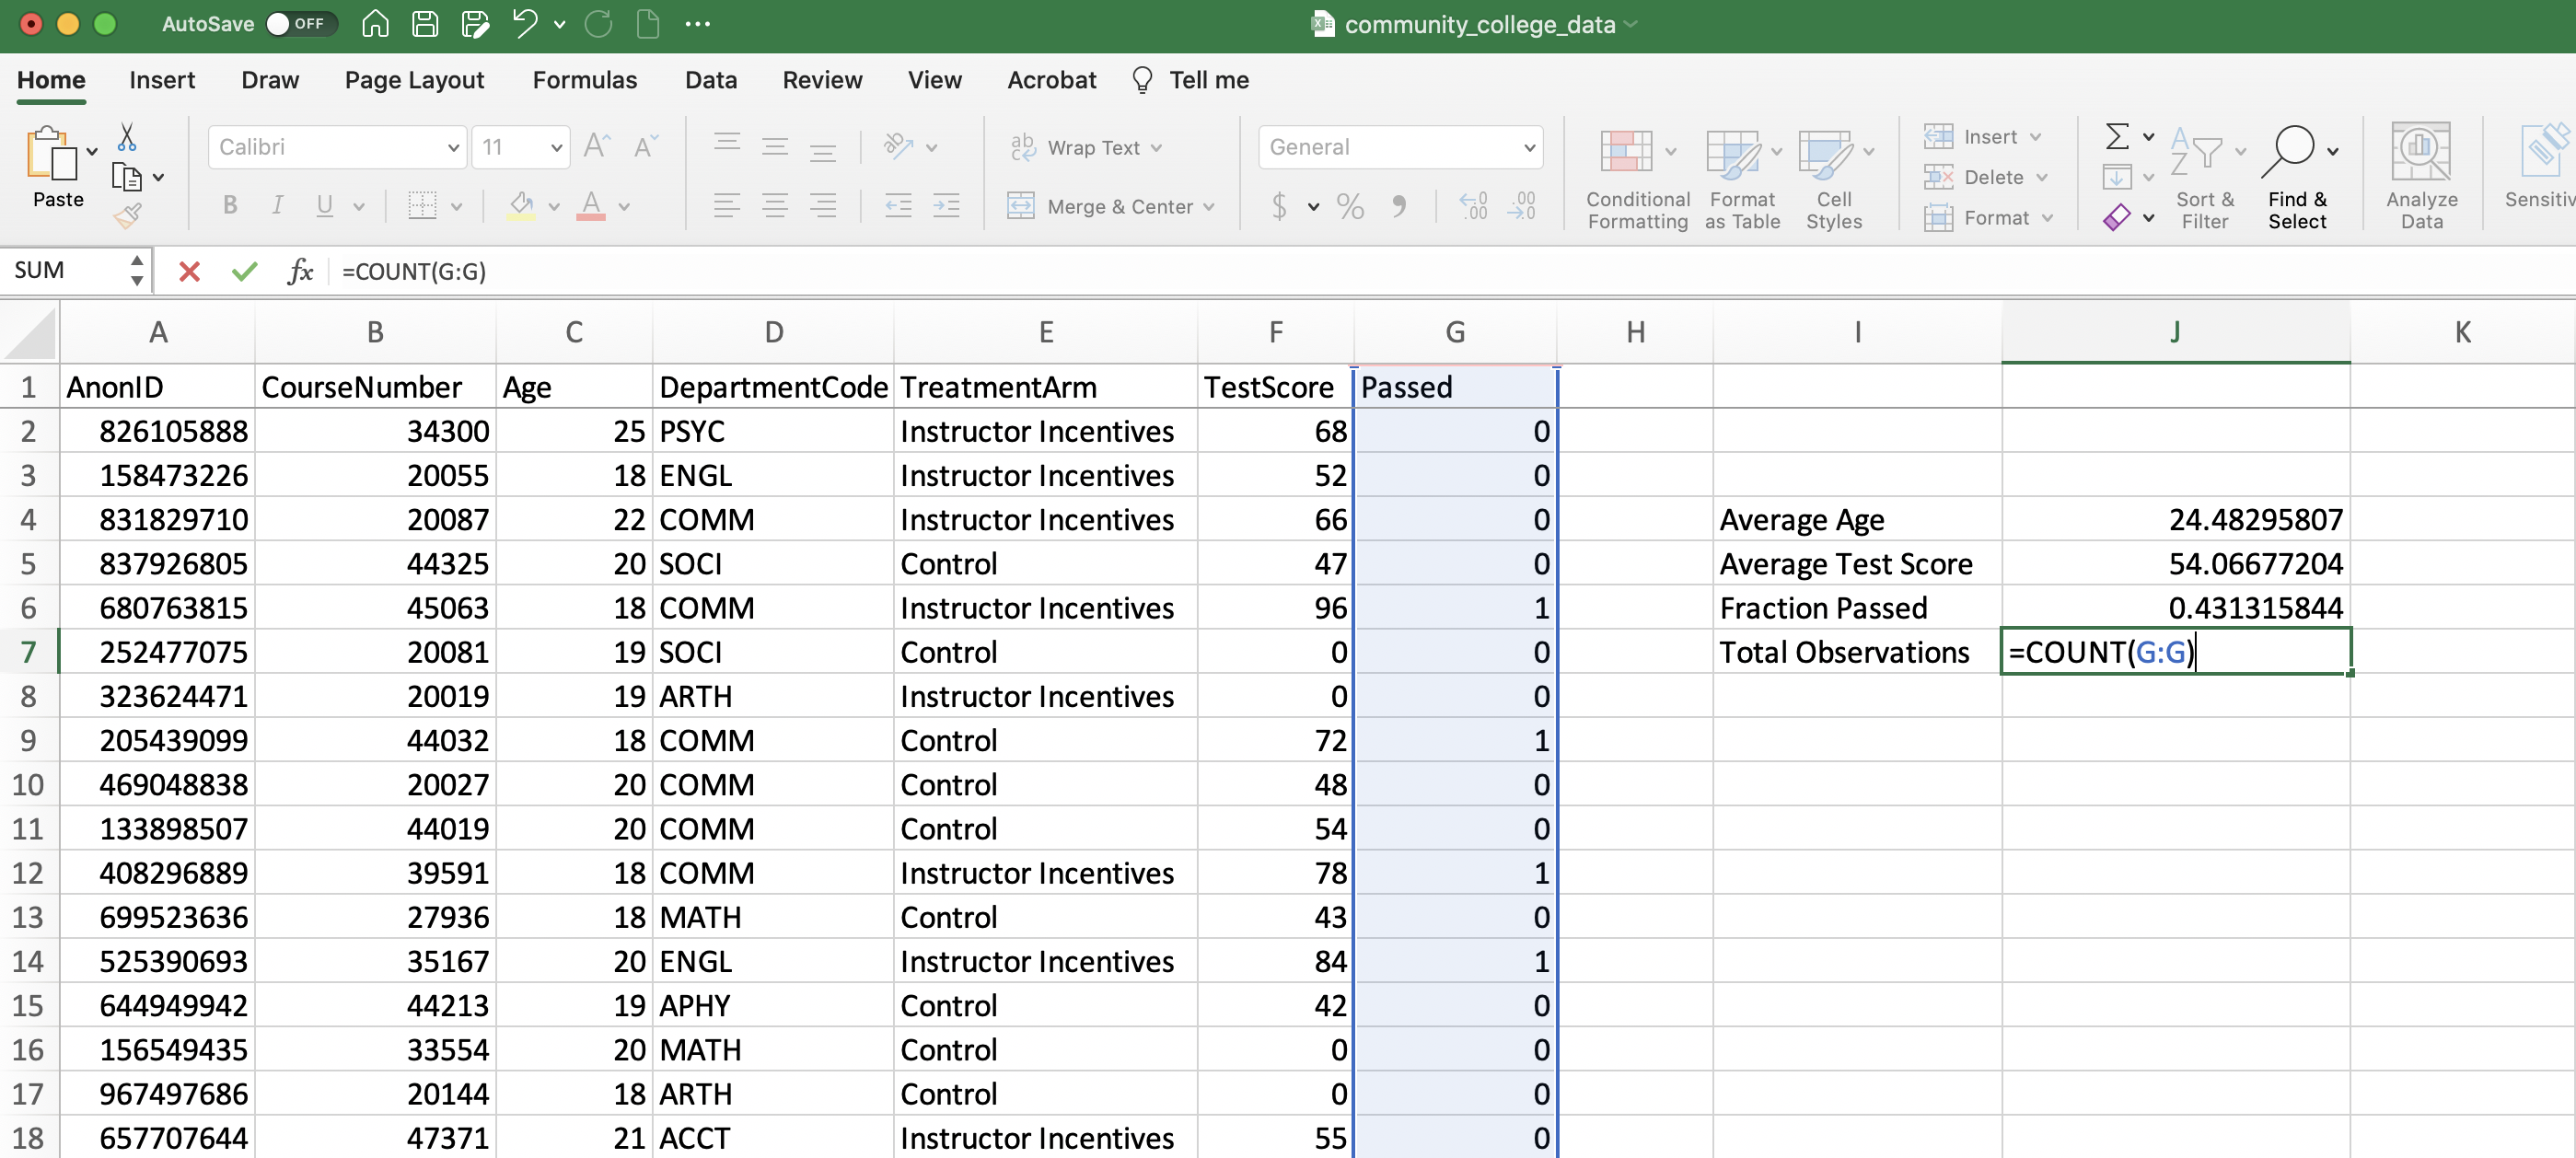
\includegraphics[width=1\linewidth]{images/01_count} 

}

\caption{Computing Total Observations}\label{fig:count}
\end{figure}

\hypertarget{heading.pivottables}{%
\section{Pivot Tables}\label{heading.pivottables}}

So far, we have learned to retrieve summary statistics using functions. This works very well for retrieving summary statistics for the entire dataset. Sometimes however we want more complicated summary statistics. For example, in our empirical application, we might be interested in passing rates for different departments. While it is possible to retrieve these using functions, an easier way is through a \textbf{pivot table}. The name ``pivot'' comes from ``pivoting'' the data into a way the provides useful information.

To understand what we are trying to accomplish with our pivot table, let's start by looking at our end goal in Figure \ref{fig:pivotfinal}. In the Pivot Table, each \textbf{row} is a separate department, with the fraction passed displayed.

\begin{figure}

{\centering 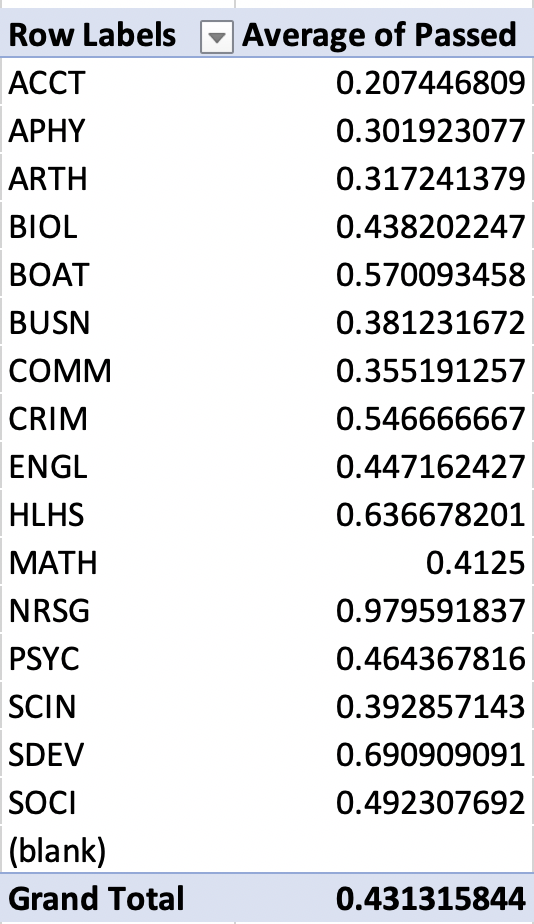
\includegraphics[width=0.38\linewidth]{images/01_pivot_final} 

}

\caption{Pivot Table: Pass Rates by Department}\label{fig:pivotfinal}
\end{figure}

Now let's go through how to construct Figure \ref{fig:pivotfinal}. To insert a pivot table, go to the Insert tab and click ``Insert Pivot Table'', as seen in Figure \ref{fig:pivot1}

\begin{figure}

{\centering 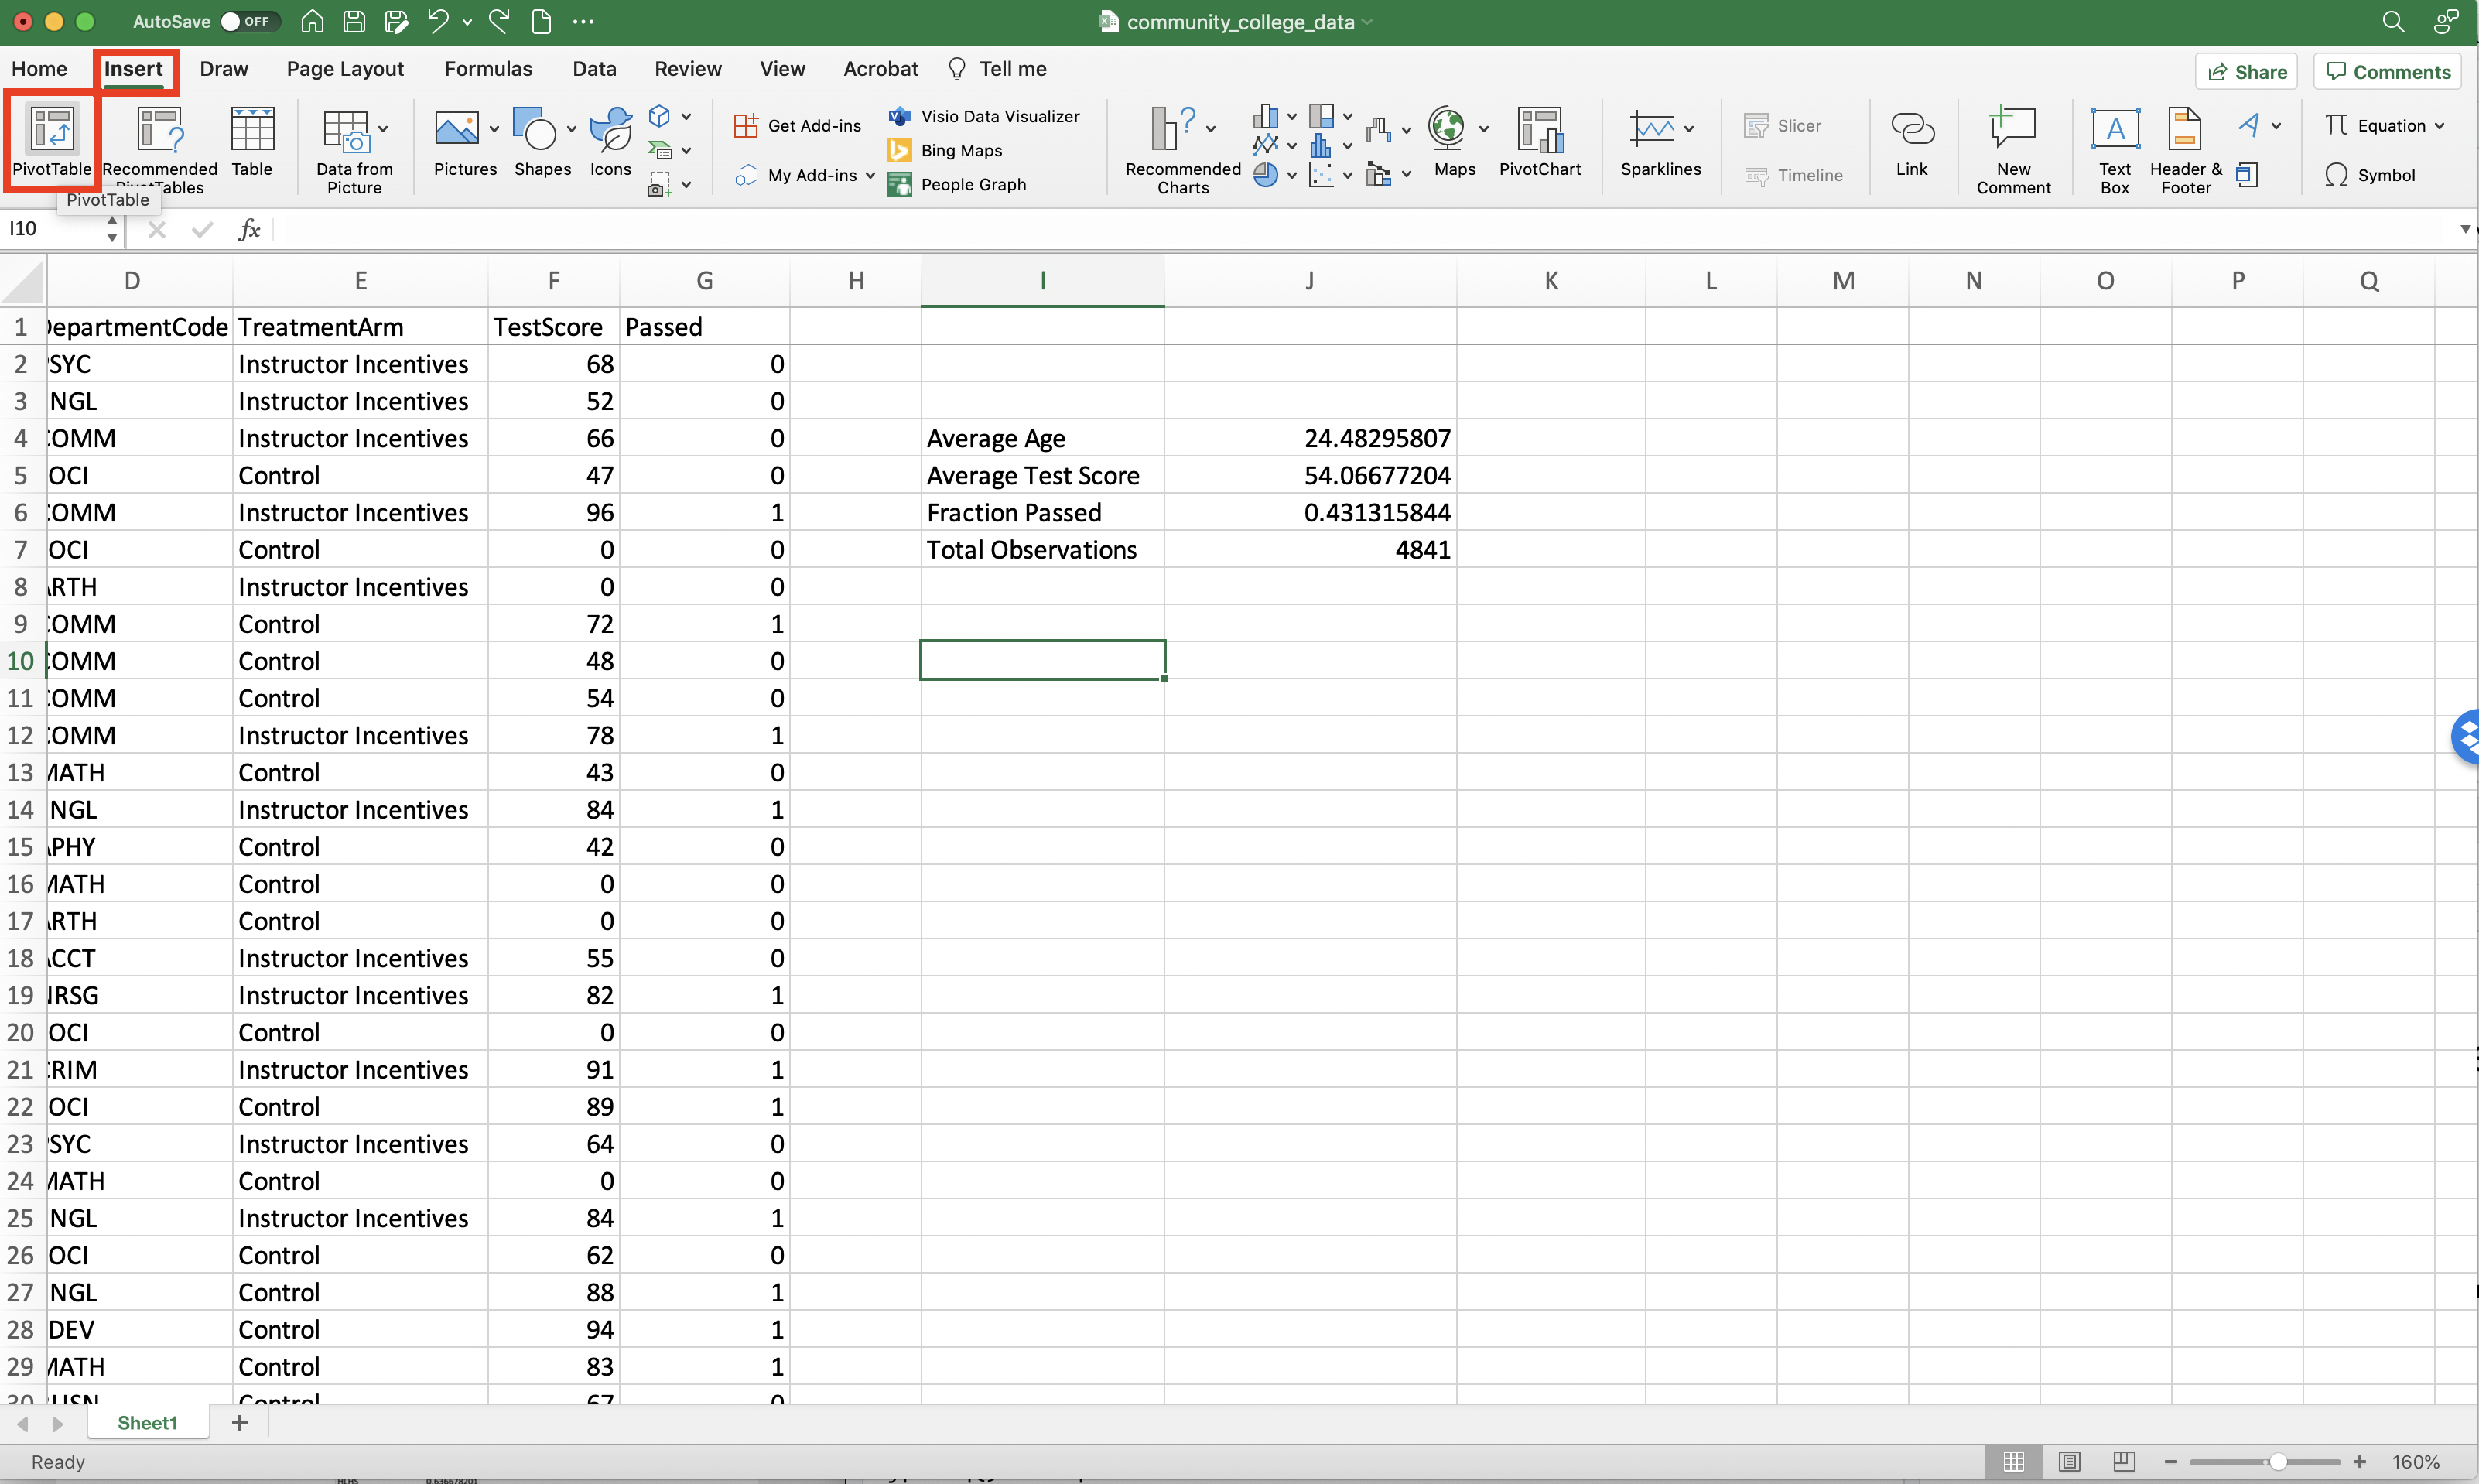
\includegraphics[width=1\linewidth]{images/01_pivot1} 

}

\caption{Inserting a Pivot Table}\label{fig:pivot1}
\end{figure}

Next, you need to select a table or range. You should select all of the variables that you want to be in your pivot table. In our case, we need to have both the department and whether an individual passed. To select a range, we can click on a column (for example D), hold down, and then drag to another column (for example G). Since we began at D and dragged to G, the variables \texttt{DepartmentCode}, \texttt{TreatmentArm}, \texttt{TestScore}, and \texttt{Passed} will all be variables that we can include in the pivot table.

\begin{figure}

{\centering 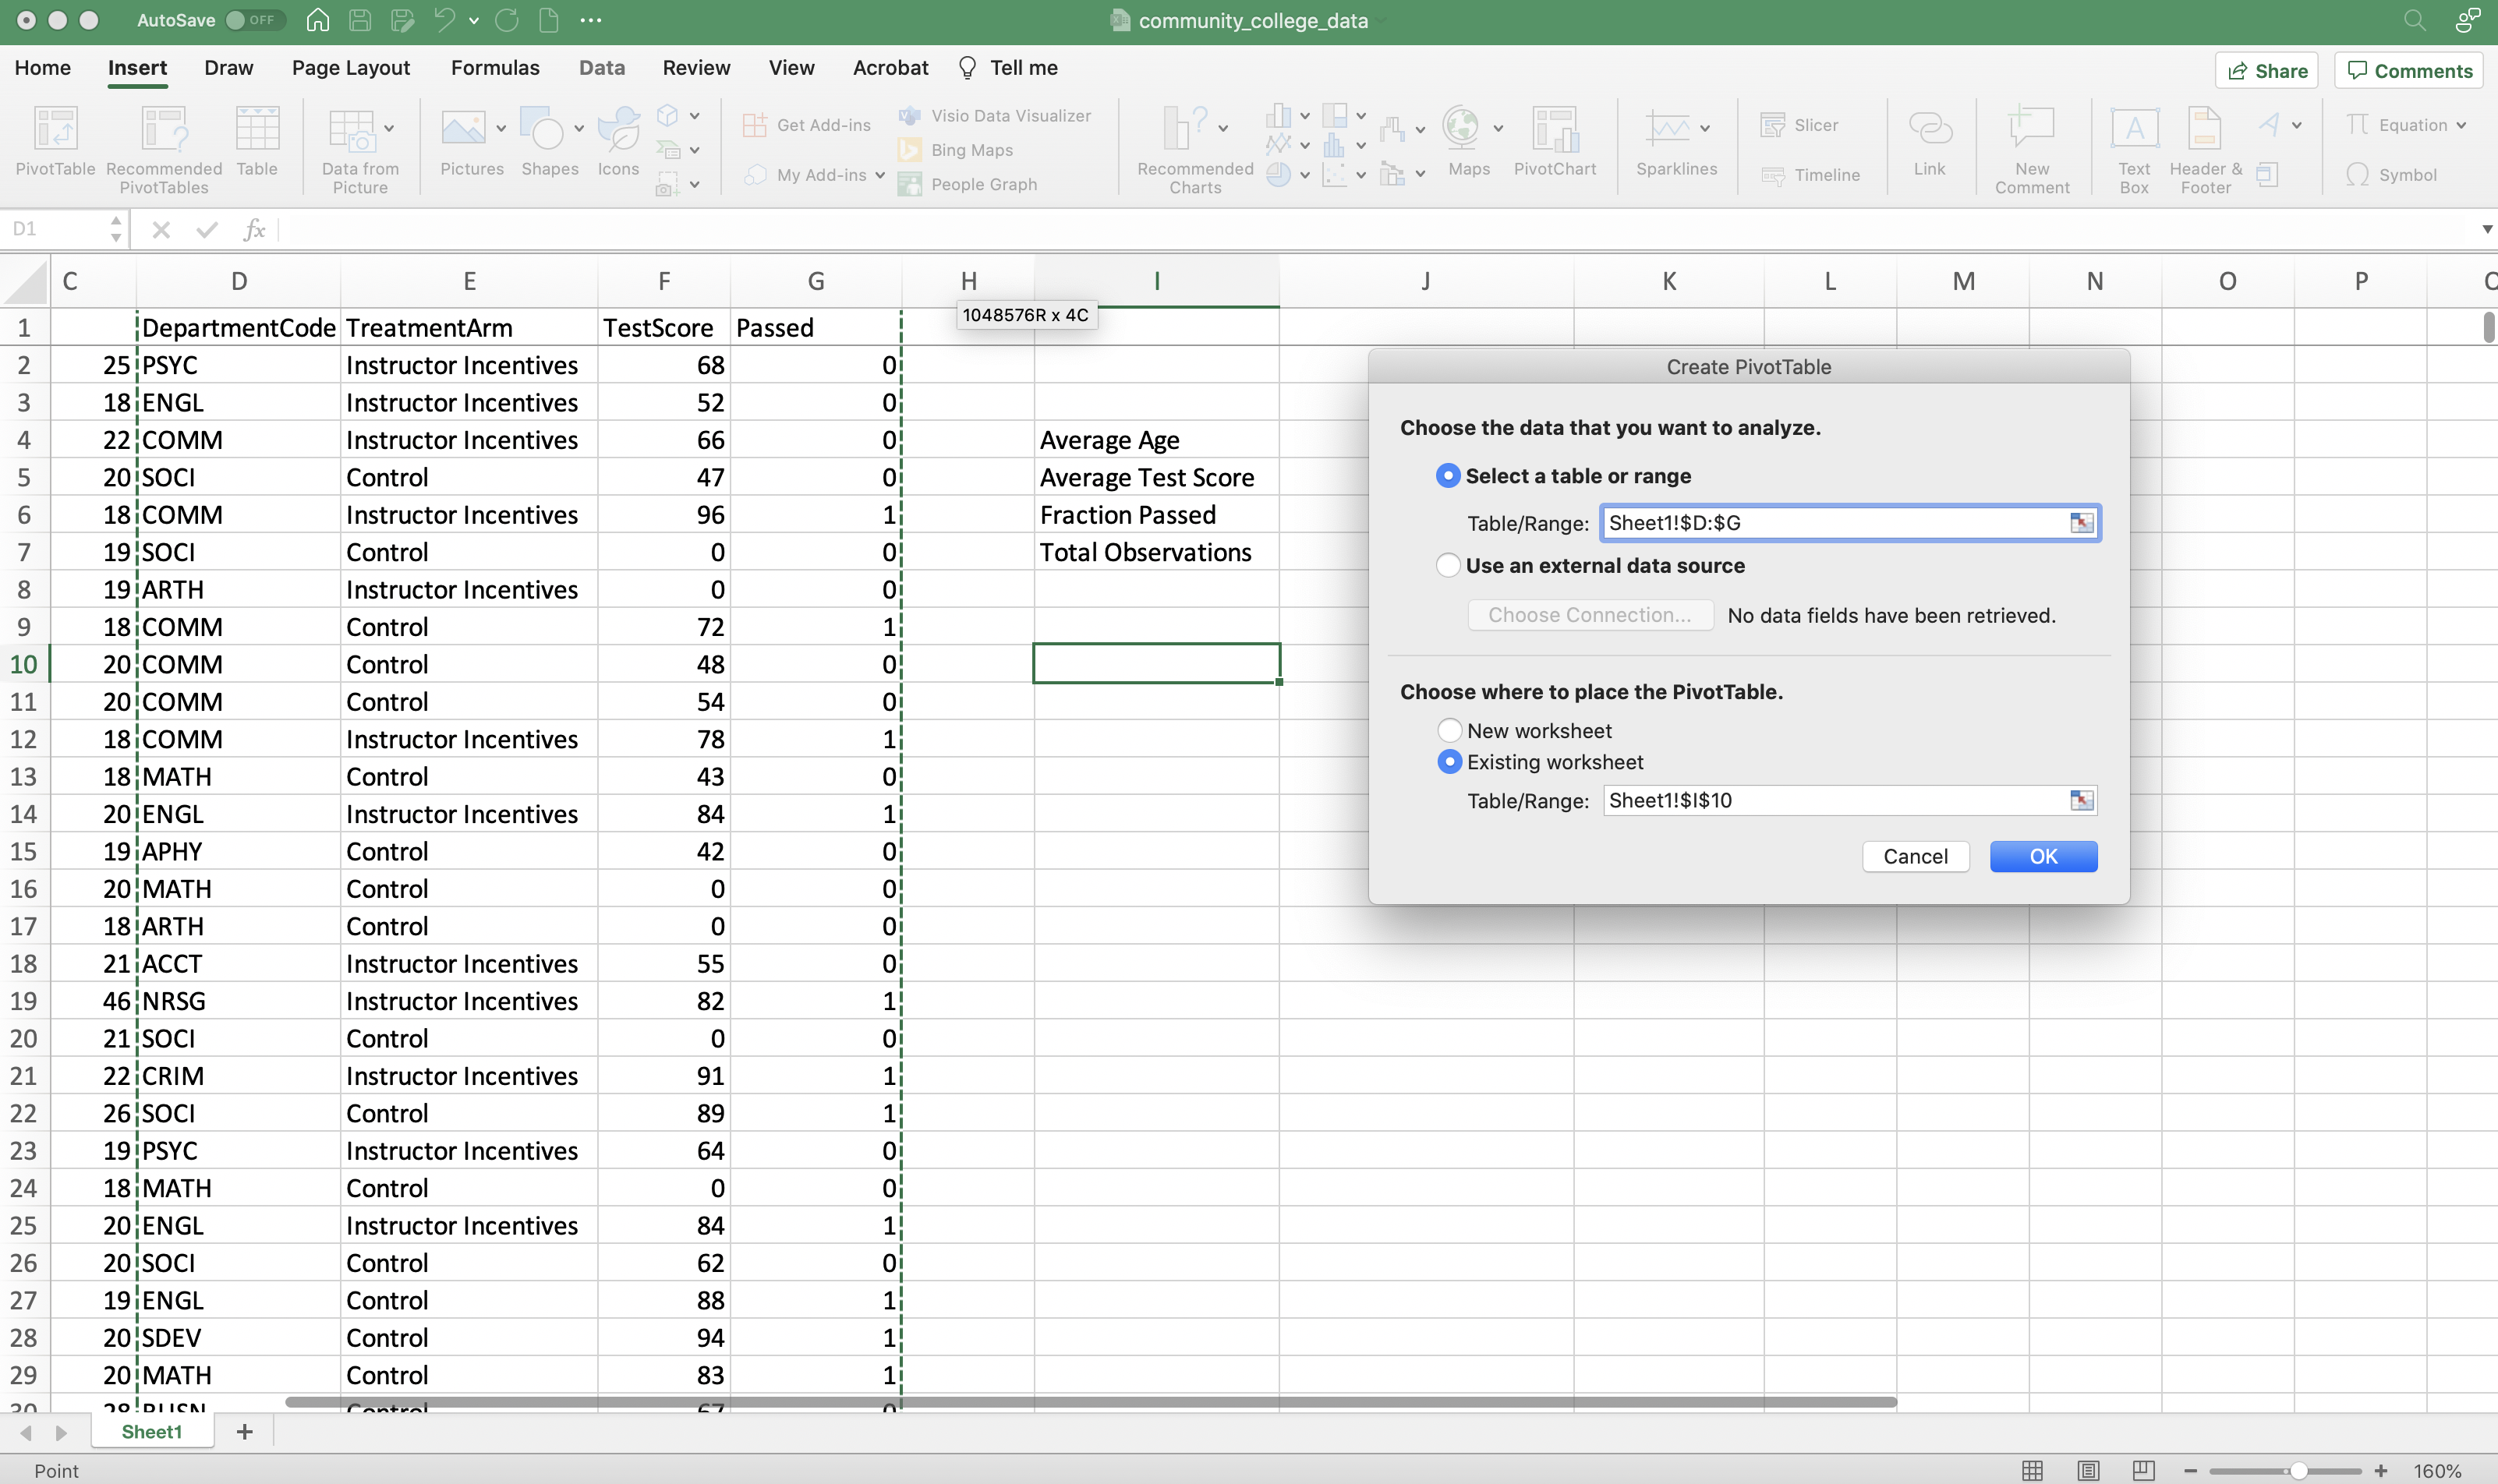
\includegraphics[width=1\linewidth]{images/01_pivot3} 

}

\caption{Selecting a Range for the Pivot Table}\label{fig:pivot3}
\end{figure}

You can also choose where you would like your pivot table to appear. By default, the table will be placed in whichever cell you clicked last (in my case this is cell \texttt{I10}). Therefore, before you insert a pivot table, you should click the cell where you would like it to appear.

As can be seen in Figure \ref{fig:pivot4}, Excel has drawn a blank Pivot table. On the right we can see the new panel ``PivotTable Fields'' which we will use to build our Pivot table

\begin{figure}

{\centering 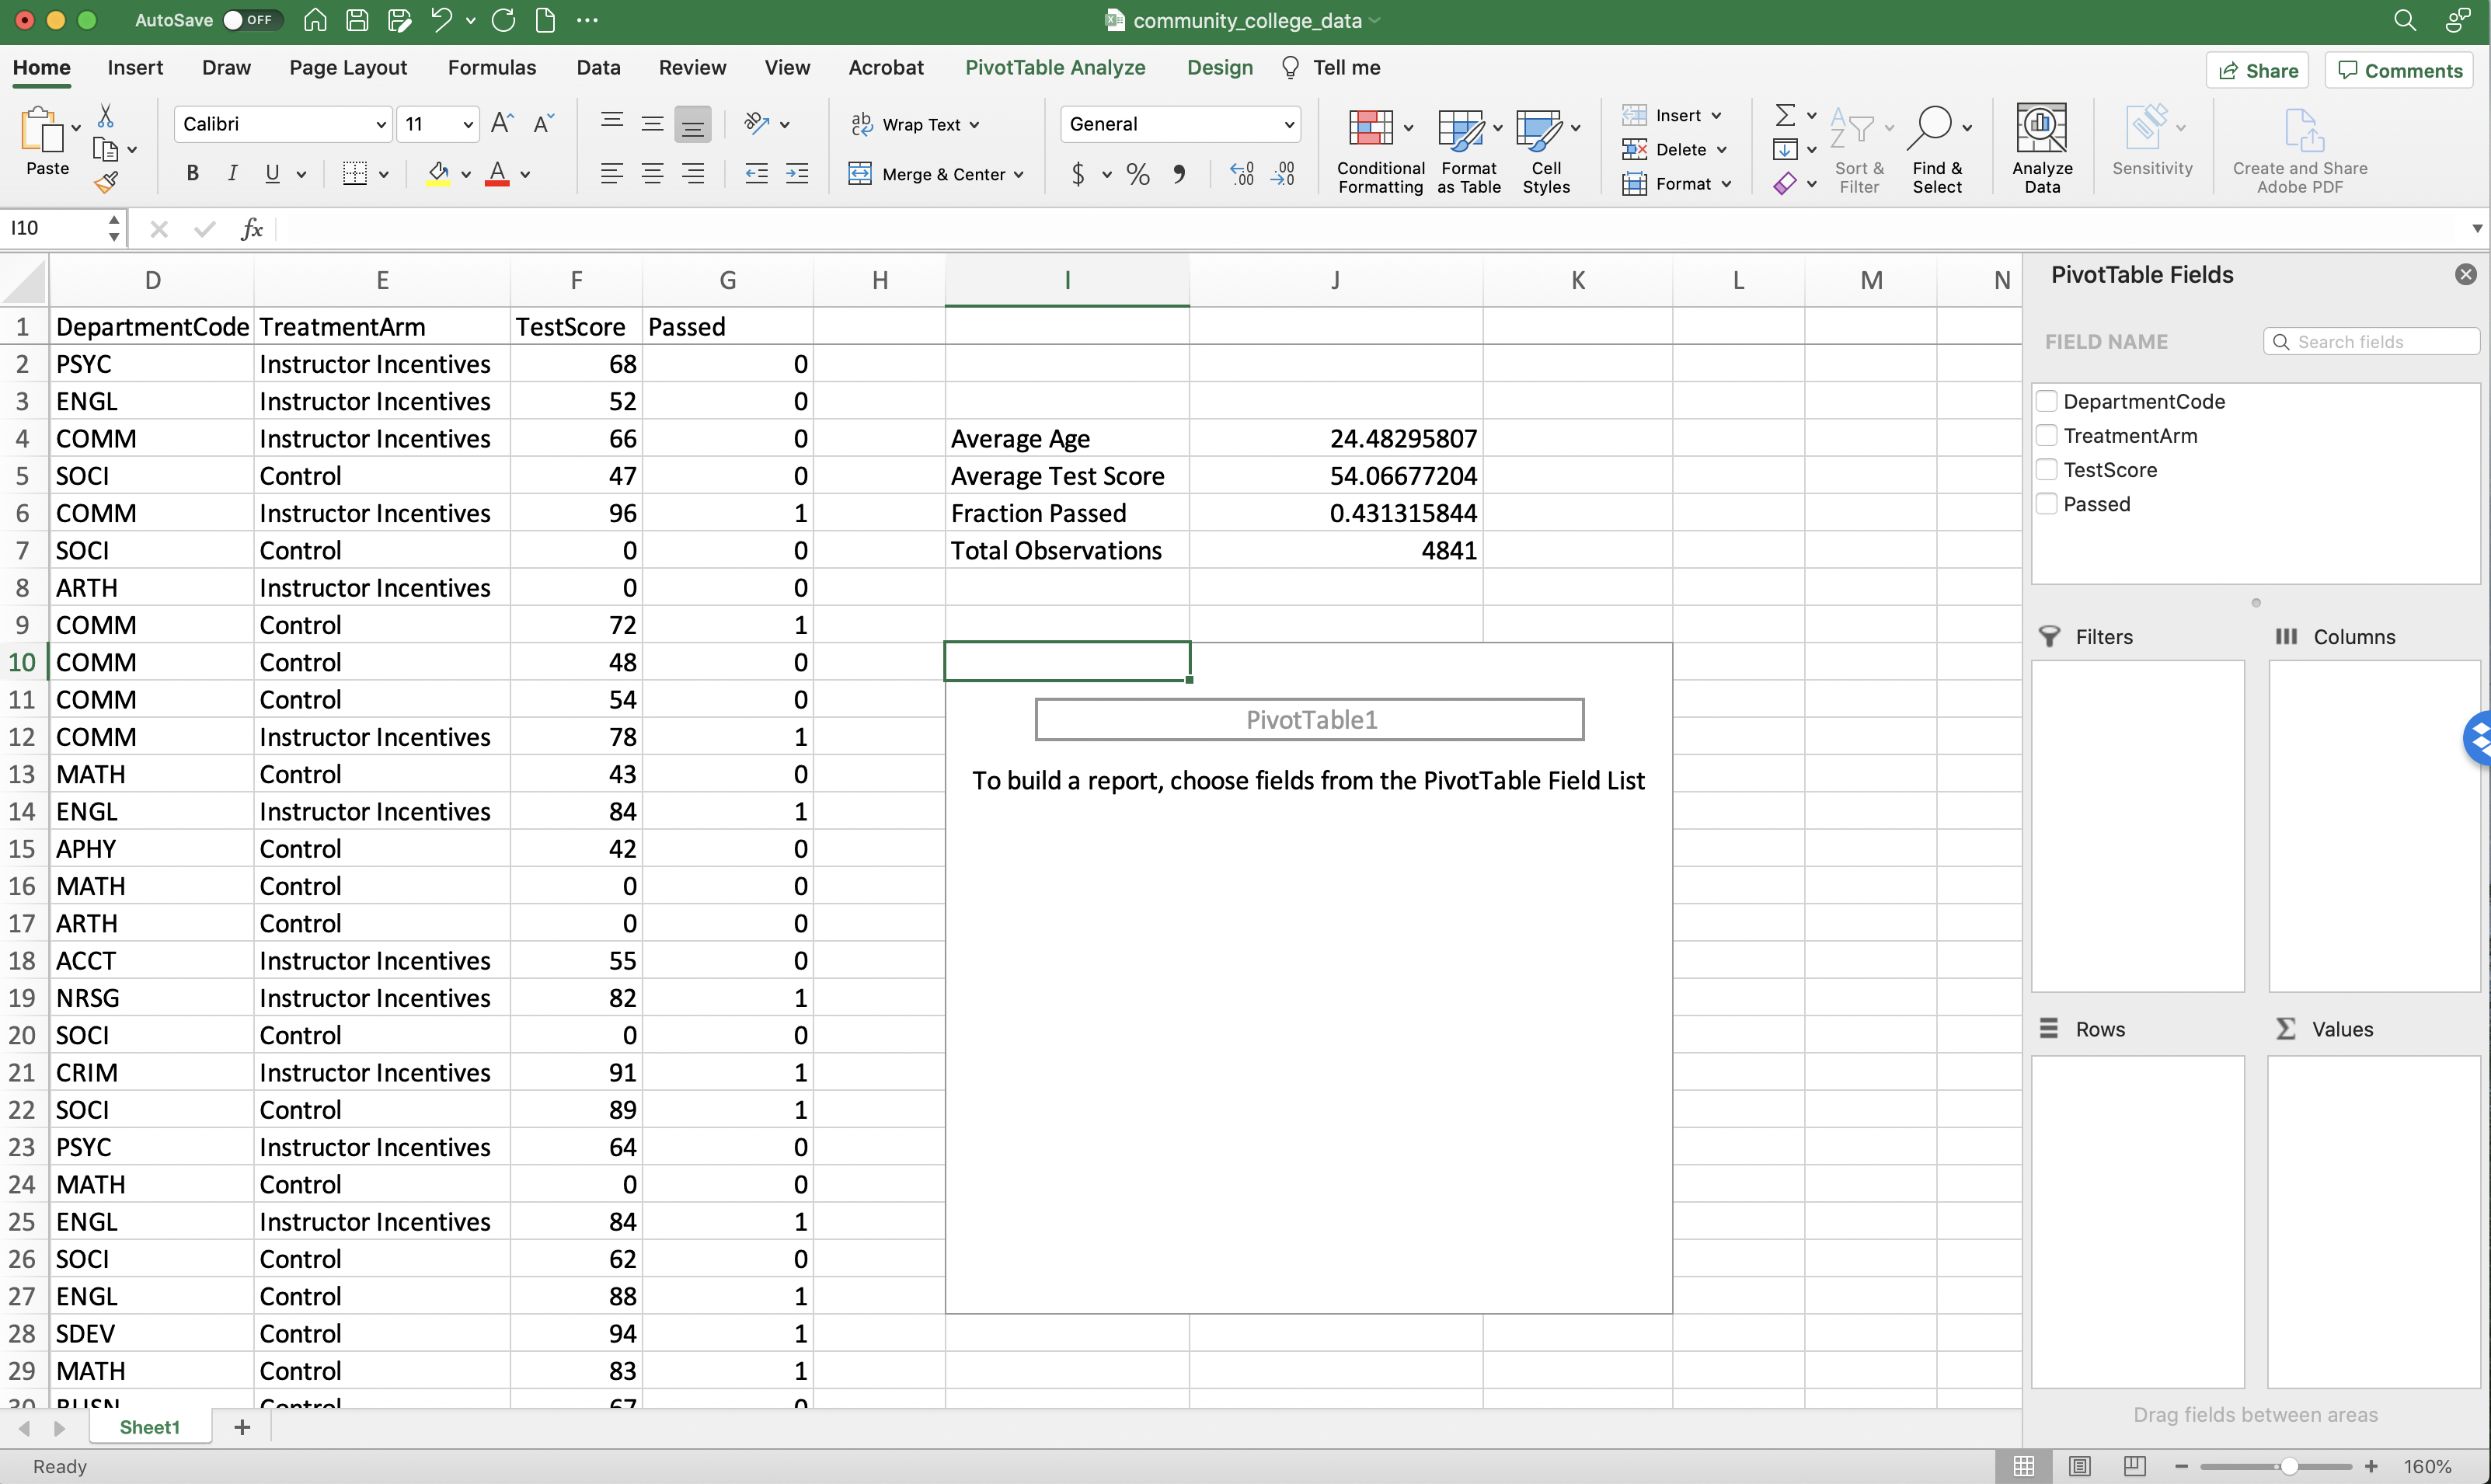
\includegraphics[width=1\linewidth]{images/01_pivot4} 

}

\caption{A Blank Pivot Table}\label{fig:pivot4}
\end{figure}

We want each row in our pivot table to be a Department Code. So click the box next to \texttt{DepartmentCode} to put it into the pivot table.

\begin{figure}

{\centering 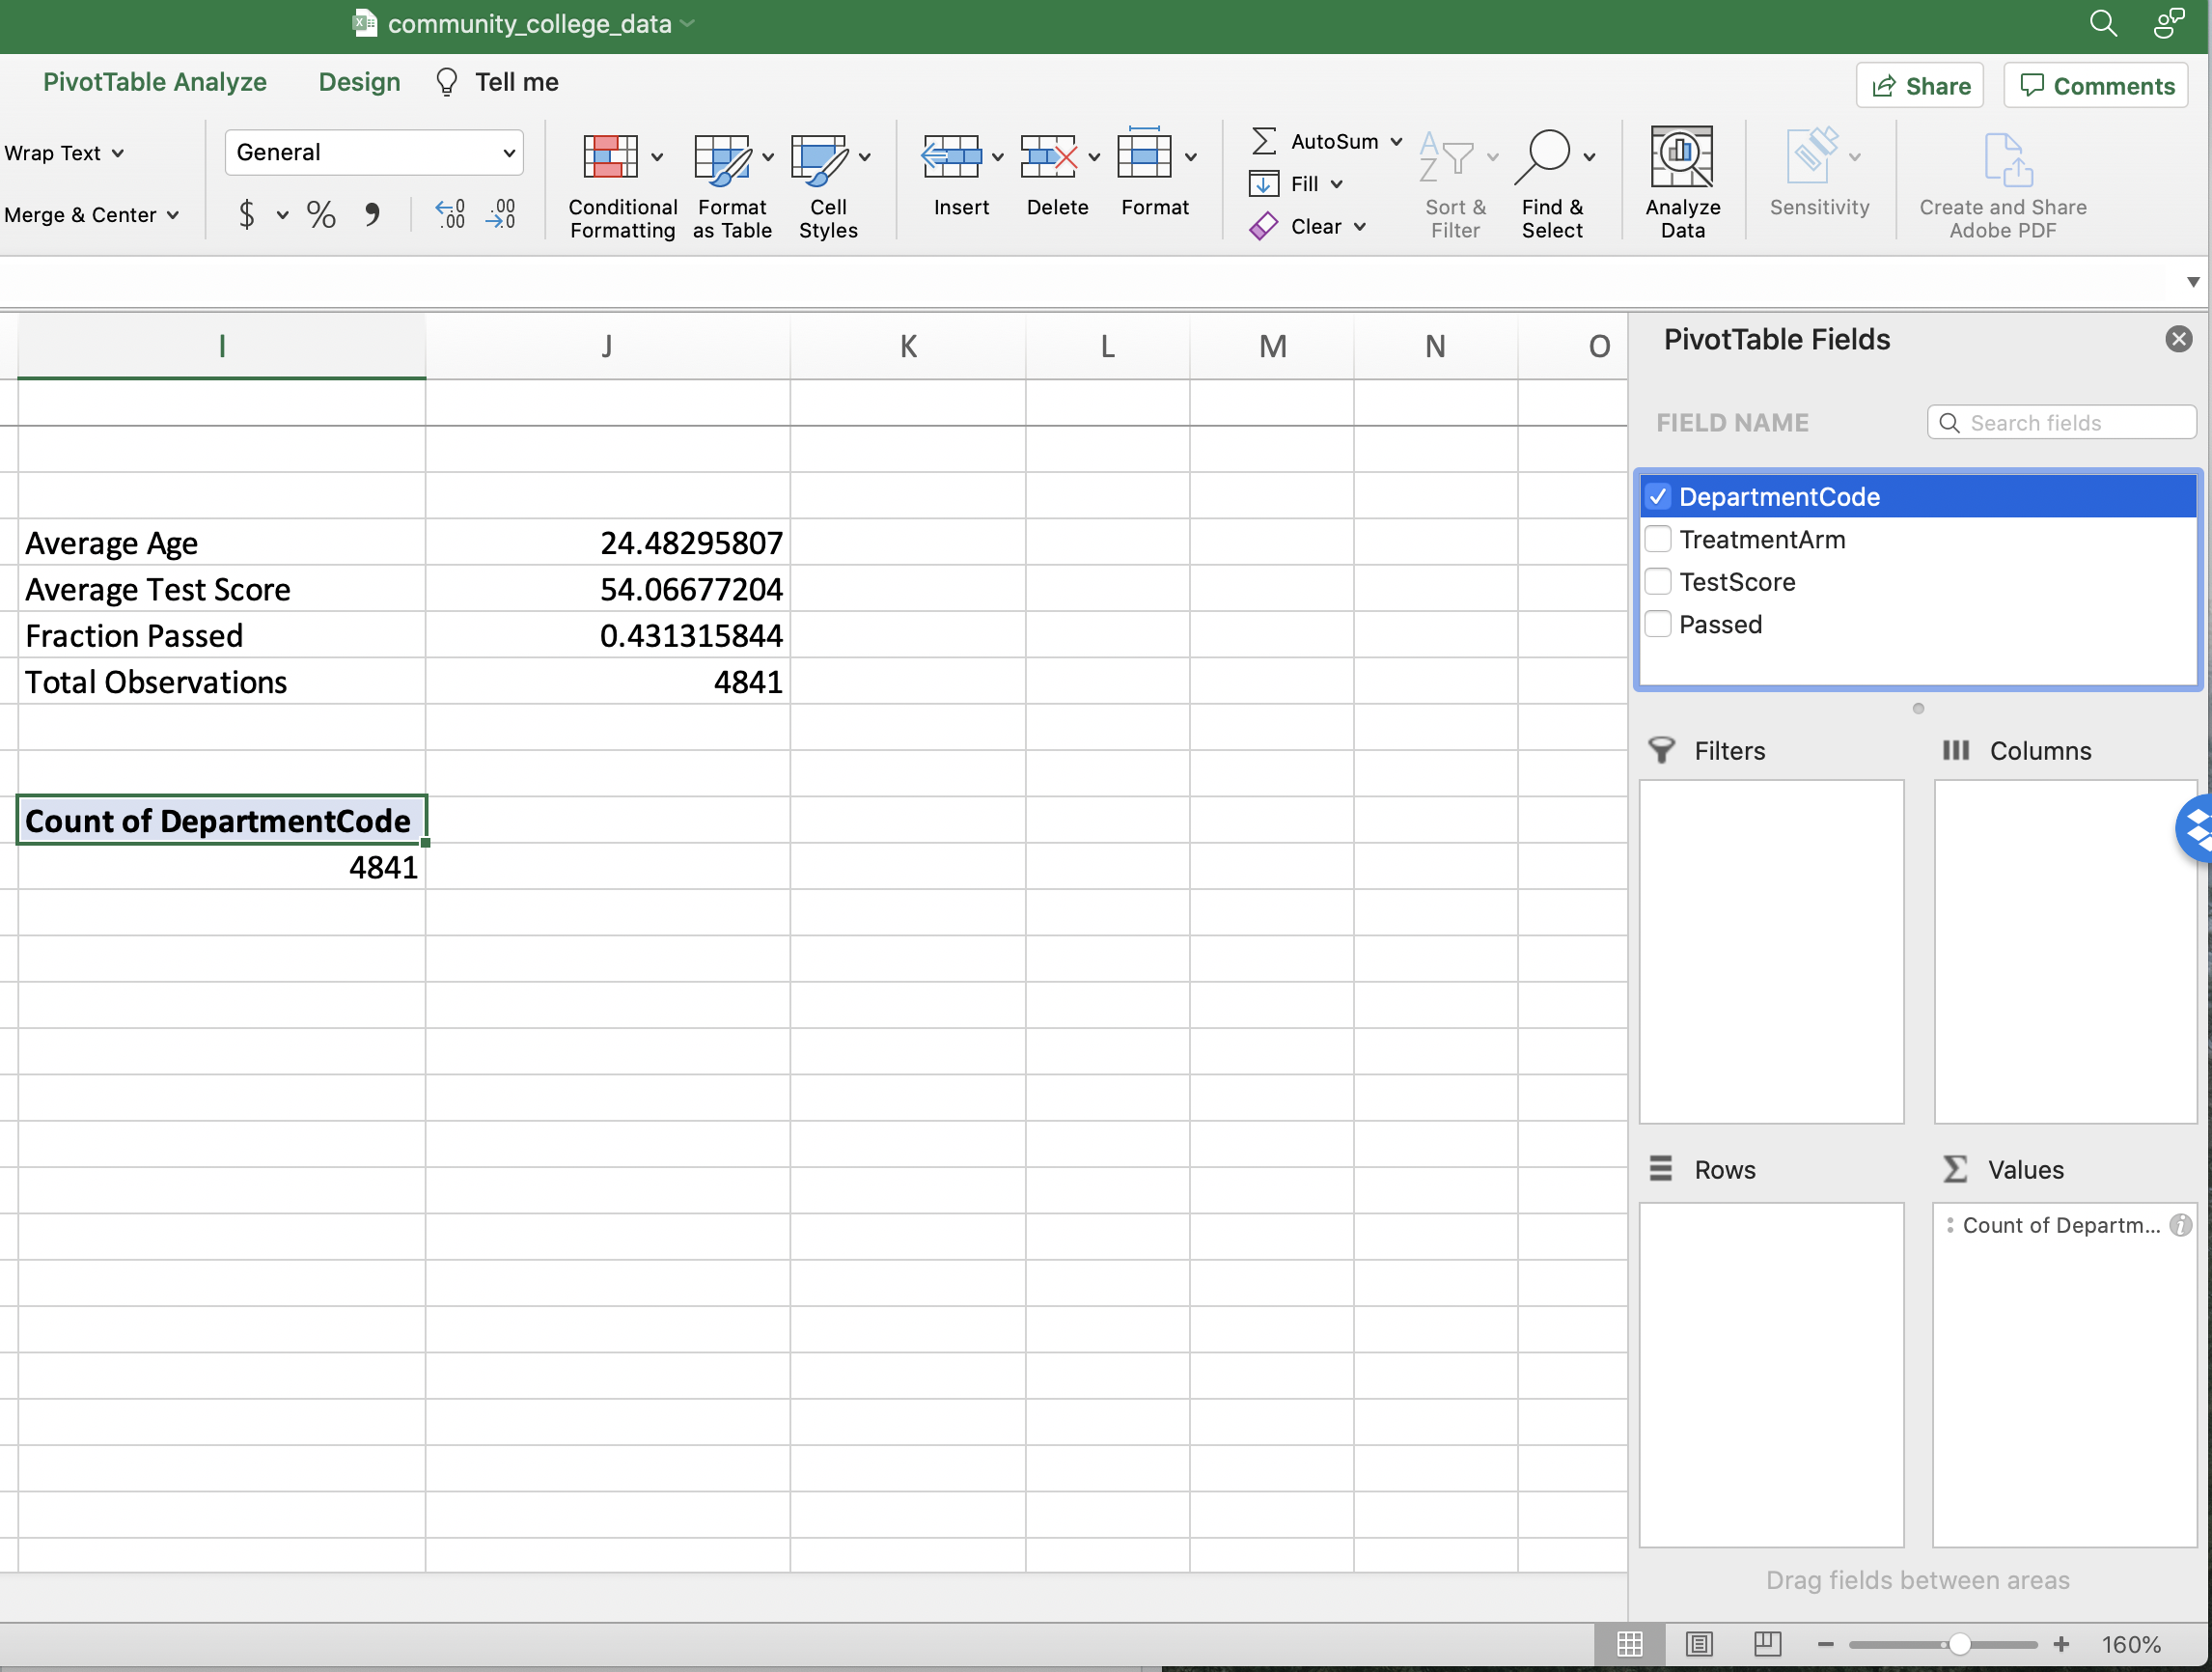
\includegraphics[width=1\linewidth]{images/01_pivot5} 

}

\caption{Adding DepartmentCode to the Pivot Table}\label{fig:pivot5}
\end{figure}

By default (see Figure \ref{fig:pivot5}), Excel has placed this variable into the Values panel, but we want it to be in the Rows panel. We can move variables between these windows by clicking and dragging. In this example we want to move \texttt{DepartmentCode} to the Rows panel.

\begin{figure}

{\centering 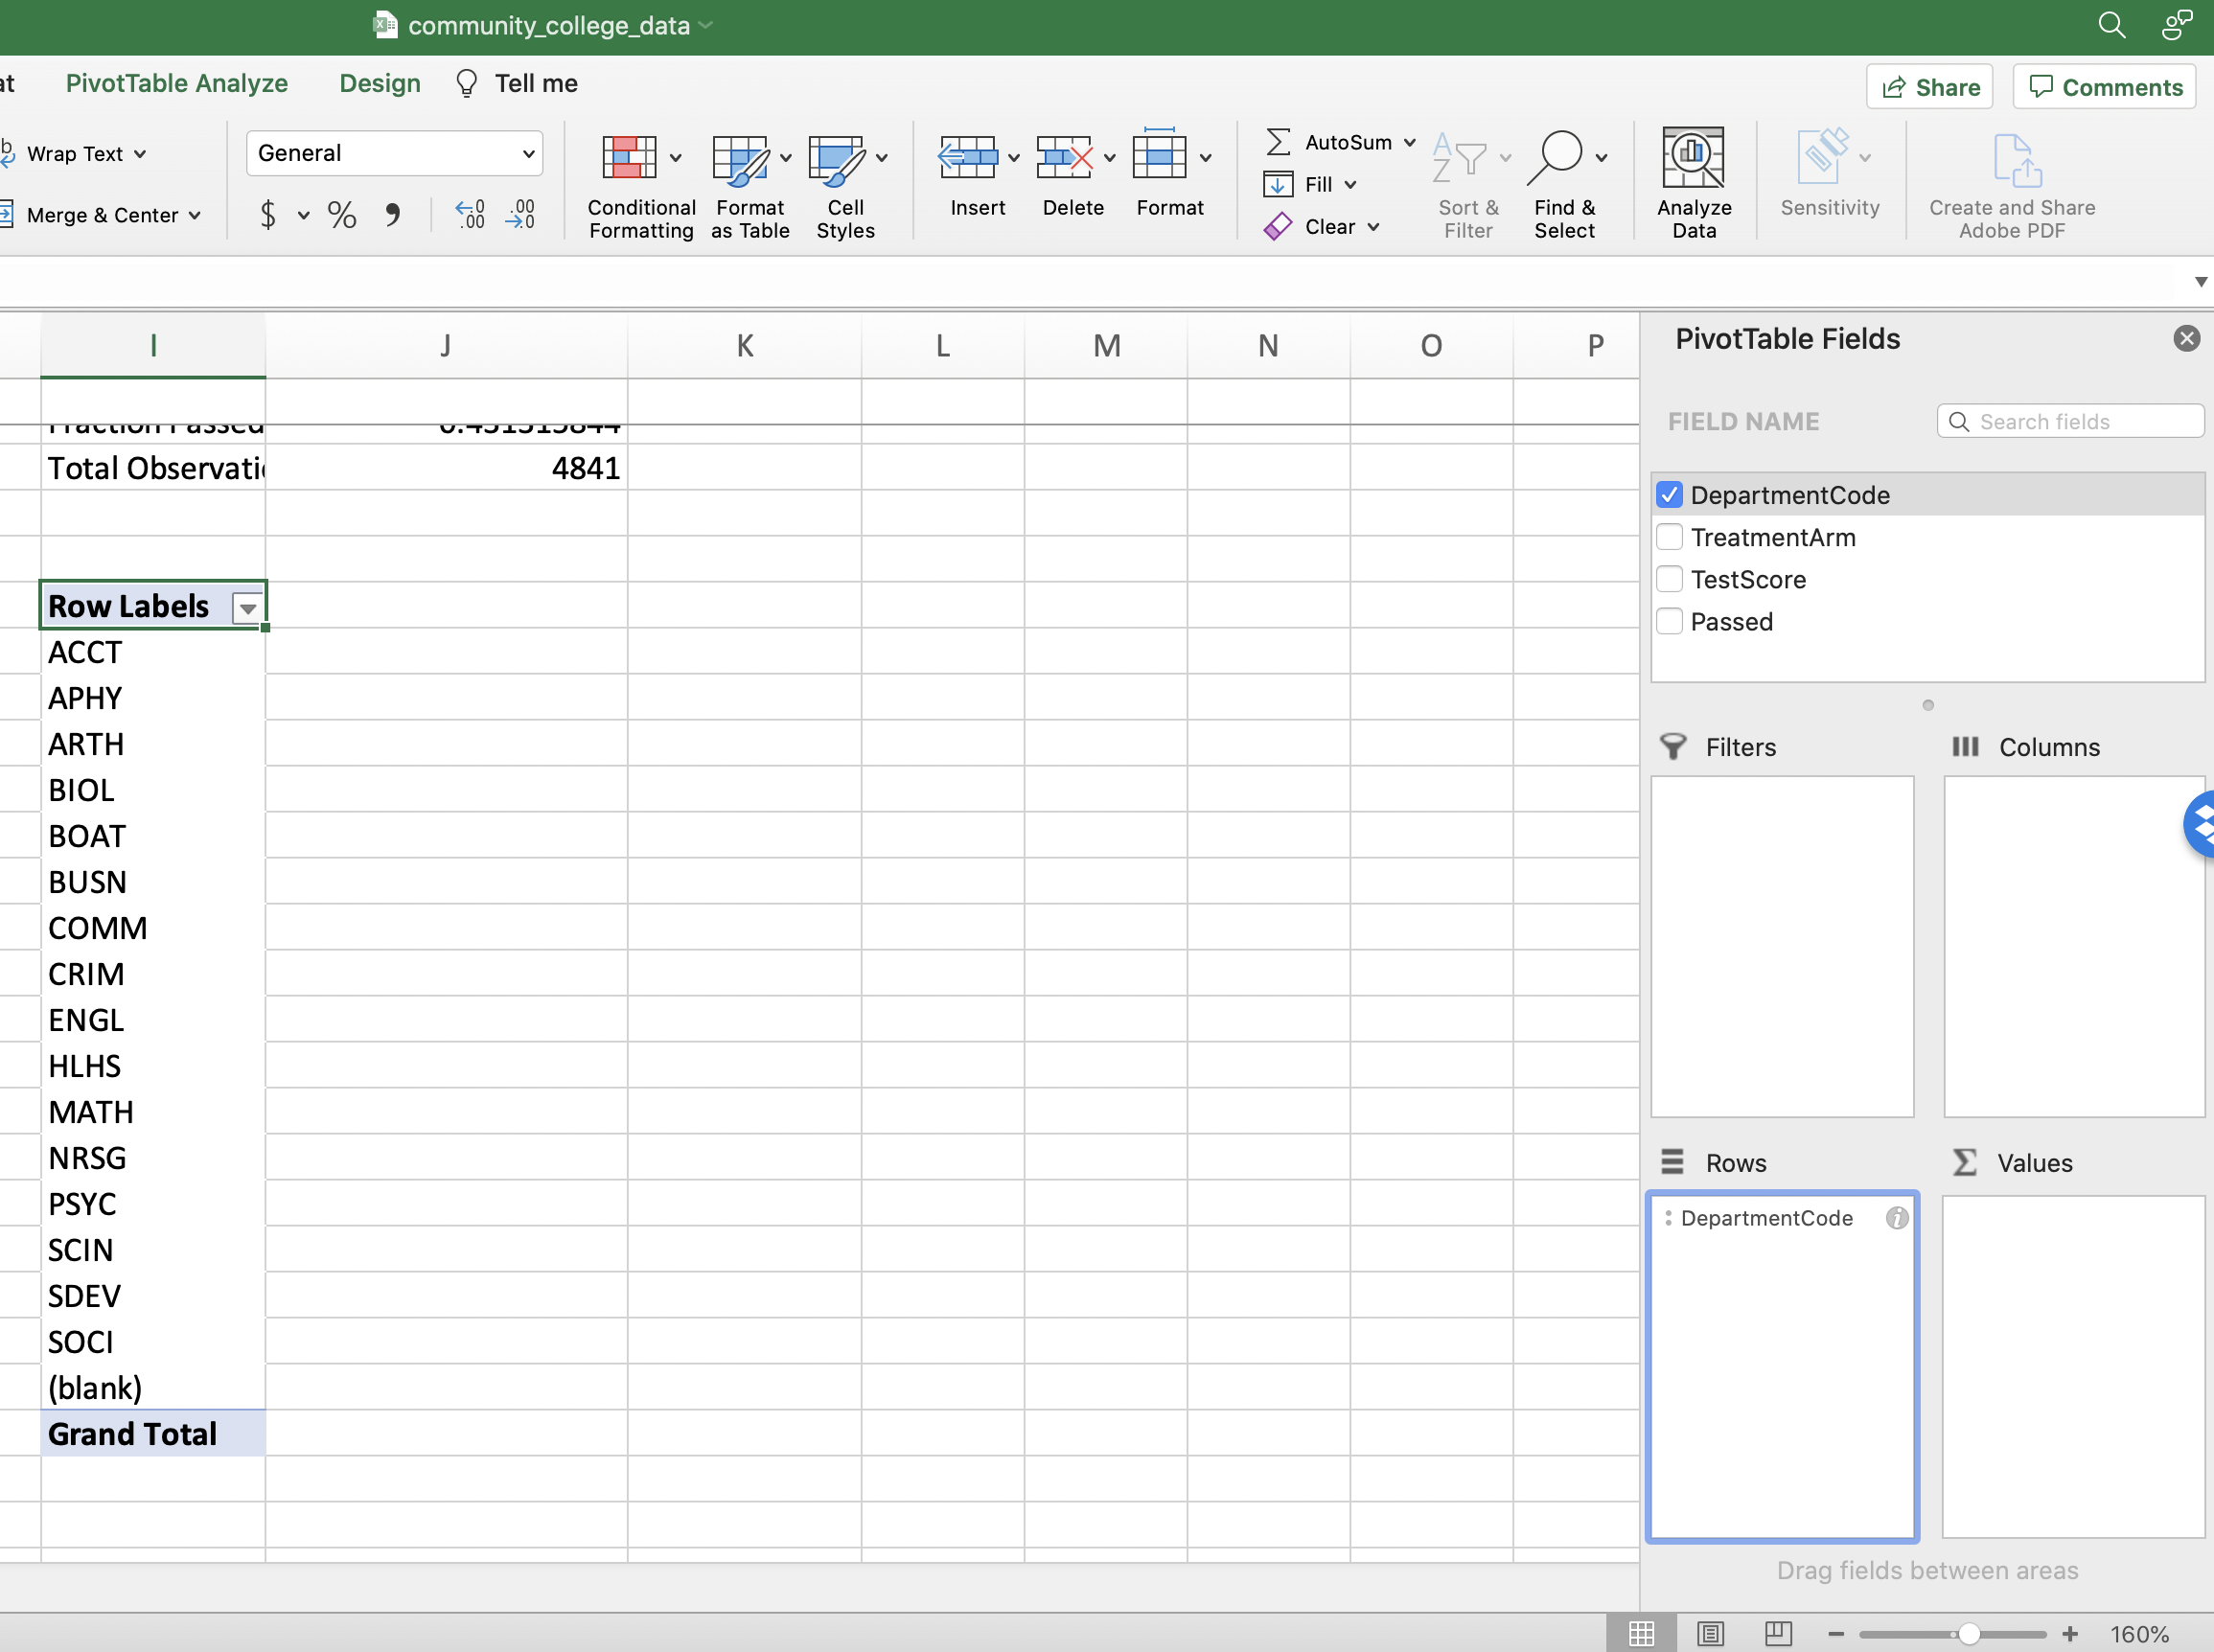
\includegraphics[width=1\linewidth]{images/01_pivot6} 

}

\caption{Adding DepartmentCode to the Pivot Table}\label{fig:pivot6}
\end{figure}

In the Values panel, we want pass rates. We will compute these pass rates from the variable ``Passed''

\begin{figure}

{\centering 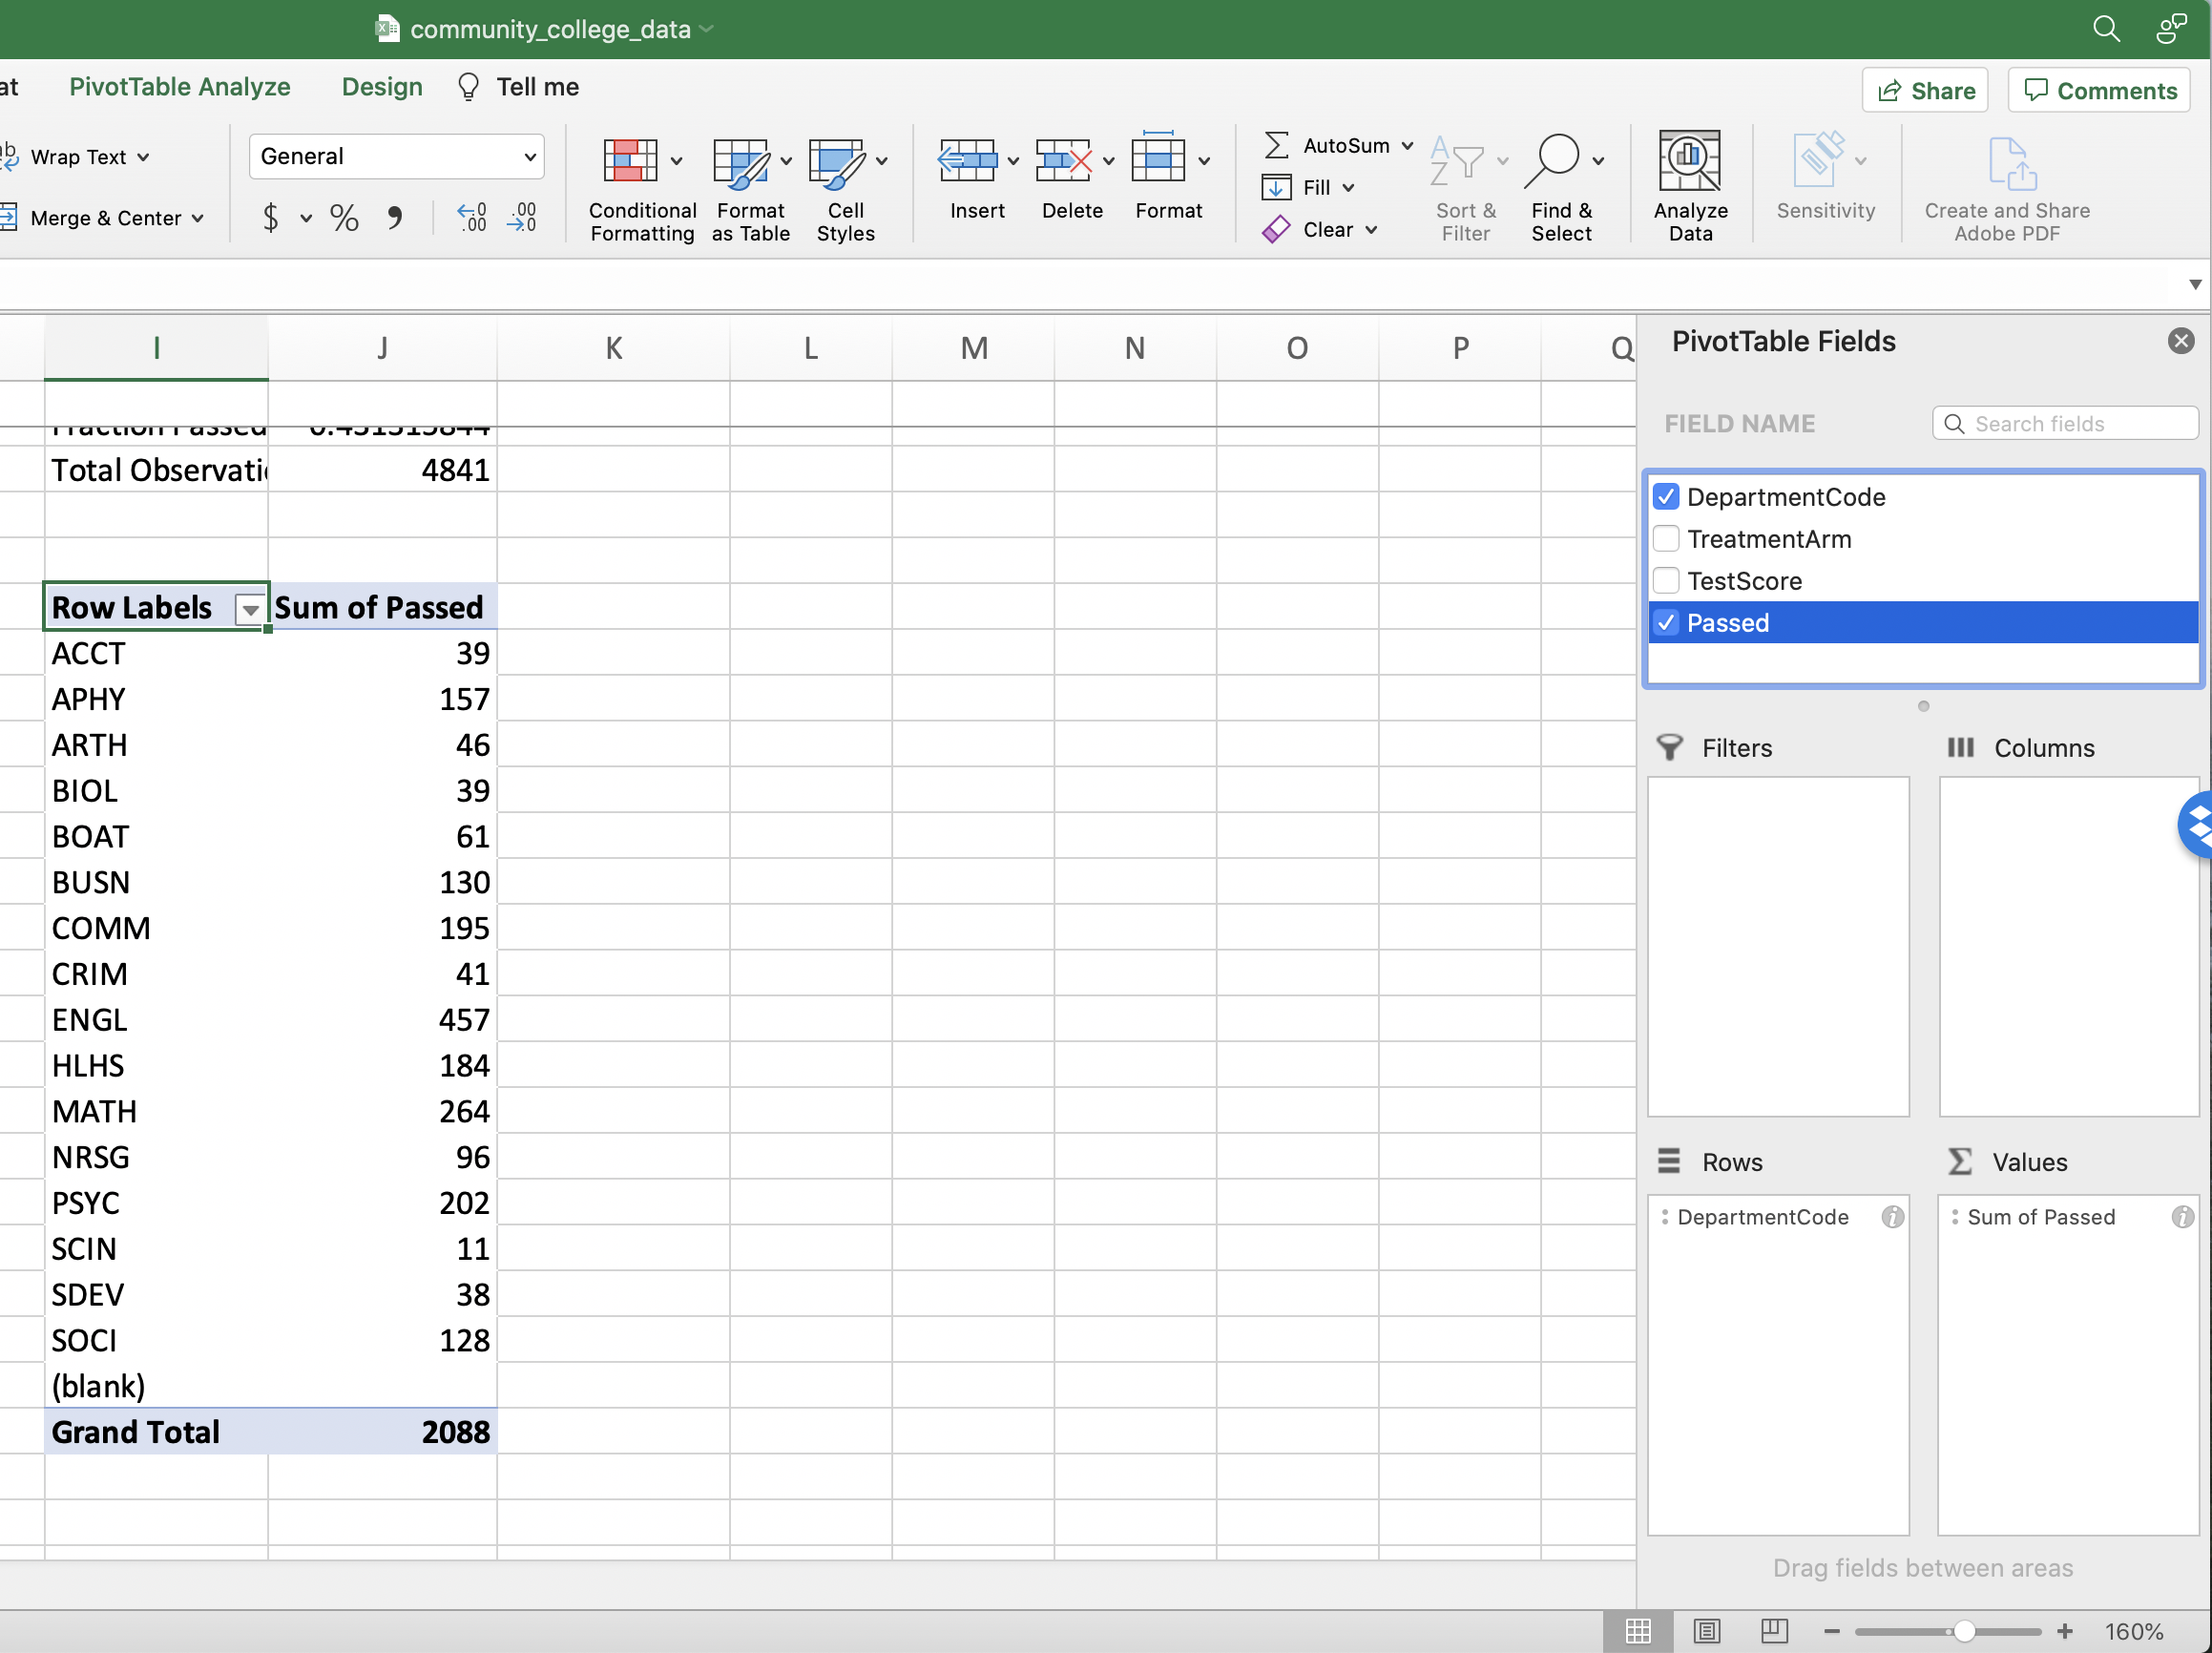
\includegraphics[width=1\linewidth]{images/01_pivot7} 

}

\caption{Adding Passed to the Pivot Table}\label{fig:pivot7}
\end{figure}

By default Excel is displaying the ``SUM'' by department (i.e.~number of individuals that passed, not the fraction that passed). To change the displayed statistic click the ``i'' next to the ``Values'' label and then select ``Average''.

\begin{figure}

{\centering 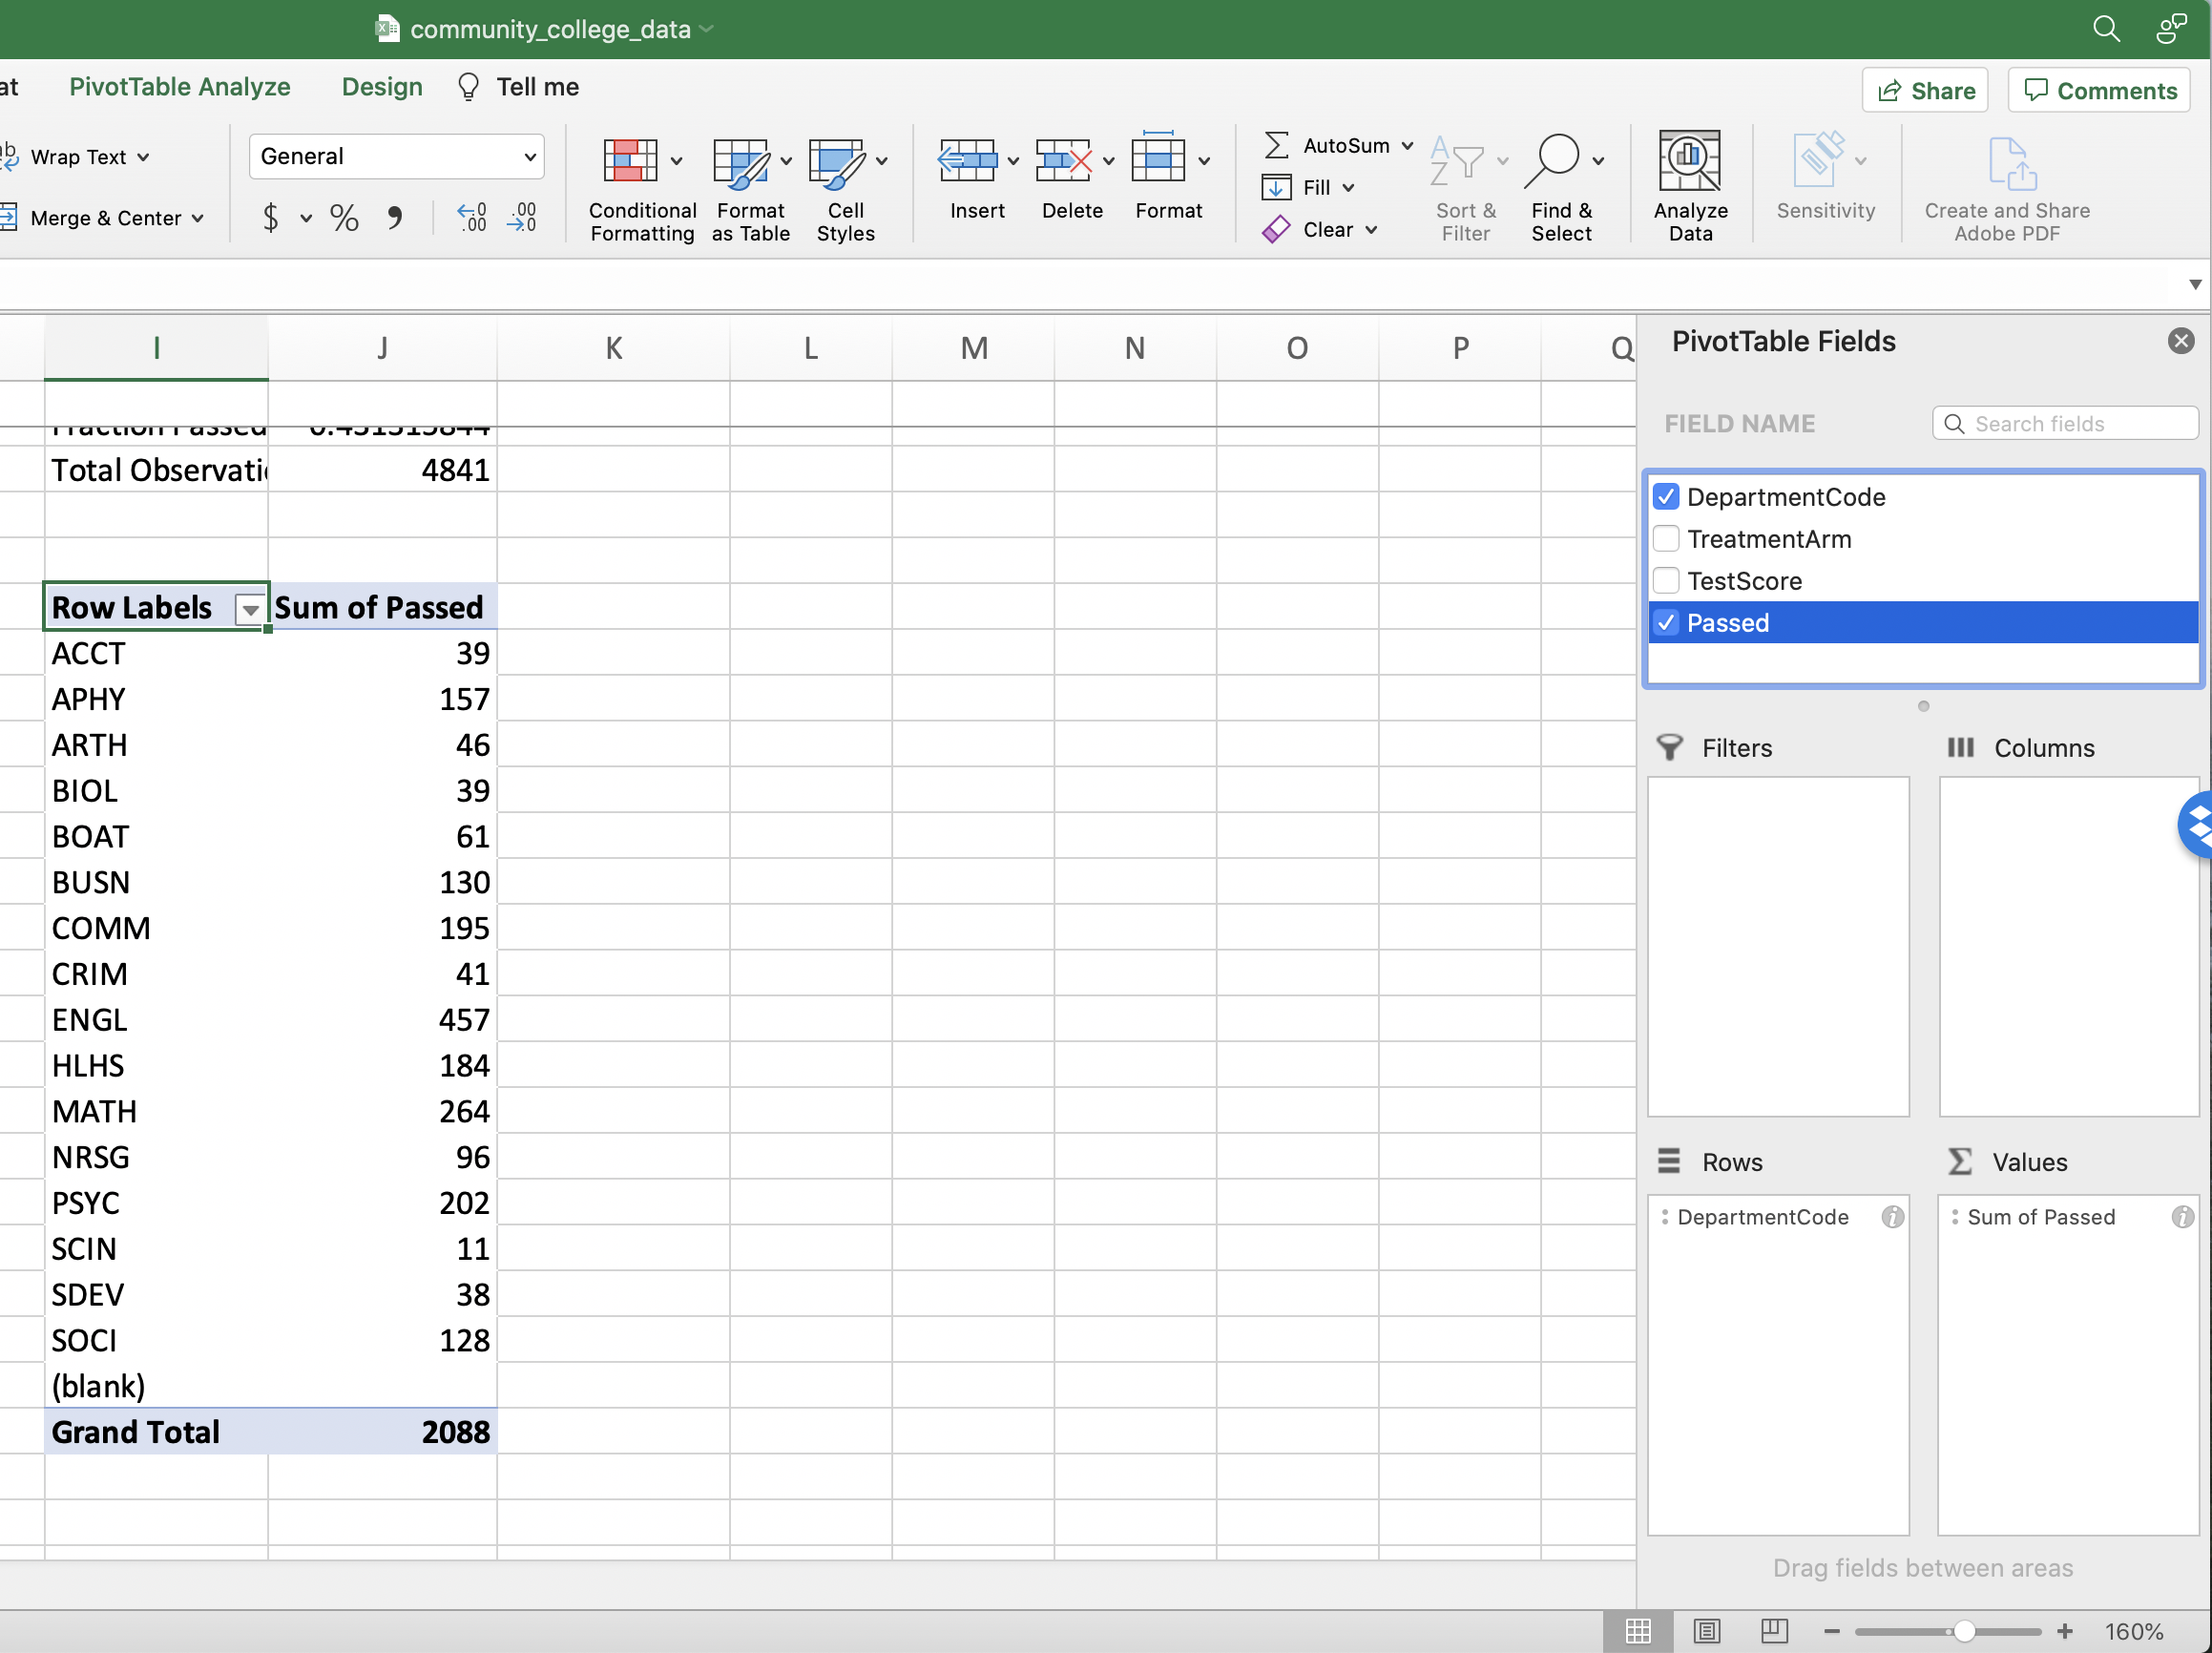
\includegraphics[width=1\linewidth]{images/01_pivot7} 

}

\caption{Average Pass Rates}\label{fig:pivot8}
\end{figure}

Now we've reached our goal! A table that shows average pass rates by department (Figure \ref{fig:pivotfinal}).

\hypertarget{balance-tables}{%
\section{Balance Tables}\label{balance-tables}}

The key aspect of a randomized control trial that allows us to infer causality is randomization. If randomization is successful, then individuals selected for the treatment should be similar (on average) to those selected for the control. Therefore, a key component of any analysis of experimental data is to show that the treatment and control are similar based on observable characteristics.

To understand how a balance test might fail, let's imagine researchers are testing whether a given drug reduces cholesterol. The experimenters receive a list of 200 participants for the trial and decide the first 100 names on the list will receive the treatment and the second 100 will receive the placebo. What they fail to realize is that the list of applicants is sorted from youngest to oldest. Therefore, only the youngest participants receive the treatment. But younger applicants, on average, probably have lower cholesterol to begin with, so differences between treatment and control may be due to age, not due to the treatment.

If we perform a balance test (i.e.~calculate average age by treatment and control) we would immediately detect our error. Now, no ``real'' experiment would ever be run in such a way. To do so would be ignoring standard protocol for well-run experiments! Still, it is important to understand whether there are differences between treated and control units before proceeding with the main analysis.Finding persistent differences with respect to observables could be evidence that randomization somehow failed. In our empirical application, we have information on the age of the student, so let's see if age varies between the treatment and control.

We want to retrieve the average age by Treatment Arm. To do so we can use a pivot table! The \textbf{Rows} will be the Treatment Arm, while the \textbf{Values} will be age. We can follow the exact same steps as in Section @ref(heading.pivottable)

\hypertarget{intergenerational-mobility-and-higher-education-stata}{%
\chapter{Intergenerational Mobility and Higher Education (Stata)}\label{intergenerational-mobility-and-higher-education-stata}}

\hypertarget{intergenerational-mobility}{%
\section{Intergenerational Mobility}\label{intergenerational-mobility}}

In this section, we will be discussing the relationship between \textbf{intergenerational mobility} and the higher education system in the United Stata. Before we start exploring this relationship, we first need to understand the concept of intergenerational mobility. This concept asks a simple question: if you are born from low-income parents, what is the chance you move up the income distribution?

Generally, we think of societies with high rates of intergenerational mobility as more equal. If a society has high rates of intergenerational mobility, then that means individuals from low-income backgrounds have opportunities to move up the income distribution. One common path to upward mobility is the higher education system.

However, there are a few reasons why the higher education system may or may not lead to higher rates of intergenerational mobility. First, some colleges may not be particularly effective in increasing incomes. For example, for-profit colleges are often criticized as costly and low quality (See \href{https://www.nytimes.com/2020/06/17/business/coronavirus-for-profit-colleges.html}{NYT Article}). If a college accepts a large fraction of students from low-income backgrounds, it may still not promote intergenerational mobility if its students don't actually benefit from attending. Second, individuals from lower-income backgrounds may have lower access to the higher education system. Rising cost of college may be making this worse over time.

So how do we go about studying this question? We are going to use a dataset made publicly available by the researchers at \textbf{Opportunity Insights}. This data has made a big splash, both in academia and in policy circles.Figure \ref{fig:oi} shows a headline from an Upshot article about the dataset. In this article, the authors discuss how this dataset has led us to new insights about how access varies dramatically at some schools. The headline reads, ``Some Colleges Have More Students From the Top 1 Percent Than the Bottom 60. Find Yours''. If a school has more students from the top 1 percent than the bottom 60, then it probably does not promote intergenerational mobility. Most of the students are already from relatively well-off backgrounds. This is our first hint that colleges may vary dramatically in the extent that they promote intergenerational mobility.

\begin{figure}

{\centering 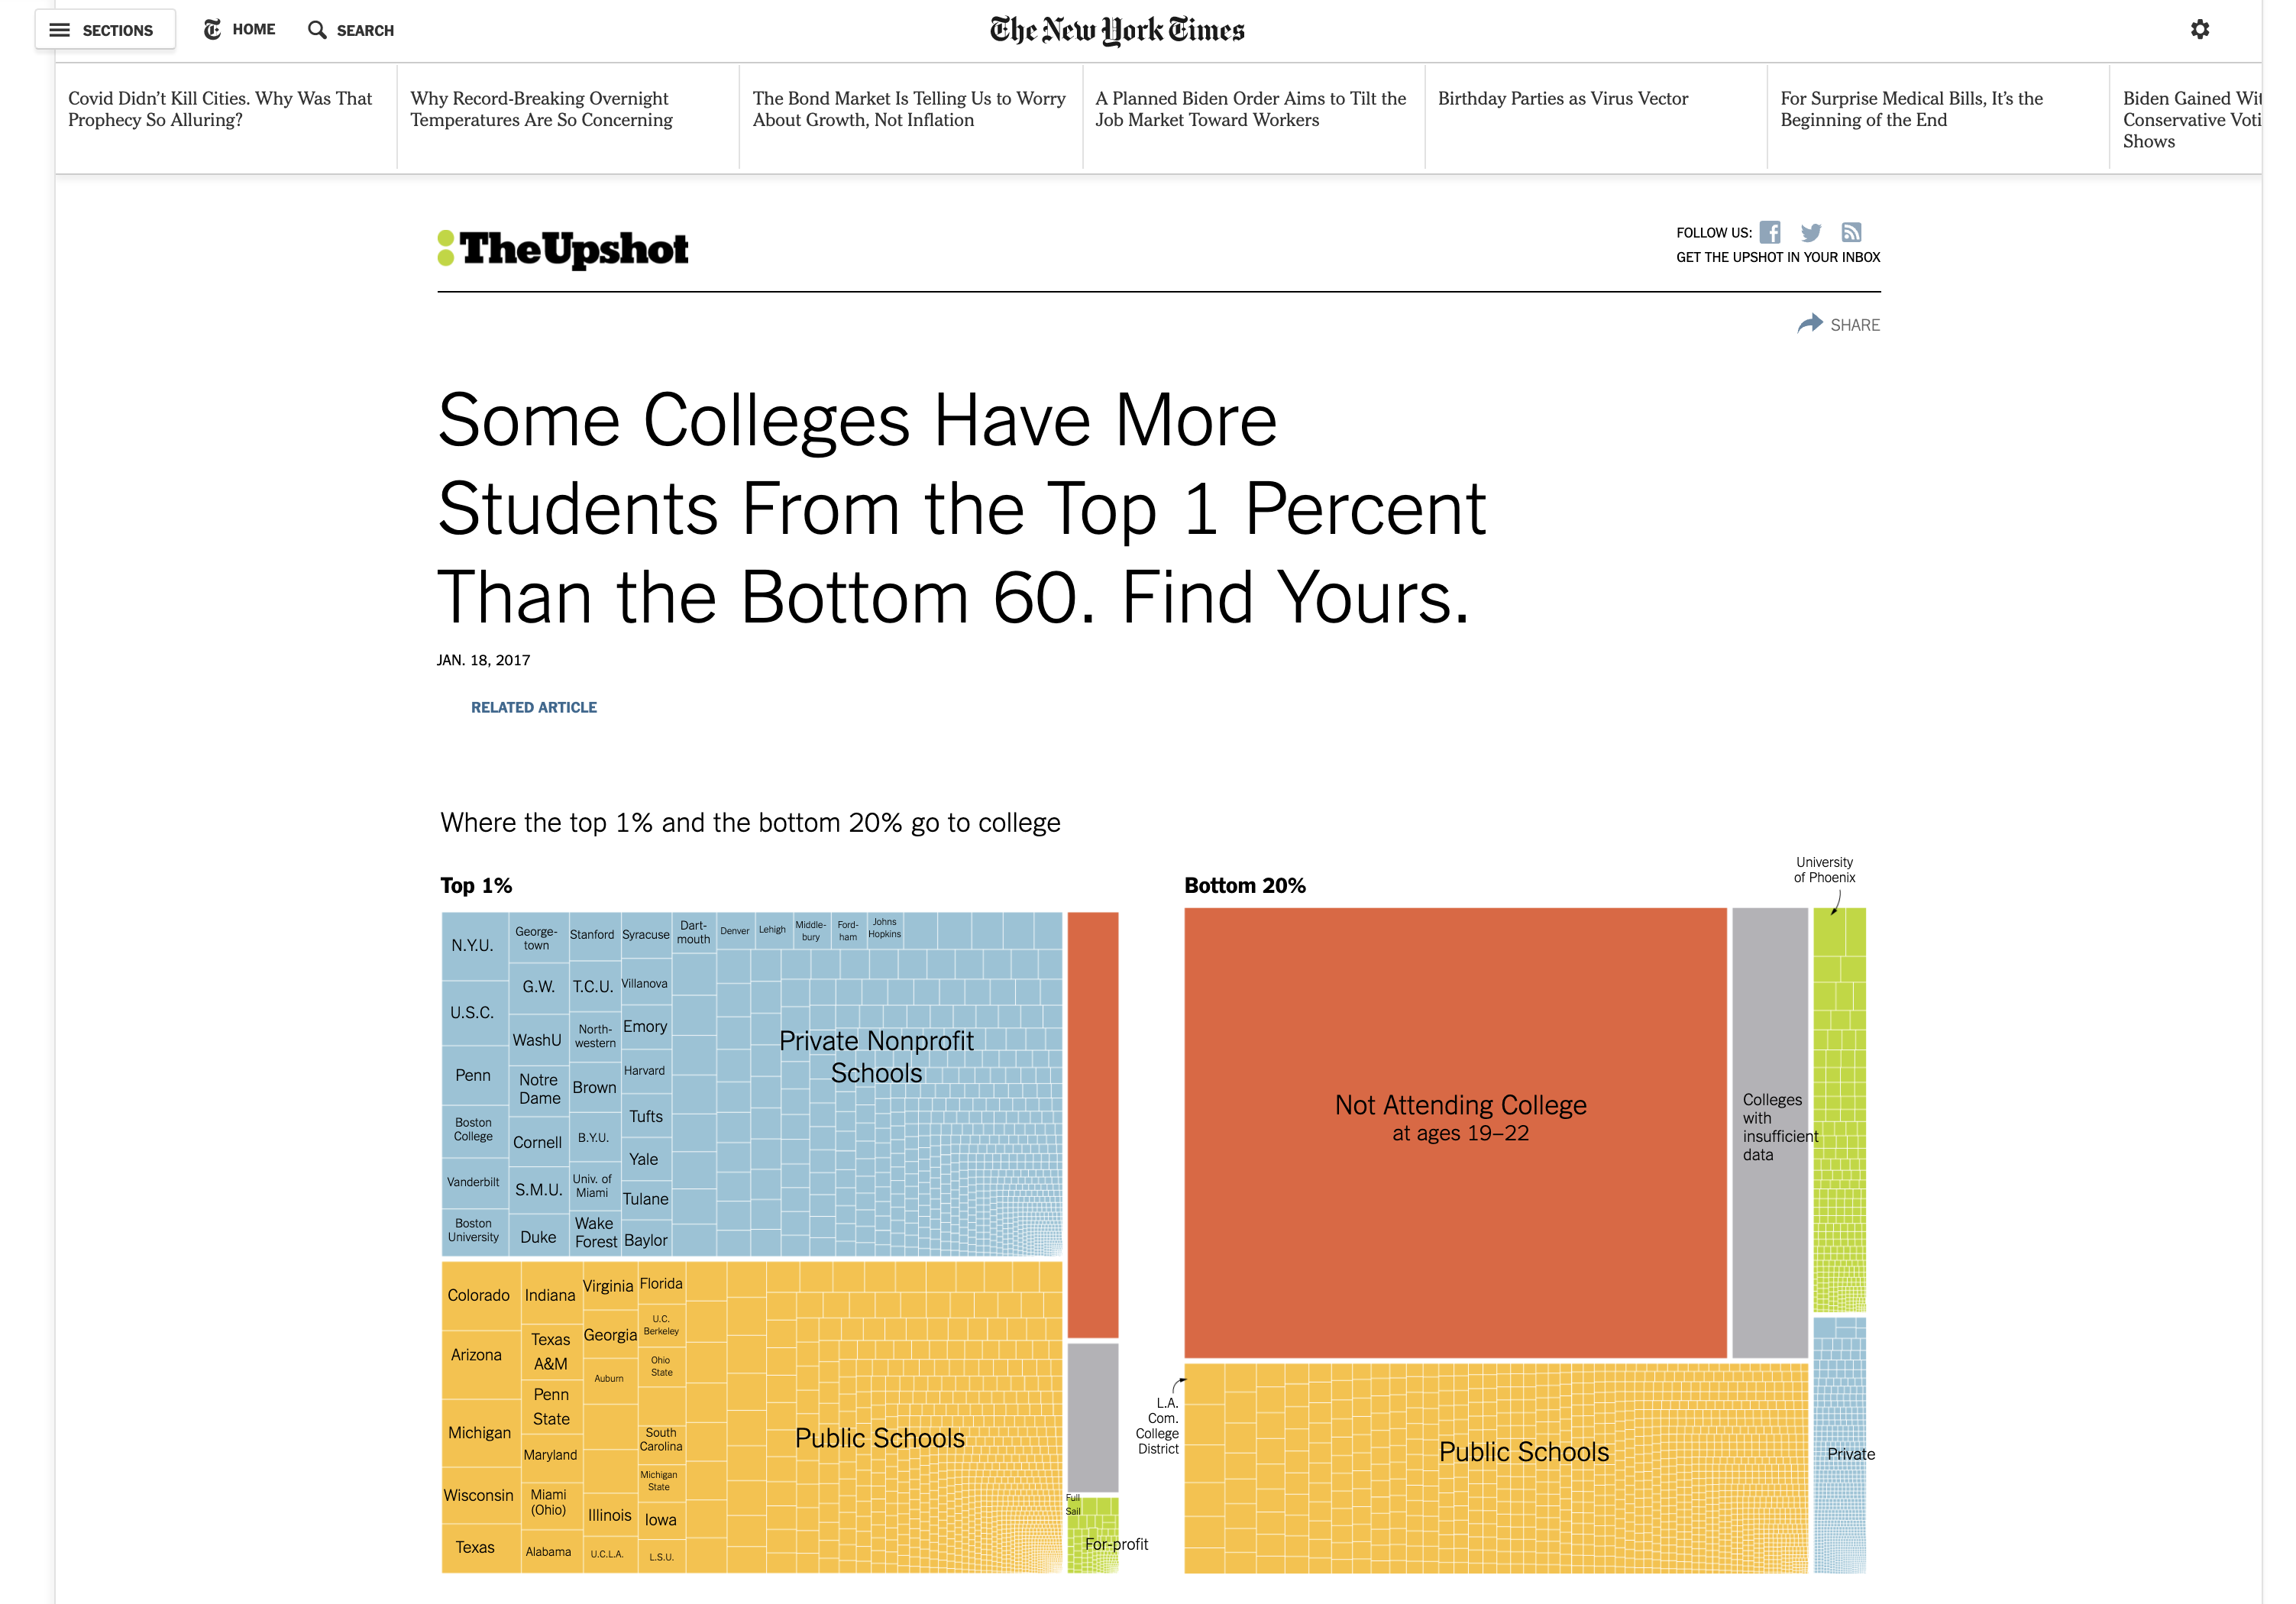
\includegraphics[width=1\linewidth]{images/02_oi} 

}

\caption{New York Times Graphic on Opportunity Insights}\label{fig:oi}
\end{figure}

Let's get a little bit more into the details on what data we will be using in this empirical application. The data comes from federal income tax returns. Researchers at Opportunity Insights have linked to federal tax returns to tax records of universities and data from Pell grants. The result is a dataset with (1) Children linked to their parents (children are reported as dependents) (2) Income data for both children and parents and (3) children linked to the universities they attended.

This will give us everything we need to know to understand how a given college promotes intergenerational mobility. It will allow us to know both the know both the background of students attending a given college as well as their eventual earnings. It is important to emphasize that this was a huge data task that gives us a new way to study an important question. This comprehensive data has only recently become available.

We have discussed at a high level the concept of intergenerational mobility. But when we turn to the data, we will need to compute a metric of intergenerational mobility that allows us to compare across colleges. Before introducing this measure, we will introduce a statistical concept that will be important throughout the course, and in particular, in understanding our measure of intergenerational mobility: \textbf{quantiles}.

  \bibliography{book.bib,packages.bib}

\end{document}
